\documentclass[frenchle,a4paper,12pt,twoside]{refrep}
\title{Manuel de l'utilisateur}


% Set the page title
\newcommand{\mycontent}[0]{
\begin{tabular}{l}
\hspace*{-4cm} \em XCSoar: Manuel de l'utilisateur \vspace*{2pt}
\end{tabular}}

\usepackage{color}
\usepackage{times}
\usepackage{booktabs}
\usepackage{longtable}
\usepackage{rotating}
\usepackage{todonotes}
\usepackage{multirow}
\usepackage{makeidx}\makeindex
\makeatletter
\usepackage{fancyhdr}
\pagestyle{fancy}
\maxipagerulefalse
%
% Include XCSoar header and footer settings and used buttons
\input{xcsoar-headers.sty}
\definecolor{buttongray}{rgb}{0.831,0.816,0.784}
\newcommand{\blink}[0]{$\triangleright$}
\newcommand{\bmenu}[1]{
	\fcolorbox {black}{buttongray}{{\sf{#1}}}
}
\newcommand{\bmenut}[2]{
	\fcolorbox {black}{buttongray}{
    \makebox[1.4cm][c]{
    	\begin{tabular}{c}
    	{\footnotesize\sf{#1}}\\
    	{\footnotesize\sf{#2}}
    	\end{tabular}
    }
  }
}
\newcommand{\bmenuth}[3]{
	\fcolorbox {black}{buttongray}{
    \makebox[1.4cm][c]{
    	\begin{tabular}{c}
    	{\footnotesize\sf{#1}}\\
    	{\footnotesize\sf{#2}}\\
    	{\footnotesize\sf{#3}}
    	\end{tabular}
    }
  }
}
\newcommand{\bmenus}[1]{
	\fcolorbox {black}{buttongray}{
    \makebox[1.4cm][c]{
      \begin{tabular}{c}
        {\footnotesize\sf{#1}}\\
    	  \\
      \end{tabular}
	  }
	}
}
\newcommand{\button}[1]{
	\fcolorbox {black}{buttongray}{{\sf #1}}
}

\newcommand{\infobox}[1]{
	\fcolorbox {black}{white}{\makebox[1.7cm][c]{\sf #1}}
}


\newenvironment{jspecs}{
\itemsep=2pt\topsep=3pt\partopsep=3pt\parskip=0pt
\begin{description}
\itemsep=2pt\topsep=3pt\partopsep=3pt\parskip=0pt
}
{\end{description}}

\newcommand{\jindent}[2]{
  \noindent\makebox[0pt][r]{{#1}\hspace*{\marginparsep}}
  \parbox[t]{0.95\linewidth}{#2}\par
}

%
\widowpenalty=1000
\clubpenalty=1000
%
%  XCSoar - Website Einfügen
\newcommand{\xcsoarwebsite}[0]{\url{www.xcsoar.org}}
%
% Define command to insert tip image
\newcommand{\tip}[0]{\marginlabel{\parbox{1.1cm}{
\includegraphics[width=0.7cm]{figures/reminder.pdf}}}}

% Define command to insert gesture image
%\newcommand{\gesture}[1]{\marginlabel{{\it#1{\phantom{aa}}}\parbox{1.1cm}{\hspace{-3mm}
\includegraphics[width=0.8cm]{figures/gesture.png}}}}
\newcommand{\gesture}[1]{\marginlabel{{\it#1{\phantom{aa}}}\parbox{1.1cm}{\hspace{-3mm}
\includegraphics[width=0.8cm]{figures/gesture.pdf}}}}
%
% Define command to insert warning image
\newcommand{\warning}[0]{\marginlabel{\parbox{1.3cm}{
\includegraphics[width=0.9cm]{figures/warning.pdf}}}}
%
% Define command to insert Achtung image
\newcommand{\achtung}[0]{\marginlabel{\parbox{1.3cm}{
\includegraphics[width=2.5em]{figures/warning.pdf}}}}
%
% Define command to insert a flash image
\newcommand{\blitz}[0]{\marginlabel{\parbox{1.3cm}{
\includegraphics[height=2.0em]{figures/reminder.pdf}}}}
%
% Define command to insert a stop
\newcommand{\halt}[0]{\marginlabel{\parbox{1.3cm}{
\includegraphics[height=2.0em]{figures/warning.pdf}}}}
%
% Define command to reference a configuration item
\newcommand{\config}[1]{\marginlabel{\ref{conf:#1}\parbox{1.3cm}{
\includegraphics[width=0.8cm]{figures/config.pdf}}}}
%
% Potentially overdue ``InfoBox'' style macro
\newcommand{\InfoBox}[0]{{InfoBox}}
%
% Define command to put a menu label on the margin
\newcommand{\menulabel}[1]{\marginpar{\parbox{5.0cm}{\raggedright #1}}}
%
% Define command to draw a sketch on the margin
\newcommand{\sketch}[1]{\marginpar{\parbox{3.750cm}{\includegraphics[angle=0,width=0.9\linewidth,keepaspectratio='true']{#1}}}}
%
% Define command to draw a small sketch on the margin
\newcommand{\smallsketch}[1]{\marginpar{\includegraphics[angle=0,keepaspectratio='true']{#1}}}
%
% Enumerated todo's for the todonotes package
\newcounter{todocounter}
\newcommand{\todonum}[2][]{\stepcounter{todocounter}\todo[#1]{\thetodocounter: #2}}
%
% dies nette Makro bringt mir die aktuelle Version der bearbeiteten XCSoar-Verrion aufs Papier
\newcommand{\version}{\begingroup\catcode`\_=\active\input{VERSION.txt}\endgroup}
%
%Anführungszeichen per Tastatur einfach so eingeben -> "
%\shorthandoff{"}%

\def\maketitle{%
  \null
  \thispagestyle{empty}%
  \begin{maxipage}
    \begin{center}
    
\includegraphics[angle=0,width=0.5\textwidth,keepaspectratio='true']{graphics/logo.pdf}
    \vskip 0.5cm
    
\includegraphics[angle=0,width=0.66\textwidth,keepaspectratio='true']{graphics/title.pdf}
    \end{center}
    \begin{center}
      \normalfont\huge\textsf{La Navigation Open Source}\par
    \end{center}
    \vskip 1cm
    \begin{center}
      \normalfont\huge\textsf{\@title}\par
    \end{center}
    \vskip 1cm
  \end{maxipage}

  \vfill
  \todo[nolist,size=\Large,inline]{Traduction en cours, v�rifiez qu'il n'y a pas de version plus r�cente avant d'imprimer.}

  \begin{flushright}
    \large \strut {
      \sf
      \today \\
      XCSoar version \version \\
      \xcsoarwebsite{} \\
    } 
    \par
  \end{flushright}
  \par
  \vfil
  \vfil
  \null
  \cleardoublepage
}

\usepackage[utf8]{inputenc}
\DeclareUnicodeCharacter{00B0}{$^{\circ}$}
\usepackage{xkeyval}
\usepackage[frenchle]{babel}
\begin{document}
\maketitle

%%%%%%%%%%%%%%%%%%%%%%
\listoftodos

%cela est toujours le cas quand le Goto automatique existe ???
%\tip It is also possible to save a `default' task and have this task loaded
%automatically upon start-up of XCSoar.  One application of this is to
%set up a default task with one waypoint being the home --- this means
%that XCSoar is then programmed for final glide back to home, which is
%useful for casual cross-country touring.


\warning
CE MANUEL EST EN COURS DE TRADUCTION!
IL N'EST PAS VRAIMENT UTILE ET TRÈS ÉCOLOGIQUE DE L'IMPRIMER VU QU'IL VA ENCORE BEAUCOUP ÉVOLUER ET QU'IL RESTE PAS MAL DE TEXTE EN ANGLAIS.
IL PEUT AUSSI CONTENIR DES ERREURS!!!
POUR SIGNALER CE GENRE DE CHOSES... VOUS POUVEZ CONTACTER Daniel: osteocool@yahoo.fr

MERCI
%%%%%%%%%%%%%%%%%%%%%%
\begingroup
\setlength{\parskip}{0.1\baselineskip}
\tableofcontents
\endgroup

%%%%%%%%%%%%%%%%%%%%%%
\chapter*{Préface}

\section*{Avertissements et précautions d'utilisation}

\warning IL EST DE LA RESPONSABILITÉ DE L'UTILISATEUR D'UTILISER CE LOGICIEL AVEC LA PLUS GRANDE PRUDENCE. CE LOGICIEL EST DESTINE A ETRE UTILISE UNIQUEMENT COMME UNE AIDE A LA NAVIGATION ET NE DOIT PAS ÊTRE UTILISÉ DANS LES CAS EXIGEANT UNE MESURE PRECISE DU CAP,DE LA DISTANCE, DE LA POSITION OU DE LA TOPOGRAPHIE. CE LOGICIEL NE DOIT PAS ÊTRE UTILISÉ COMME AIDE POUR DÉTERMINER L’ALTITUDE EN NAVIGATION AERIENNE. CE LOGICIEL NE DOIT PAS ÊTRE UTILISÉ COMME UN SYSTEME ANTI\-COLLISION.

\section*{Mentions légales}

\subsection*{Contrat de licence logicielle}

Ce logiciel est distribué conformément à la licence GNU « General Public License » Version~3. Voir l'annexe (~\ref{cha:gnu-general-public}) pour le texte complet de l’accord de licence et des provisions de garantie.

\subsection*{Limitation de responsabilité}

En aucun cas, XCSoar, ses dirigeants, actionnaires, cadres, employés, sociétés affiliées, sous-traitants, filiales, ne peuvent être tenues responsables des dommages accessoires, indirects ou dommages-intérêts punitifs de toute nature, suite à l'utilisation du produit.

\subsection*{Avertissement}

Ce produit, et tous les fichiers joints, données ou documents, sont distribués «tels quels» et sans garantie d'aucune sorte, expresse ou implicite. Ce produit est utilisé entièrement sous la responsabilité de l'utilisateur. Bien qu'un grand soin ait été pris pour identifier les éventuelles erreurs pendant
le développement, il n’est en aucun cas revendiqué comme exempt de tout défaut . Aucune garantie n’est fournie quant à son exactitude, sa fiabilité ou son adéquation à un besoin particulier. Les développeurs  et les contributeurs du projet XCSoar ne peuvent en aucun cas être tenu responsables des erreurs pouvant s’y trouver ou des dommages fortuits ou consécutifs, de toute perte de données ou de tout dommages corporels pouvant survenir dans le cadre de la livraison, de la mise en service ou de l'utilisation de ce programme.


%%%%%%%%%%%%%%%%%%%%%%
\chapter{Introduction}\label{cha:introduction}
Ce document est le manuel d'utilistion de XCSoar, logiciel de navigation aérienne, open-source développé à l'origine pour les Poket PC. Le lecteur est sensé avoir de bonnes connaissances des fondamentaux de la théorie  du vol à voile et un minimum de pratique du vol sur la campagne.

Les mises à jour périodiques du logiciel peuvent rendre ce manuel périmé concernant certains points. Il est souhaitable de lire les notes de mise à jour du logiciel pour en connaitre les évolutions. Les mises à jour du logiciel et de la documentation sont disponibles sur
\begin{quote}
\xcsoarwebsite{/download}
\end{quote}

\section{Organisation du manuel}

\todonum[inline]{Write about the manual crossref hinting icons and the yellow
colour. The Quickstart will be readable also without those links available}
Ce manuel est structuré par grandes fonctionnalités du point de vue du pilote. La suite de ce chapitre parle du téléchargement, de l'installation et du lancement du logiciel sur les différentes plateformes matérielles supportées. Le chapitre ~\ref{cha:interface} décrit les concepts de l'interface utilisateur et donne une vue générale de l'affichage.

Le chapitre~\ref{cha:navigation} décrit en détail l'utilisation de la carte mobile et l'aide que peut apporter le logiciel de navigation. Le chapitre~\ref{cha:tasks} décrit comment les circuits sont définis et utilisés en vol. Il présente aussi les outils d'analyse permettant aux pilotes d'améliorer leurs performances. Le chapitre~\ref{cha:glide}  est consacré au calculateur de vol d'XCSoar et présente en détail les fonctionnalités qu'il offre. Il est important pour les pilotes de comprendre comment le calculateur effectue ses différents calculs.

Le chapitre~\ref{cha:atmosph} parle de l'interfaçage du calculateur avec des varios et autres instruments de mesure et comment ces données sont utilisées pour représenter différents modèles concernant entre autre le vent et la convection. Le chapitre~\ref{cha:airspace} parle de la gestion des espaces aériens et des alarmes dédiées ainsi que des alarmes du FLARM. Le chapitre~\ref{cha:avionics-airframe} présente l'intégration du calculateur avec le reste des systèmes utilisés dans l'environnement de vol ( terminaux permettant de communiquer avec le calculateur, switches divers) et des diagnostiques possibles.

La suite du document est constituée principalement de chapitres de référence. Le chapitre~\ref{cha:infobox} liste les différentes informations qui peuvent être affichées dans les "InfoBox" sur les côtés de la carte mobile. La configuration du logiciel est décrite dans le chapitre ~\ref{cha:configuration}. Le format des fichiers utilisés ainsi que la manière de les obtenir ou les créer et les éditer est décrit dans le chapitre~\ref{cha:data-files}.

Enfin, un bref historique et une explication du processus de développement de XCSoar sont présentés dans le chapitre ~\ref{cha:history-development}.

\section{Remarques}

\subsection*{Terminologie}
Un certain nombre de termes sont utilisés pour la description de matériel embarqués tels que Pocket PC, comprenant 'organiser', Portable Digital Assistant (PDA), et Personal Navigation Assistant (PNA). XCSoar est aussi disponible sur plateforme Altair(calculateur Triadis) qui est concrètement un instrument de navigation et plusieurs autres plateformes. Dans ce document ces termes sont utilisés indifféremment comme référence à un matériel supporté par XCSoar.

\subsection*{Copies d'écran}
Tout au long de ce manuel des copies d'écran de XCSoar sont présentées. Elles proviennent de différentes plateformes matériel et pas forcément de la même version d'XCSoar. Entre plateforme il peut y avoir des différences de résolution d'écran, de présentation générale, de police de caractères ce qui induit des différences entre la documentation et la visualisation sur l'appareil. La plupart des copies d'écran de ce manuel sont faites avec un affichage d'XCSoar en format paysage.

\section{Platformes}
\begin{description}
\item[Windows PC]
XCSoar fonctionne sur un PC sous Windows (XP, Vista, 7 versions 32 et 64 bits). Cette version est principalement utile pour la prise en main, l'entrainement à l'utilisation d'XCSoar, rejouer des fichiers IGC enregistrés ou utiliser XCSoar en mode simulation sur un PC non connecté à un GPS.
\item[Windows Mobile PDA/PNA]
XCSoar supporte les appareils utilisant Microsoft Pocket PC 2000 jusqu'à Windows Mobile 6. Windows Mobile 7 n'est pas supporté car Microsoft a décidé de ne pas maintenir les applications natives à partir de cette version.
\item[Unix/Linux PC]
XCSoar peut tourner sous Unix en utilisant l'émulateur Wine. Une version native Unix existe à partir de la version 6.0 mais est toujours considérée comme expérimentale.
\item[Périphériques Androïd] supporté à partir d'Androïd 1.6 et versions ultérieures.
\item[Altair] Le calculateur de vol Altair, de triadis engineering GmbH, dans lequel XCSoar est pré-installé. la version Altair PRO comporte un GS interne.
\end{description}



\section{Support technique}

\subsection*{Dépannage}
XCSoar est développé par une petite équipe. Bien que nous soyons heureux de vous aider dans l'utilisation de notre logiciel, nous ne pouvons donner de cours sur l'utilisation des techniques modernes d'information!
Si vous avez des questions concernant XCSoar, consultez la FAQ en premier lieu. Si vous ne trouvez pas de réponse satisfaisante, envoyez un mail à la liste:
\begin{quote}
\href{mailto:xcsoar-user@lists.sourceforge.net}{xcsoar-user@lists.sourceforge.net}
\end{quote}

Les nouvelles questions seront ajoutées à la FAQ du site de XCSoar.

Vous pouvez aussi vous inscrire à la liste de mails de XCSoar afin d'être averti des derniers développements du logiciel. Pour plus d'information voir sur notre site:
\begin{quote}
\xcsoarwebsite{/discover/mailinglist.html}
\end{quote}

Le fichier de "log" du démarrage du logiciel est \verb|xcsoar-startup.log|. Il peut être envoyé aux développeurs d'XCSoar pour les aider à déterminer les causes de problèmes au lancement du logiciel.

Pour les utilisateurs d'Altair le fichier de log est transféré vers le répertoire `FromAltair' à l'aide d'AltairSync si un support de stockage USB est connecté et qu'Altair est déjà sous tension.

\subsection*{Mises à jour}
Il est souhaitable de visiter le site web de XCSoar pour vérifier si il n'y a pas de mise à jour disponible. La procédure d'installation décrite au chapitre~\ref{cha:installation} suivant peut être répétée pour la mise à jour du logiciel. Les fichiers de configurations et les données personnelles (cartes, points de virage,...) sont préservées lors des mises à jour et ré-installations.

Il est bien entendu recommandé de mettre à jour les données de navigation (cartes, espaces aériens) pouvant être modifiées par les autorités. Le fichier d'espace aérien mis à disposition sur le site de la FFVV est mis à jour environ une fois par mois au cours de la saison.

\subsection*{Mises à jour de XCSoar sur Altair}
La lise à jour du logiciel sur Altair implique de télécharger le dernier fichier {\tt XCSoarAltair-YYY-CRCXX.exe} et de le copier sur une clé USB ou une carte SD. Ensuite utiliser l'utilitaire AltairSync sur le terminal Altair pour terminer l'installation. Pour plus de détails, se référer au {\em Manuel d'utilisateur Altair}.

Les autres types de données ou programmes peuvent être installés sur Altair de la même façon.

\subsection*{Vos retours}
Comme tout programme élaboré, XCSoar peut comporter des bugs. Si vous en trouvez un, veuillez le remonter à l'équipe de développement en utilisant notre portail dédié à:
\begin{quote}
\xcsoarwebsite{/trac}
\end{quote}
ou en nous contactant par mail à:

\begin{quote}
\href{mailto:xcsoar-devel@lists.sourceforge.net}{xcsoar-devel@lists.sourceforge.net}
\end{quote}

\section{Entrainement}
Pour votre sécurité et celle des autres, les pilotes utilisant XCSoar doivent s'entrainer à l'utilisation du logiciel, au sol , afin de s'habituer à l'interface utilisateur et au différentes fonctionnalités qu'il offre, AVANT de l'utiliser en vol.

\subsection*{XCSoar sur un PC}
La version PC permet de se familiariser avec le logiciel, son interface utilisateur et ses fonctionnalités tout en étant confortablement installé à la maison, une bière à la main.... Tous les fichiers et les configurations de cette version sont identiques aux versions embarquées. Il est donc très facile de tester différentes configurations sur le PC avant de les mettre en pratique en vol.

La version PC peut être connectée à des instruments et fonctionner comme un calculateur en l'air. Exemples d'utilisation:

\begin{itemize}
\item Connecter un FLARM au PC pour utiliser XCSoar comme station au sol, pour afficher le traffic des planeurs équipées de FLARM.
\item Connecter un variomètre "intelligent"  comme le Vega pour tester le paramétrage du vario.
\end{itemize}

\subsection*{XCSoar avec un simulateur de vol}
Une bonne manière d'apprendre à se servir du logiciel est de connecter un Pocket PC à un PC sur lequel tourne un simulateur de vol qui peut envoyer des messages NMEA vers un port série. Condor et X-Plane le permettent par exemple.

Le gros avantage de s'entrainer ainsi est que XCSoar peut être utilisé en mode FLY. Ainsi, il se comporte exactement comme si vous voliez et vous pouvez avoir un très bon aperçu du fonctionnement de XCSoar quand vous utilisez le simulateur de vol.

\section{XCSoar et la sécurité}
L'utilisation d'un calculateur tel que XCSoar en vol entraine certains risques: l'attention du pilote peut être diminuée de manière très significative, comme le temps passé à regarder en dehors du cockpit pour assurer la sécurité.

La philosophie guidant la conception et le développement de XCSoar est de réduire cette distraction en minimisant les interactions de l'utilisateur et en présentant les informations de façon claire et lisible d'un coup d'œil.

Les pilotes qui utilisent ce logiciel sont responsables de l'utilisation de XCSoar en sécurité.
Pour bien utiliser XCSoar vous devez:
\begin{itemize}
\item Devenir familier avec l'interface graphique et avec vous entrainer au sol.
\item En vol, prendre l'habitude de regarder dehors autour de vous avant d'interagir avec le logiciel.
\item Configurer le logiciel pour profiter des fonctionnalités automatisées pour minimiser les interactions avec le logiciel. Si vous vous apercevez que vous faites mécaniquement des actions fréquentes, demandez-vous (ou à un autre utilisateur de XCSoar) si le logiciel ne peut pas être configuré pour le faire à votre place.
\end{itemize}

\chapter{Installation}\label{cha:installation}

Um {\textsf  XCSoar} zum Laufen zu bringen benötigst Du folgendes:


\begin{itemize}
\item ein Gerät, auf dem {\textsf  XCSoar} läuft.
\item {\textsf  XCSoar} an sich
\item einen GPS Empfänger
\item ein Wegpunkt-File
\item ein Luftraum-File
\item ein Karten-File (Kartendatenbank bzw. Gelände)
\end{itemize}

\section{Kompatibilität}

\subsection*{Geräte auf denen  {\textsf  XCSoar} läuft}

{\textsf  XCSoar} läuft derzeit auf folgenden Plattformen:

\begin{itemize}
\item Handys und Tablets mit Android 1.6 oder neuer\\
  Beispiel: Dell Streak, Samsung Galaxy S II, HTC Desire HD, Samsung Tablet 10.1N
  Motorola Xoom
\item PDAs mit Pocket PC 2000, 2002, 2003 \\
  Beispiel: Asus A600, Compaq iPaq 3800, 38xx, iPaq 3900, 39xx
\item PDAs mit Windows Mobile \\
  Beispiel: iPaq hx4700, Dell Axim x51v
\item PNAs mit  Windows CE 3.0 oder neuer \\
  Beispiel: HP314, Mio400
\item Triadis Altair
\item LX MiniMap
\item Windows 2000 oder neuer
\item Linux
\item Mac OS X
\end{itemize}

\subsection*{GPS, Logger, Varios}

{\textsf  XCSoar}  ist kompatibel zu allen Geräten, welche GPS-Daten im NMEA-Format ausgeben.

Die meisten modernen Android Geräte haben einen eingebauten GPS-Empfänger, der diese Daten zur Verwendung 
ausgibt. Mitunter jedoch ist es ratsam, diese Daten aus einem anderen Gerät zu verwenden, wenn man z..B.\ Luftverkehrsdaten aus einem 
\fl benutzen und anzeigen möchte oder aber noch weitere Features -wie nachfolgend aufgelistet- nutzen möchte:



\begin{itemize}
\item Geschwindigkeitssensor (TAS) erlaubt schnelle und eine exakte Ermittlung des Winds ohne Kurbeln zu müssen
\item ein extern angeschlossenes Vario wird die Zentrierhilfe unterstützen und erheblich beschleunigen
\item Aufgaben können deklariert und ausgetauscht werden (laden und speichern z.B. in IGC Logger ),   Flüge können ausgelesen werden 
\item manche Varios erlauben eine Synchronisation z.B.\ des MC-Wertes und anderen Werte mit {\textsf  XCSoar} 
\end{itemize}

\subsection*{Unterstützte externe Geräte und deren Funktionen}\label{sec:supported-varios}

\newcommand{\y}[0]{{ $\surd$ }}
%{0.8\textwidth}
\noindent\makebox[\textwidth]{%
\begin{tabular}{l|ccc|cc|cc|c}
       \multicolumn{1}{r}{\bf Unterstütze:} & \multicolumn{3}{c|}{\bf -Funktionen} & \multicolumn{5}{c}{\bf -Daten} \\
NMEA Gerät & 
  \begin{sideways} Deklaration\end{sideways} & 
  \begin{sideways} Fernbedienung\end{sideways} & 
  \begin{sideways} Download\end{sideways} &
  \begin{sideways} TAS \end{sideways} & 
  \begin{sideways} Vario\end{sideways} & 
  \begin{sideways} Baro. Höhe\end{sideways} & 
  \begin{sideways} Wind\end{sideways} &
  \begin{sideways} G-Sensor\end{sideways} \\
\hline
%                    _Decl_Remo_Down_Airs_Vari_Baro_Wind_Gsen_
Borgelt B50          &    & \y &    & \y & \y & \y &    &    \\
CAI 302              & \y & \y & \y & \y & \y & \y & \y & \y \\
CAI GPS Nav          &    &    &    &    &    &    &    &    \\
Condor               &    &    &    & \y & \y & \y & \y &    \\
\hline
Digifly Leonardo     &    &    &    & \y & \y & \y & \y &    \\
EW Logger            & \y &    &    &    &    & \y &    &    \\
EW microRecorder     & \y &    &    &    &    & \y &    &    \\
FLARM                & \y &   & \y  &    &    & \y &    &    \\
\hline
%                    _Decl_Remo_Down_Airs_Vari_Baro_Wind_Gsen_
Flymaster F1         &    &    &    &    & \y & \y &    &    \\
Flytec 5030          &    &    &    & \y & \y &    &    &    \\
GTAltimeter          &    &    &    &    &(\y)& \y &    &    \\
ILEC SN10            &    &    &    &    & \y & \y & \y &    \\
\hline
IMI ERIXX            & \y &    & \y &    &    &    &    &    \\
LX20, Colibri        & \y &    & \y &    &    & \y &    &    \\
LX Vario \footnotemark
                     & \y & \y &    & \y & \y & \y & \y & \y \\

LXNAV Nano           & \y &    &    &    &    &    &    &    \\
\hline
%                    _Decl_Remo_Down_Airs_Vari_Baro_Wind_Gsen_
LXNAV V7             &    & \y &    & \y & \y &    &    &    \\
PosiGraph            & \y &    &    &    &    & \y &    &    \\
Triadis Altair (pro) & \y &    &    &    &    & \y &    &    \\
Triadis Vega         &    & \y &    & \y & \y & \y &    & \y \\
\hline
Volkslogger          & \y &    &    &    &    & \y &    &    \\
Westerboer VW1150    &    & \y &    & \y & \y & \y &    &    \\
Westerboer VW921, 922
                     &    & \y &    & \y & \y & \y &    &    \\
Zander / SDI         &    & \y &    & \y & \y & \y & \y &    \\

\end{tabular}}
\footnotetext{LX Navigation biete mehrere ''intelligente'' Varios an, wie z.B.\ 
  LX1600, LX5000, LX7000. All diese bieten den gleichen NMEA-Ausgang
  Die angebotenen Funktionen in Verbindung mit {\textsf  XCSoar} hängen jedoch zum Großteil auch von der 
Firmware des benutzten  Gerätes ab.}



Während die meisten CE-basierten Geräte über eine serielle Schnittstelle verfügen, 
ist diese Art der Schnittstelle bei den meisten, modernen Android-Geräten nicht mehr vorhanden. 
Diese können entweder Bluetooth oder aber das Android IOIO-Board verwenden. 


Um Bluetooth zu benutzen, verbinde das Gerät mit einem Bluetooth $\leftrightarrow$ Seriell-Adapter, wie z.B.\ 
 dem K6-Bt oder dem Glidertools VFBT-1.


\section{Software Installation der Software}\index{Installation}

Die Software ist auf der {\textsf  XCSoar}-Homepage frei herunterzuladen. 
In diesem Kapitel wird behandelt, {\sl wie} die Software heruntergeladen und installiert wird.

\subsection*{Betriebssystem Android}\index{Installation!unter Android}

Suche nach {\textsf  XCSoar} in Googles Android-Marktplatz (PlayGround), oder installiere das \verb|apk|-
File manuell.  Kopiere diese Datei auf eine SD-Karte in das Verzeichnis \verb|XCSoarData|.

\subsection*{Auf einem PDA (Windows Mobile, PocketPC)}\index{Installation!unter Pocket PC, Windows Mobile}

Wähle eines dieser Files:

\begin{description}
\item[\texttt{PPC2000}] Pocket PC 2000/2002, Windows CE 3.0
\item[\texttt{PPC2003}] Pocket PC 2003, Windows CE 4.0
\item[\texttt{WM5}] Windows Mobile 5 oder neuer
\item[\texttt{WM5X}]Windows Mobile 5 oder neuer mit XScale CPU oder besser(z.B. hx4700)
\end{description}

\sketch{figures/XCS_Today.png}
Lade das File \verb|XCSoar.exe| herunter und kopiere es auf eine SD Karte.  
Starte das File z.B.\ über den Explorer. 

Ein andere Methode ist, {\textsf  XCSoar} auf PDA über das CAB-File zu installieren.  Lade dies File herunter auf Deine SD-Karte, 
anschließend  doppelklicke darauf und {\textsf  XCSoar} wird auf Deinem PDA installiert werden. 

Nach der Installation werden das {\textsf  XCSoar}-Symbol sowie die beiden Schriftzüge ''FLY'' und ''SIM'' aufgelistet
dem ''Heute''-Schirm sichtbar sein. (s.\ Bild) 


\subsection*{Auf einem PNA (Windows CE)}\index{Installation!unter Windows CE}

Lade das File \verb|XCSoar.exe| (Ziel wie oben ''WM5'') auf eine SD Karte herunter. 
Führe es z.B.\ mit dem Explorer aus.

\subsection*{Auf einem Windows PC}\index{Installation!unter Windows}
  
Lade das entsprechende File \verb|XCSoar.exe| (Ziel ''PC'') auf Deinen Rechner (Platte) herunter und führe es aus.


\subsection*{Unter Unix/Linux}\index{Installation!unter Linux}

Das herunterzuladende File ist \verb|xcsoar_XXX.deb|, wobei \verb|XXX| die Version und Plattform darstellt.  
z.B.\ \verb|xcsoar_6.0.4_i386.deb|. Dies ist ein Debian Paket und für 32bit Betriebssysteme mit Intel-Prozessoren gedacht.
Es kann installiert werden mit:
\begin{center}
\verb|sudo dpkg -i xcsoar_XXX.deb|.
\end{center}
Um zu sehen, wo die ausführbaren Dateien und die anderen Dateien installiert wurden, führe \verb|dpkg-query -L xcsoar| 
aus. 

Alle weiteren Dateien (Karten, Lufträume etc.\ müssen in \verb|~/.xcsoar/XCSoarData/| kopiert werden.
Wenn das Verzeichnis \verb|~/.xcsoar| nicht existiert, wird es beim ersten Aufruf von {\textsf  XCSoar} angelegt.


\section{Daten Files}\label{InstallationDatenfiles}\index{Installation!Datenfiles}

Um alle Funktionen von {\textsf  XCSoar} nutzen zu können, werden weitere Daten und Files benötigt.
Hierzu zählen Lufträume, Geländedaten, Topologiedaten eine Polare, Wegpunkte und so weiter. 


Die Nutzung dieser Daten und Files wird in Kap.~\ref{cha:data-files} ausführlich beschrieben. 

Alle Files sollten unbedingt in das Verzeichnis \texttt{XCSoarData} kopiert bzw. \ gespeichert werden. 
Dies Verzeichnis muß  in einem bekannten Verzeichnis befindlich sein, damit {\textsf  XCSoar} bekannt ist, wo es nach entsprechenden 
Daten-File suchen muß: 

 
\begin{description}
\item[Windows PC]
\texttt{XCSoarData} befindet sich im Persönlichen Verzeichnis (''\texttt{Eigene Dateien}'')
\item[Windows Mobile PDA/PNA]
- Wenn ein Verzeichnis \texttt{XCSoarData} im gleichen Verzeichnis wie {\textsf  XCSoar} existiert, dann wird dies benutzt.  


- \texttt{XCSoarData} befindet sich auf der SD-Karte.  Wenn keine SD-Karte vorhanden ist, dann schaut {\textsf  XCSoar} in \texttt{Eigene Dateien} nach diesen Files

\item[Unix/Linux]
Das Verzeichnis heißt \verb|.xcsoar| und befindet sich im \verb|home| - Verzeichnis des Users. 
\item[Android Geräte]
\texttt{XCSoarData} befindet sich auf der SD-Karte.
\item[Altair]
Wenn {\textsf  XCSoar} sich auf einem USB-gerät (Stick) befindet, dann wir dies benutzt, andernfalls wird der interne Speicher benutzt. 
\end{description}


{\textsf  XCSoar} wird während der Laufzeit einige zusätzliche Files, wie z.B.\ eine Datei mit sämtlichen Konfigurationsdetails erzeugen.
Diese werden ebenfalls im \texttt{XCSoarData} Verzeichnis (Windows PC und Windows Mobile Geräte), oder aber im \texttt{.xcsoar} 
Verzeichnis(Unix/LinuxPC) abgelegt. 

Beim ersten Start wird {\textsf  XCSoar}  folgende Files erzeugen und anlegen: 
\texttt{Default.tsk} (Standard Aufgabe),  \texttt{xcsoar-registry.prf} (Konfigurationseinstellungen), \texttt{xcsoar-startup.log} 
(Ein Log-Schrieb des Startprozesses von {\textsf  XCSoar}\dots), 



Weiterhin werden drei Verzeichnisse angelegt: \texttt{cache}, \texttt{config} und \texttt{logs}.  

Während des Laufes von {\textsf  XCSoar} können (und werden) weitere Files angelegt wie z.B.\  Aufgaben-Files (\texttt{*.tsk}) 
und Flugaufzeichnungen (evtl.\ (\texttt{*.igc})


\section{Betrieb von {\textsf  XCSoar}}
%\subsection*{Fly and simulator modes}

{\textsf  XCSoar} wird kann in zwei Modi ausgeführt werden:
\begin{description}
\item[FLY] Dies ist der ''echte'' Flugmodus. Alle Ein - und Ausgänge betr.\ Signalaustausch sind aktiv
\item[SIM] Dies ist der Simulator-Modus. Keine Kommunikation mit externen Geräten per serieller Schnittstelle möglich. 
\end{description}

\subsection*{\al - Version}
Wenn der \al angeschaltet wird, fährt {\textsf  XCSoar} automatisch hoch (es ist quasi das das ''Betriebssystem'' des \al) 
Der PWR/ESC Knopf hat mehrer Funktionen:
\begin{description}
\item[Anschalten]  Drücken und halten für mehr als eine Sekunde: Die LED beginnt zu leuchten und {\textsf  XCSoar} wird starten, nachdem der \al gebootet hat.
\item[Ausschalten]  Drücken und Halten für mehr als drei Sekunden: Schaltet den Altair und somit {\textsf  XCSoar} aus.
\item[Escape] Kurzes Drücken des Knopfes wirkt wie die ESC-Taste eines PC: Wird benutzt als Abbruch-Funktion oder aber zum 
              Ausschalten von von Dialogen benutzt.
\end{description}

\achtung Die \al-Version von {\textsf  XCSoar} hat keine Simulator-Funktion

\subsection*{{\textsf  XCSoar}-PC Version}
Ein Doppelklick im entsprechenden Verzeichnis {\textsf  XCSoar} öffnet das Programm. 
{\textsf  XCSoar} kann auch mit Kommandozeilenoptionen oder über ein Batch-File mit Parametern geöffnet werden, 
die hier angegeben werden: 

\begin{description}
\item[-portrait] Anzeige ist 480 Pixels breit, 640 Pixels hoch
\item[-square] Die Anzeige ist 480 Pixel breit, 480 Pixel hoch
\item[-landscape] die Anzeige ist 640 Pixel breit, 480 Pixel hoch. Dies ist die Standardeinstellung.
Wenn Du nichts anderes angibst, wird diese Einstellung auf dem PC automatisch gewählt.
\item[-small] Dies stellt den Bildschirm in halber Größe dar. sinnvoll z.B.\ wenn {\textsf  XCSoar} in Verbindung mit dem Segelflugsimulator 
{\sc Condor} für das Trainig (oder gegen Langeweile) im Winter gestartet wird.
\end{description}

Um die Bildschirmdarstellung zu ändern ist es sinnvoll, sich in Windows eine Verknüpfung herzustellen. 
In den ''Eigenschaften'' sollte dann unter ''Ziel'' der Programm zusammen mit den Kommandozeilenparametern 
angegeben werden. (z.B.\ \texttt{xcsoar.exe -landscape}


\subsection*{{\textsf  XCSoar} Unix/Linux PC-Version}
Starte \verb|xcsoar| von der Kommandozeile oder aber erzeuge einen Link auf dem Desktop. 

Der Ort, an dem sich die ausführbare Datei befindet,  kann mit \verb|which xcsoar| herausgefunden werden.
Nicht alle Optionen wie bei der PC- Version sind hierbei nun möglich.
 
\subsection*{Nachladen von Daten-Files}
Das erste Mal, wenn {\textsf  XCSoar} gestartet wird, werden {\sl noch nicht} automatisch die Files nachgeladen, welche im 
angegebenen \verb|XCSoarData| abgespeichert wurden. Die kann erst geschehen, wenn {\textsf  XCSoar} das Konfigurationsfeile erstellt hat - also nach dem ersten Start.


Um {\textsf  XCSoar} kenntlich zu machen, wo sich die entsprechenden Files befinden, mache einen kurzen Doppelklick irgendwo auf die nackte Bildschirmfläche 
\sketch{figures/config-basic.png} nach dem Start irgendwo in der nähe des stilistisch abgebildeten Segelflugzeuges in der Mitte, klicke zweimal auf die Schaltfläche ''Konfig'' 
und wähle dann 
\begin{center}
\bmenut{Konfig.}{1/3}~\blink~\bmenut{Konfig.}{2/3}~\blink~\bmenut{System}{Einstellung} 
\end{center}
\achtung {\sl Im folgenden werden die Anzahl der Klicks auf die Menüs wie oben beschrieben nur noch mit {\bf einem} Kästchen dargestellt, d.h.\bmenut{Konfig.}{3/3} steht dann für {\bf 3-maliges Klicken} auf den Konfig.-Knopf
und damit für die dritte Seite des Konfigurations-Menüs}

Auf dieser allerersten Konfigurationseite kannst Du nun unter dem Punkt ''Standortdatei''  die Kartendatenbank, ein Luftraum- sowie ein Wegpunkt-File angeben.
Damit ist {\textsf  XCSoar} bis auf weitere sofort einsetzbar.
viele (wirklich viele\dots) andere Details können anschließend unter \bmenut{System}{Einstellung} an Deine Vorlieben und Bedürfnisse angepaßt werden. 
Die Konfiguration  ist aujsführlich beschrieben in Kap.\ref{cha:configuration} und unbedingt lesenswert. 

Nachdem diese Files hier einmal eingestellt wurden, werde sie bei jedem Start (es sei denn, Änderungen und/oder Neuinstallationen werden vorganommen)
automatisch wieder geladen.

\subsection*{Start-Up und Benutzer Profile}\index{Benutzerprofile}
Beim Start von {\textsf  XCSoar} wird automatisch nach einem Benutzerprofil gesucht. Wenn mehrere vorhanden sind, wird in einem Fenster ganz unten am rande nachgefragt, welcghes file benutzt werden soll.
Aus diesem Grunde macht (wirklich) es Sinn, den einzelnen Benutzerprofilen eindringliche, wiedererkennbare Namen zu geben, 
um diese schnell und eindeutig unterscheiden zu können. 

Wenn kein Profil explizit ausgewählt und geladen wird, wird automatisch das Profile des letzten Startes benutzt. 

Profile können sehr sinnvoll sein z.B. für  

\begin{itemize}
\item verschiedene Piloten
\item eines für Wettbewerbe, eines für Lustflug
\item Fliegen an unterschiedlichen Plätzen (zu Hause, Fliegerlager, Namibia\dots )
\end{itemize}


\subsection*{Simulator Modus (SIM)}
Der Simulatormodus ist entwickelt worden, um mit {\textsf  XCSoar} firm zu werden und bereits vor dem ersten Einsatz im Flugzeug 
Erfahrung mit der Bedienung sammeln zu können. Das unterscheidet {\textsf  XCSoar} von manch anderem fest eingebautem, erheblich teurerem 
 Gerät. 

Im Simulatormodus wird das auf dem Schirm sichtbare Flugzeug ganz einfach gesteuert:
Auf dem TouchScreen (oder mit der Maus), einfach mit dem Finger auf das Segelflugzeugsymbol tippen und in die Richtung 
streifen, wo es hingehen soll. Je länger man zieht/streift, desto schneller wird sich das Flugzeug bewegen. 

In der PC-Version und bei Geräten mit mehreren Knöpfen kann die Geschwidingkeit, Höhe und Richtung mit bestimmten Tasten geändert werdden: 

\achtung {\sl Diese Art der Bedienung ist naturgemäß nicht für TouchScreen-Geräte verfügbar!}


Die Höhe des Flugzeuges kann geändert werden mit einem Druck auf die GPS-Höhe in der \infobox{H GPS}-InfoBox, hier Hoch- und Runter-Tasten benutzen. 

Die Geschwindigkeit des Flugzeuges kann angepasst werden über die Übergrundgeschwindigkeit in der \infobox{V Gnd}-Infobox), hier die Hoch- oder Runter-Taste drücken (oder gedrückt lassen)

Der Kurs des Flugzeuges kann über Kurs-\infobox{Track}-InfoBox, angepasst werden, Hoch- oder Runter -Taste drücken oder halten. 

Wenn entweder\index{Simulator!Steuerung} \infobox{H GPS} oder\infobox{V ü Gnd}) ausgewählt ist, 
kann die Richtung des Flugzeuges auch über die Links- und Rechts-Tasten gesteuert werden.

Alle andere Funktionen, Knöpfe(Buttons) und Menüs arbeiten genau gleich wie im ''FLY'' Modus. 


\subsection*{Start Seite - Ladevorgang}\index{Geduld}
Während des Ladevorganges zeigt {\textsf  XCSoar} einen Ladebalken am unteren Rande des Fensters, 
welche die aktuell geladenen Files und Optionen darstellt. Kann als ''Ladevorgangsbalken'' angesehen werden;  auf PDA $>$ 10Jahre mit dataillierter Kartendatenbank mitunter 
relativ langsam (Geduld-bis zu 90sec können vergehen!!), auf aktuellen Geräten (PC, Android) vergehen meist keine 2 Sekunden (nur beim ersten mal..) 

Diese Seite zeigt auch die Version der Software.

\subsection*{Schließen des Programmes}
Bei PDA und PC-Version, kann {\textsf  XCSoar} vom Menü aus beendet werden. Hierzu Doppelklick auf die Kartenfläche und anschließend 
\begin{quote}
\bmenu{Beenden}
\end{quote}

Beim PC kann auch das ''normale'' Windows-Kreuz genutzt werden.
Der \al wird heruntergefahren und damit {\textsf  XCSoar} geschlossen durch Drücken auf den PWR-Knopf für mehr als zwei Sekunden.




%%%%%%%%%%%%%%%%%%%%%%
\chapter{Interface Utilisateur}\label{cha:interface}
Ce chapitre présente les concepts fondamentaux de l'interface utilisateur de XCSoar. Les chapitres suivants fourniront des détails quand cela sera nécessaire.

\begin{center}
\includegraphics[angle=0,width=\linewidth,keepaspectratio='true']{figures/plain.png}
\end{center}

L'affichage est composé de plusieurs éléments :
\begin{description}
\item[La carte] La plus grande partie de l'écran est dédiée à l'affichage de la carte mobile. Différents symboles du calculateur de vol sont superposés sur la carte. Des icônes et des textes peuvent apparaitre en bas de l'écran pour indiquer l'état de connexion des appareils reliés au calculateur, le mode utilisé, ....
\item[InfoBoxes] Ces "boites d'information" sont présentées comme sur une grille ou damier : en haut et en bas de l'écran (en mode portrait), de chaque côtés de l'écran (en mode paysage). Ces InfoBoxes affichent les données calculées par XCSoar, celles du GPS et celles des instruments connectés au calculateur.
\item[Instruments]  Affichage des des instruments. Ils sont tous optionnels et certains n'ont de véritable utilité que connecté à un instrument externe supporté.
\item[Boutons et menus] Les boutons/touches du matériel sur lequel est installé XCSoar permettent de faire apparaitre des menus sur l'écran t de naviguer dans ces menus à l'aide des touches adjacentes. Si l'appareil a un écran tactile, la navigation se fait en touchant les boutons sur l'écran. Ces boutons ont un fond gris clair et un texte noir.
\item[Messages d'état] Le texte des messages d'état sont affichés par dessus la carte. Ce texte est utiliser pour informer le pilote de certains évènements.
\item[Panels de dialogue] Ce sont de grandes boites de dialogue, contenant en général des données détaillées, des graphiques et des boutons....
\item[Menu principal] Le menu principal apparait en appuyant 2 fois sur la carte ou sur les InfoBoxes et aussi par geste sur la carte \gesture{Haut - Bas}. Si les boutons ne sont pas utilisés après un certain temps, ils disparaissent afin de rendre la carte visible entièrement.
\end{description}

Plusieurs façons d'inter-agir avec XCSoar :
\begin{itemize}
\item En touchant certains éléments de la carte.
\item En touchant les InfoBoxes et les boutons des menus.
\item Par 'Gestes' : en traçant des formes avec le doigt, par exemple un trait de gauche à droite.(voir section  \ref{sec:gestures} ci-dessous).
\item 'En tirant' sur l'écran ( toucher + déplacer le doigt + relâcher).
\item En appuyant sur des boutons, de l'appareil, gérés par l'application.
\item En appuyant sur les touches déplaçant le curseur de l'appareil.
\item En appuyant sur les touches/boutons d'un instrument connecté à XCSoar.
\end{itemize}
En fonction du matériel sur lequel XCSoar est installé, toutes ces méthodes ne sont pas obligatoirement possibles et certains boutons peuvent avoir différentes fonctions.

Pour la version PC de XCSoar, cliquer sur un élément de l'interface utilisateur revient à le toucher sur un écran tactile.

Altair n'ayant pas d'écran tactile, toutes les inter-actions se font à l'aide des boutons physiques, des switches ou boutons de commande des matériels connectés.

\section{Menu Principal}

Le menu principal est un ensemble de boutons affichés à l'écran. Ils s'utilisent par toucher (pression sur l'écran) ou par pression sur des touches physiques, suivant le matériel. Faire apparaitre/disparaitre le menu principal et naviguer dans les sous menus représente la base de l'utilisation de XCSoar.

\subsection*{Les bases de l'interface utilisateur}
Le menu est organisé en quatre groupe de fonctions, en général hiérarchisées.La disposition des menus est liée au matériel sur lequel est installé XCSoar. Cette disposition des menus peut aussi être personnalisée par l'utilisateur.

XCSoar gère aussi des signaux d'entrée en provenance de claviers, manettes de jeux, joysticks, ... Une grande variété de fonctions peuvent leur être assignées.
\sketch{figures/buttonmenu.png}
Pour Altair, il y a quatre boutons principaux qui sont activés en appuyant sur les touches verticales de côté gauche. Quand un menu est activé, une bande de boutons apparait le long du bord bas de l'écran. Un nouvel appui sur le bouton permet de se déplacer d'une page (constituée d'éléments) à la suivante. L'appui sur le bouton horizontal correspondant active l'élément choisi. A la dernière page, l'appui sur le bouton de menu enlève tous les boutons affichés.

Sur la version PC, ces menus sont activé par les touches 1, 2, 3 et 4. 3. Les touches 6, 7, 8, 9 et 0 corresponde à la bande de boutons horizontale en bas de l'écran.

Sur la version PDA, les menus sont activés à l'aide des touches qui sont à côté du bouton rocker/joystick.

Si il n'y a pas d'interaction avec le calculateur pendant un certain temps, les menus disparaissent automatiquement. Cette durée est paramétrable. La touche Echap./ESC sur PC ou PWR/ESC sur Altair peuvent aussi être utilisées pour fermer les menus. 

Les boutons peuvent apparaitre grisés si la fonction correspondante n'est pas disponible. Par exemple, la liste des points de virage apparaitra grisée si aucun point n'a été chargé.

Plusieurs boutons comportent des textes dynamiques. Ceci dans le but de rendre plus compréhensible ce qui se passera quand on appuiera dessus. Par convention, le texte du bouton indique l'action effectuée quand on appuie sur le bouton. Par exemple, le bouton \bmenu{MC Auto} montre que si on appuie dessus, alors le paramètre "MacCready Auto" sera sur ON. Si on appuie dessus, le texte du bouton devient alors \bmenu{MC Manuel}. Dans la liste des menus qui suit, les labels génériques sont utilisés.

\subsection*{Quatre menus principaux}
Voici la disposition des menus principaux sur toutes les plateformes sur lesquelles XCSoar peut-être installé. Les chapitres suivants donneront les détails de leurs sous menus.

Ces menus principaux sont activés sur Altair par les boutons verticaux, de haut en bas :
\begin{jspecs}
\item[\bmenu{Nav.}] Regroupe les contrôles de navigation et les circuits.
\item[\bmenu{Affich.}] Regroupe les contrôles de l'affichage.
\item[\bmenu{Config.}] Configuration/paramétrage de XCSoar, des appareils connectés et des paramètres de vol.
\item[\bmenu{Info.}] Ouverture de diverses boites de dialogue d'information. 
\end{jspecs}

Pour la version PC, les touches 1, 2, 3 et 4 ouvrent les menus correspondants. La liste des sous menus qui suit comporte des liens pour presque chaque élément. Cliquez dessus pour arriver directement sur les informations détaillées correspondantes.

\section{Menu item overview}

\subsection*{Navigation menu}
\noindent\makebox[\textwidth]{%
\begin{tabularx}{1.8\textwidth}{l|ccccc}

Nav 1
 & \ref{cha:tasks}\bmenus{Task}
 & {\bmenut{Previous}{Turnpoint}}
 & {\bmenut{Next}{Turnpoint}}
 & \ref{sec:waypoint-selector-dialog}\bmenut{Waypoint}{List}
 & \ref{sec:alternates}\bmenus{Alternates} \\ \\
Nav 2
 & \ref{sec:taskabort}\bmenut{Task}{Abort}
 & \ref{sec:markers}\bmenut{Mark}{Drop}
 & {}
 & \bmenus{Target}
 & \ref{sec:waypointdetails}\bmenut{Waypoint}{Details}

\end{tabularx}}

You should not start using XCSoar without knowing about the `Alternates' feature. 
Any `Task' related item in the navigation menu are used for planned cross 
country flight and certainly the second step.

\subsection*{Display menu}
\noindent\makebox[\textwidth]{%
\begin{tabularx}{1.9\textwidth}{l|ccccc}

Display 1
 & \ref{sec:zooming}\bmenut{Zoom}{In}
 & \bmenut{Zoom}{Out}
 & \bmenut{Zoom}{Auto}
 & \bmenus{Info Cruise}
 & \ref{sec:panning}\bmenut{Pan}{On} \\ \\
Display 2
 & \ref{sec:maplabels}\bmenut{Labels}{All/...}
 & \ref{sec:trail}\bmenut{Trail}{Full/...}
 & \ref{sec:terrain_topo}\bmenut{Terrain}{On/Off}
 & \ref{sec:terrain_topo}\bmenut{Topo.}{On/Off}
 & \ref{sec:terrain_topo}\bmenut{Airspace}{On/Off}
 

\end{tabularx}}

Most of the display menu items are available on gestures, or special key 
short-cuts of your device. Once you are familiar with XCSoar you probably 
will use those menu items less frequently.

\subsection*{Configuration menu}
\noindent\makebox[\textwidth]{%
\begin{tabularx}{1.9\textwidth}{l|ccccc}

Config 1 & \bmenut{MacCready}{$+$} & \ref{sec:stf}\bmenut{MacCready}{$-$}
 & \ref{sec:auto-maccready}\bmenut{MacCready}{Auto}
 & \ref{sec:flight-setup}\bmenut{Flight}{Setup}
 & \ref{sec:wind-setup}\bmenut{Setup}{Wind} \\ \\
Config 2 & \bmenus{Vega}
 & \ref{cha:configuration}\bmenut{Setup}{System}
 & \ref{sec:airspace-filter}\bmenut{Settings}{Airspace}
 & \ref{sec:logger}\bmenut{Logger}{Start}
 & \ref{sec:logger-replay}\bmenus{Replay} \\ \\
Config 3 & \ref{sec:raw-logger}\bmenus{Raw Logger}
 & \ref{conf:comdevices}\bmenus{Devices}
 & \bmenut{Setup}{Plane}
 & \bmenut{File}{Manager}

\end{tabularx}}

The configuration menu is typically part of the ground interaction with 
XCSoar. You are not expected to spend much time in-flight with tweaking 
the configuration, except you manually adjust wind or MacCready settings. 
The `Vega' item gives control over the  Vega intelligent variometer. This 
comprises a sub-menu.


\subsection*{Information menu}
\noindent\makebox[\textwidth]{%
\begin{tabularx}{1.8\textwidth}{l|ccccc}

Info 1 & \ref{sec:flarm-traffic}\bmenut{FLARM}{Radar}
 & \bmenut{METAR}{TAF} & \bmenut{What's}{here?}
 & \ref{sec:checklist}\bmenut{Check}{list}
 & \ref{sec:analysis-climb}\bmenus{Analysis} \\ \\
Info 2 & \ref{sec:flight-status}\bmenus{Status}
 & \ref{sec:weather-forecast}\bmenus{Weather}
 & \ref{sec:team-flying}\bmenut{Team}{Code}
 & \bmenut{FLARM}{Details}
 & \ref{sec:team-flying}\bmenut{Thermal}{Assistant} \\ \\
Info 3 & \ref{sec:credits}\bmenus{Credits}
 & \bmenut{Message}{Repeat}

\end{tabularx}}

The information menu is always a good address, when not only a clue on 
how to set MacCready is requested, but rather more elaborate help on a 
larger scope tactical decision on your flight is requested.


\subsection*{The Vega variometer sub-menu of the configuration menu}

\noindent\makebox[\textwidth]{%
\begin{tabularx}{1.8\textwidth}{l|ccccc}

Vega 1 & \bmenut{Airframe}{Switches} & \bmenut{Setup}{Audio}
 & \bmenut{Manual}{Demo} & \bmenut{Setup}{Stall} & \bmenus{Accel} \\ \\
Vega 2 & \bmenut{ASI}{Zero} & \bmenut{Accel}{Zero}
 & \bmenus{Store} & \bmenut{Cruise}{Demo} & \bmenut{Climb}{Demo}

\end{tabularx}}

The functions in this sub-menu require the Vega intelligent variometer. 
The menu can only be accessed if `Vega' is selected as the connected device.

\subsection*{The pan mode sub-menu of the Display menu}

\noindent\makebox[\textwidth]{%
\begin{tabularx}{1.6\textwidth}{l|ccccc}
Pan & \bmenut{Pan}{Off} & \ref{sec:panning}\bmenut{Zoom}{in} & \bmenut{Zoom}{out}
 & \bmenut{What's}{here?}
\end{tabularx}}

This sub-menu unfortunately overlays the full-screen map view of the pan mode.
 It's functions are quite evident, although the menu could be replaced by multi-touch
 technology or knobs (like on Altair). Besides the essential `exit pan mode'
 function the `What's here?' button offers brilliant access to the variety of
 information of the map.

\section{Default menu buttons}

When no menu is active, (so-called default mode), the horizontal row
of buttons in Altair perform the following functions (from left to right):

\begin{center}
\begin{tabular}{c c c c c c}
 PC: & 6 & 7 & 8 & 9 & 0 \\
 Altair: & F5 & F6 & F7 & F8 & F9 \\
& \bmenut{Flight}{Setup} & \bmenut{Task}{Manager} & {} &
\bmenus{Target} & \bmenut{Drop}{Mark} \\
\end{tabular}	
\end{center}

Pressing ESC on Altair displays labels for these default menu buttons.

For all other versions in the default mode, the cursor keys perform
the following functions:
\begin{jspecs}
\item[Up key] Zoom in
\item[Down key] Zoom out
\item[Left key] Drop marker
\item[Right key] Toggle through normal/aux. InfoBoxes and full-screen
\item[Enter] Clear status message or suppress FLARM gauge if open and no warning
active
\end{jspecs}

For the Altair version in the default mode, the rotary knob performs
the following functions:
\begin{jspecs}
\item[Outer knob counter-clockwise] Zoom in
\item[Outer knob clockwise] Zoom out
\item[Inner knob counter-clockwise] (No function assigned)
\item[Outer knob clockwise] (No function assigned)
\item[Knob button press] Clear status message or acknowledge airspace warning
\end{jspecs}

In dialogue forms, the rotary knob in Altair performs the role of the cursor and
enter keys:
\begin{jspecs}
\item[Outer knob counter-clockwise] Up cursor
\item[Outer knob clockwise] Down cursor
\item[Inner knob counter-clockwise] Left cursor
\item[Inner knob clockwise] Right cursor
\item[Knob button press] Enter key
\end{jspecs}

For Altair, the buttons along the edge of the display can be used as
alternate ways of navigating in dialogues.  The F4 key (directly above
the rotary knob) can be used as an alternate ENTER key (instead of
pressing the rotary knob) in dialogues.  The F6 and F7 keys (directly to
the right of the rotary knob) can be used to select the next or
previous page in multi-page dialogues.

\subsection*{Dynamic menu labels}
Certain menu items have dynamic labels to make it clearer what happens when the
menu item is selected.  Furthermore, items that are not available are greyed
out to indicate that selecting the menu item will not do anything.

The convention used for dynamic menu labels is for the labels to display the
action that will be performed once the menu item is selected. For example 
``Lights On'' will turn the lights on, and the menu will be updated to display
``Lights Off'', which would then if pressed turn the lights off. This
convention is used throughout XCSoar.

A selection of key dynamic menu items is presented below:
\begin{description}
\item[\bmenu{Next Turnpoint}]  
  Greyed out if the task is cleared, or if the active turnpoint is the
  finish. If the currently active turnpoint is the turnpoint prior to the 
  finish, this displays  ``Waypoint finish''.
\item[\bmenu{Previous Turnpoint}]  
  Greyed out if the task is cleared, or if the active turnpoint is the
  start and there are no multiple start points.  If there are multiple
  start points and the active turnpoint is the start, then this
  displays ``Cycle start'' to allow selection between the various
  start points.  If the active turnpoint is the first turnpoint after 
  the start, this displays ``Waypoint Start''.
\item[\bmenu{Labels All}]  
  This will turn on all labels available on the map. There are more options to 
  only show a reduced set of labels like ``Labels Task'', thus not cluttering the 
  screen too much.
\item[\bmenu{Target}]  
  Greyed out if the task is cleared or in task abort.
\end{description}


\section{InfoBoxes and screen pages}

The information displayed in the InfoBox fields can be selected from a
wide variety of options (listed in Chapter~\ref{cha:infobox}). These
fields can also be used to change for example the MacCready setting.

The specific number and layout of the InfoBox grid depends on the
screen orientation and the device's display size.  

For a 320x240 display
Pocket PC in portrait mode, there are four InfoBoxes above and four
InfoBoxes below the map display.  
\sketch{figures/infoboxes.png}

A typical landscape layout has 9 InfoBoxes and the variometer gauge 
to the right of the map display. 
 
For larger displays are up to 24 InfoBoxes on one screen page possible.


\subsection*{Pages with different InfoBox sets}

XCSoar allows the pilot to define various sets of InfoBoxes that are 
appropriate to various stages of flight (e.g. when circling in a thermal, 
flying between thermals, on final glide, etc.). XCSoar can be configured 
to automatically switch from one screen page to another based on the mode 
of flight, or you can manually roll through the various pages, including 
one with a full-screen map and no InfoBoxes at all. Thus a screen page 
consists of a InfoBox set and specific map appearance, that includes 
map orientation and scale.

\gesture{Right or Left} 
To toggle through the various InfoBox pages, using the left/right cursor 
keys (Altair), or by gestures (touch-screen).


\subsection*{Modifying InfoBox content}

(This section applies only when a touch-screen or mouse is present.)

Some InfoBox values can be changed by the user by selecting (i.e. long-pressing) the
InfoBox with the touch-screen or mouse.  This brings up a small tabular dialogue:

\begin{description}
\item[\bmenu{Edit}]  
  Allows the pilot to adjust the InfoBox setting (e.g. raise or lower the 
  MacCready setting)

\item[\bmenu{Setup}]
  Allows you to change the behaviour of the setting related to the InfoBox 
  (for example, changing from auto to manual MacCready mode); or 
  to change the InfoBox itself by pressing `{\it Switch InfoBox}', then 
  choosing from a list of all available InfoBoxes.

\end{description}

Examples of InfoBoxes that can
be adjusted include MacCready setting, wind speed, and height (QNH).


\subsection*{Changing InfoBox sets}

An entire set of InfoBox can be composed by the `{\it Setup System}' configuration 
dialogues on the `{\it Look / InfoBox Modes}' and `{\it Look / InfoBox Pages}' 
\ref{sec:infobox_sets} setup page. 
The dialogues give a wide variety to setup the look and feel of the XCSoar pages.  


\section{Status messages}

Status messages appear over the map area to present text for a short period of
time.  The message disappears after the time period has elapsed, and different
types of message have different periods. Additionally, status messages can be
made to disappear by acknowledging the message.  Acknowledgement is achieved by
either pressing the enter key (rotary knob on Altair), touching the status
message (on touch-screen devices) or clicking the screen (mouse enabled devices).

Additional user buttons may be assigned to a status message repeat function,
which brings up the last message again.
\sketch{figures/status-message.png}

Typical status messages include:
\begin{itemize}
\item Airspace queries
\item Airspace warnings
\item User interface events (e.g.\ changing display modes)
\item Glide computer events (e.g.\ take-off, turning waypoints)
\end{itemize}

Note that status messages do not appear while a dialogue is on screen, the
messages are buffered and displayed as soon as the dialogue is exited.


\section{Dialogue windows}\label{sec:dialog-windows}

XCSoar contains several dialogue windows that can be activated to bring up
additional information and are also used for more complex interactions with the
user, such as editing tasks and configuring settings.

Some dialogues simply display information, and require no user input. Other
dialogues contain data fields that can be modified or buttons that can be pressed.  

A cursor appears over the active button or data field. Pressing the up/down
arrow keys (or rotating the outer knob on Altair), the cursor will cycle
through the next or previous items. For list items and scrollable text, the
up/down arrow key moves the cursor up or down the list or text, and the
left/right arrow keys move the cursor up or down by one page in long lists.

For PDAs and PC versions, list items can be selected by touching the item (or
left-clicking with the mouse). Once a list item is selected, another touch
(left click) is equivalent to pressing the enter key.

Pressing the right/left arrow keys (or rotating the inner knob on Altair), the
data field value under the cursor can be modified. Pressing the enter key (or
pressing the rotary knob on Altair) activates the button or makes a selection
from a list.

Dialogues are typically started from the button menu.  

Many of the dialogue windows have multiple pages of information and are controlled
in a consistent fashion. Press the \button{$<$} or \button{$>$} buttons to
select the next or previous page of the dialogue and the \button{Close} button to
make the dialogue disappear.

The escape key on a PC or the PWR/ESC button on Altair, can also be used to
close dialogues.

The user must close the dialogue to return to the map view. When a dialogue
has been opened, the main button menu is disabled until the dialogue is closed.

In some dialogues, items that are not relevant or valid (such as AAT details when
flying a non-AAT task) are not displayed.

A summary of the major dialogues is presented below.
\begin{description}
\item[Flight setup] Used to modify the polar of the glider both before and
during flight, as well as to set the QNH pressure
\item[Wind] Used to modify or adjust the estimated wind magnitude and direction
\item[Waypoint details] Describes a waypoint in detail and has navigation
functions such as `GoTo' and `Insert in Task'
\item[Waypoint list] Used to select a waypoint from the waypoint database
\item[Task manager] Used to create, modify and view cross country tasks
\item[Analysis] Shows several pages of analysis and statistics about the flight
\item[Status] The status dialogues give summaries of the situation of the 
aircraft, system, task, start and times
\item[Configuration] Allows XCSoar and certain connected devices to be
configured
\item[Airspace filter] Controls enabling and disabling the display and warnings
of each airspace class
\item[Team code] Allows transfer of coordinates between FLARM team mates via a 
  code
\item[Devices]  Selection of various external devices (e.g. smart variometers, 
  FLARM, etc.).
\item[Setup Plane]  Easy reconfiguration of the plane-dependant settings (e.g. 
  polar, competition ID, etc.) by choosing from a list of previously-created 
  plane profiles.
\end{description}

These dialogues are described in later chapters. with the exception of the
check-list, status and text entry dialogues, which are described below.


\subsection*{Check-list (dialogue example)}\label{sec:checklist}

The checklist dialogue can display several pages of user-defined free text.
Typically this is used for check-lists. It can be accessed via the menu.
\begin{quote}
\bmenus{Info 1}\blink\bmenut{Check}{List}
\end{quote}

These check-lists may include: daily inspection, preflight, out-landing,
\sketch{figures/checklist.png}
pre-landing, radio procedures, and aircraft rigging and de-rigging
instructions.  Since the check-lists may be long, the up/down keys (or rotary
knob on Altair) may be used to scroll through the text. Clicking the
\button{$<$} and \button{$>$} buttons selects the previous/next checklist.


\subsection*{Text entry} \label{sec:textentry}

A text entry dialogue is used for entering text.  This is used for team
code entry, setting file names, waypoint editing, as well as entering
other configuration options, such as pilot name for the logger.

Two ways of entering text are provided. 

To enter text in `high score style', use the A+/A- buttons to adjust the 
\sketch{figures/textentry.png}
character under the cursor (underlined character). Clicking the \button{$<$} 
and \button{$>$} buttons move the cursor left/right.  

To enter text with the touch screen keyboard, press the letters of choice 
one after the other. In some dialogues (e.g. waypoint editing) only the next 
\sketch{figures/textentry_keyboard.png}
letters matching to an entry in the database will be shown. For deleting the 
last letter use the \button{$<-$} button. The \button{Clear} button deletes all input.

Press \button{Ok} to take over, or \button{Cancel} to exit.


\section{Acoustic alert and sound feedback}

XCSoar generates sounds for different events, and can be configured to
have custom sounds for any event.  See Section~\ref{sec:status-file} for
details on customisation.

When XCSoar is connected to the Vega intelligent variometer, it sends
commands to Vega's speech system, to give verbal clues and warnings such as:
\begin{itemize}
\item Final glide through terrain
\item Approaching/passing a task waypoint
\item Airspace warnings
\end{itemize}

The XCSoar user interface also can connect sound feedback to the completion 
of any command like:
\begin{itemize}
\item Marker dropped
\end{itemize}


\section{Screen visuals}

Certain aspects of the look of items on the screen can be adjusted.
The most noticeable of these is whether to display InfoBoxes and
gauges in white on black (called inverse colours) or black on white.

For Altair the control of the screen hardware 
brightness can be controlled from the brightness dialogue.
\sketch{figures/brightness.png}
\begin{quote}
\bmenu{Display 2}\blink\bmenu{Bright}
\end{quote}

Refer to the {\em Altair User's Manual} for details of the brightness
dialogue.


\section{Help system}

A help system now provides descriptive text for properties in
most dialogues.  When a property is selected, for Altair, press and hold the
enter button for two seconds, then release.  A window will open with
help text describing the property.

\section{Interfacing with gestures}\label{sec:gestures}
As of version 6.0, XCSoar supports so-called `gestures'.

To use this feature hold down the finger on the 
touch-screen (or mouse button at the PC), draw a certain figure and release 
the touch-screen / mouse button. Depending on the figure that was drawn 
a certain function is activated. A list of generally available gestures is 
shown below. 

A figure is defined by movements of the 
cursor in the four directions Up, Down, Left and Right. This means if 
you drag your finger down and afterwards to the right over the screen, 
\gesture{down-right} the gesture "DR" is detected, which stands for "Down-Right". 
It will bring up the waypoint list. The manual indicates an available 
gesture as shown here on the left side of the text body.

Generally available gestures on the map screen:
\begin{itemize}
\item U: Zoom in
\item D: Zoom out
\item L: Toggle map mode pro-grade (Normal, Aux. InfoBoxes, Full-screen)
\item R: Toggle map mode retrograde (Normal, Full-screen, Aux. InfoBoxes)
\item DU: Show the menu
\item DR: Show the Select Waypoint dialogue
\item RD: `{\it T}' opens the task dialogue
\end{itemize}



%%%%%%%%%%%%%%%%%%%%%%
\chapter{Navigation}\label{cha:navigation}
This chapter describes the moving map display as an aid to navigation,
and also describes some of the task and glide related overlays on the
map display.

\section{Map display elements}

\begin{maxipage}
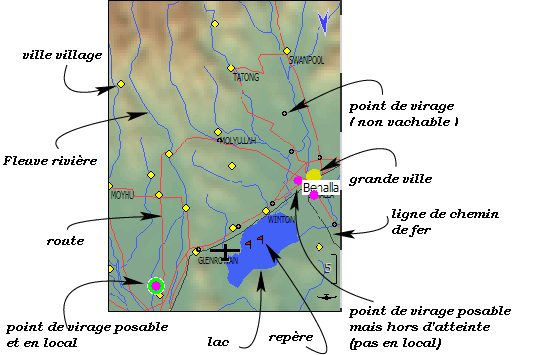
\includegraphics[angle=0,width=0.9\linewidth,keepaspectratio='true']{figures/fig-map.png}
\end{maxipage}

The moving map shows:
\begin{enumerate}
\item Glider, wind indicator, thermal profile, final glide indicator
\item Terrain, relief and hight of the terrain
\item Topography, rivers, roads, towns
\item Waypoints, airports, landabls
\item The active task, observation zones, turnpoints
\item The bearing (or route\footnote{The line to the next waypoint may be a
  {\em route}, as described in Section~\ref{sec:route}.}) to the next waypoint,
  heading
\item Airspaces
\item Markers, thermals history, snail trail
\item Glide range\footnote{The glide range is also referred to as the
  {\em reach}, as described in Section~\ref{sec:reach}.}
\end{enumerate}
The map is drawn in a projected coordinate system (not latitude and
longitude), and the scale can be changed (zooming in and out), as well
as panned.  All navigation functions take the curvature of the Earth
into account.

\section{Glider symbol, map orientation}
The glider symbol shows the position of the glider on the map.  The
orientation of the glider indicates the estimated heading of the
glider.

The map is oriented in one of three ways: North up,
Track up, or Target up.  Configuration settings \config{orientation} can be used
to specify a different map orientation when in circling mode. This is useful to prevent
disorientation when looking at the map while circling.  Target-up when
circling makes it easy to determine which direction to exit the
thermal.

When Track or Target-up is used in circling mode, the glider symbol is
centred on the screen, even if the symbol position is configured differently.
In cruise mode the Track and the Target-up orientation allows the glider
symbol to be positioned (e.g.) 20\% from the bottom of the screen, giving a good view of the
map ahead of the glider.  This position is adjustable in the configuration
\config{gliderposition} settings.

\section{Zoom and map scale}\label{sec:zooming}

To change the scale of the map, for PC, PNA, or Pocket PC:
\begin{enumerate}
\item Tap/click on a blank part of the map to highlight the map if it is not
already selected.
Then use mouse wheel, or the Pocket PC up/down key to either zoom
in or out.
\item A PNA with a button wheel let you also change the zoom.
\item Android devices have the +/- rocker that let you change the zoom.
\gesture{Up/Down}
\item You can also gesture to change the zoom level. Gesture
`{\it Up}' zooms in, `{\it Down}' zooms out.
\item Or select the function from the menu.
\begin{quote}
\bmenu{Display 1}\blink\bmenu{Zoom In} and \bmenu{Zoom Out}
\end{quote}
\item On Altair, the rotary knob can be used to zoom in and out.
\end{enumerate}

The map scale is displayed in the lower left corner of the moving map
display. The indicated distance is measured from the left to the right boarder
of the map display.
%\sketch{figures/zoom.png}
\marginpar{\includegraphics[angle=0,width=0.4\linewidth,keepaspectratio='true']{figures/zoom.png}}

Compaq Aero Users. If you enable the Compaq Aero Game Keys (On the
Q-menu) the centre two front buttons become the up/down keys.

There is a facility to have two zoom settings; one when the glider is
in circling mode, and one in the cruise or final mode.  This is the `{\it Circling zoom}'
option in the \config{circlingzoom} configuration settings.
By default, the circling zoom is set to about 2.5 km - 5.0 km, depending on the
display size. When the user zooms in or out, it affects the current
mode's zoom setting only, so when leaving the mode the previous mode's
zoom setting is used.  If `{\it Circling Zoom}' is not enabled,
there is only a single zoom level.

\marginpar{\includegraphics[angle=0,width=0.4\linewidth,keepaspectratio='true']{figures/zoomauto.png}}
`{\it Auto Zoom}' automatically zooms in when approaching a waypoint to keep
\menulabel{\bmenu{Display 1}\blink\bmenut{Zoom}{Auto}}
the waypoint at a reasonable screen distance. When `{\it Auto Zoom}' is active,
'AUTO' appears next to the map scale. The user can still zoom
in and out if desired, zoom will be switch to manual control automatically.

When a waypoint changes (automatically, via the task selector, or by
manually switching waypoints), `{\it Auto Zoom}' adjusts the zoom level
automatically so that the next waypoint is visible on the map.

During circling, if a thermal has been detected, then the map is centered about
the thermal or part-way such that the glider is still visible.

\section{Panning the map}\label{sec:panning}

A pan mode allows the user to explore areas beyond the glider.  This
is particularly useful when task planning.
\begin{enumerate}
\menulabel{\bmenu{Display 1}\blink\bmenu{Pan On}}
\item Enable pan mode by button menu, by gesture, or, on Android devices,
  by a two finger touch and swish over the map.
\gesture{Up - Right - Down - Left}
\item The map can then be panned by dragging the screen or using the cursor
  keys.  For Altair, panning is performed with the inner/outer rotary knob.
\item When done, pan mode has to be disabled manually, by pressing `{\it Pan Off}'
  from the special sub-menu of buttons in pan mode.
\end{enumerate}

\sketch{figures/pan.png}
When pan is active, the letters 'PAN' appears next to the map scale.  While
panning the location of the focus stays in the middle of the display under the
cross hairs.

Despite the focus under the cross-hairs (for Altair users) the map
still offers the `{\it What's here?}' feature just by touching any
position on the map (presuming a touch-screen).


\section{Waypoints} \label{sec:waypoint-schemes}
Waypoints are displayed with different symbols depending on the
waypoint type; the major distinction being landable and non-landable
waypoints.

\subsection*{Landables}
The waypoint symbols are drawn as shown below There are three icon sets for
landable waypoints. \config{waypointicons}

\begin{tabular}{c|ccc|ccc|}
Icon set
&\begin{sideways}Landable field\end{sideways}
&\begin{sideways}Marginal\end{sideways}
&\begin{sideways}Reachable\end{sideways}
&\begin{sideways}Airfield\end{sideways}
&\begin{sideways}Marginal\end{sideways}
&\begin{sideways}Reachable\end{sideways}\\
\hline
Purple Circle &

\includegraphics[width=0.8cm]{icons/winpilot_landable.pdf} &

\includegraphics[width=0.8cm]{icons/winpilot_marginal.pdf} &

\includegraphics[width=0.8cm]{icons/winpilot_reachable.pdf} &
\colorbox{white}{
\includegraphics[width=0.8cm]{icons/winpilot_landable.pdf}} &

\includegraphics[width=0.8cm]{icons/winpilot_marginal.pdf} &

\includegraphics[width=0.8cm]{icons/winpilot_reachable.pdf} \\
\hline
B/W &

\includegraphics[width=0.9cm]{icons/alt_landable_field.pdf} &

\includegraphics[width=0.9cm]{icons/alt_marginal_field.pdf} &

\includegraphics[width=0.9cm]{icons/alt_reachable_field.pdf} &
\colorbox[rgb]{0.94,0.94,0.94}{
\includegraphics[width=0.9cm]{icons/alt_landable_airport.pdf}} &

\includegraphics[width=0.9cm]{icons/alt_marginal_airport.pdf} &

\includegraphics[width=0.9cm]{icons/alt_reachable_airport.pdf} \\
\hline
Traffic lights &

\includegraphics[width=0.9cm]{icons/alt2_landable_field.pdf} &

\includegraphics[width=0.9cm]{icons/alt2_marginal_field.pdf} &

\includegraphics[width=0.9cm]{icons/alt_reachable_field.pdf} &
\colorbox{white}{
\includegraphics[width=0.9cm]{icons/alt2_landable_airport.pdf}} &

\includegraphics[width=0.9cm]{icons/alt2_marginal_airport.pdf} &

\includegraphics[width=0.9cm]{icons/alt_reachable_airport.pdf} \\
\hline
\end{tabular} \\

The {\it marginal} icons are drawn for those waypoints which are principally in the
reach, but it is not possible to approach them directly. E.g. a mountain prohibits a direct approach.

Waypoints are optionally labelled according to one of several
abbreviation schemes \config{labels} and visibility.

On top of this landable waypoints can be displayed more detailed. If
`{\it Detailed landables}' is switched on you get additionally information
encoded in the appearance of it's icon.
\begin{enumerate}
\item  Landable fields get a square-shaped icon despite what is shown in the table.
  The square is drawn like a diamond standing on one corner. Airfields stay with the
  circle shape, so that they become easy to distinguish.
\item  All icon sets, including the `Purple Circle' icon set, get the
  runway turned into their actual direction. The runway direction has to be available in
  the waypoint data. E.g. the SeeYou waypoint file format (\verb|.cup|) does
  include this information.
\end{enumerate}

XCSoar continually calculates which landing points are within gliding
range using the current wind estimate.  The estimated arrival altitude
{\em above the arrival safety height} of reachable landable points is
displayed next to the waypoint.  This arrival altitude is calculated
with the glider performance and MacCready setting configurable as
either that of the task\config{reachpolar}, or at a safety MacCready value.

\subsection*{Non-Landables}
As far as your waypoint file contains information on the nature of the
non-landable waypoints, the map will then display specific icons accordingly.
The table contains a collection of the currently supported map icons:

\begin{center}
\vspace{2.5cm}
\begin{tabular}{ccccccccc}
\begin{rotate}{60}Simple waypoint\end{rotate} &
\begin{rotate}{60}Mountain top\end{rotate} &
\begin{rotate}{60}Obstacle\end{rotate} &
\begin{rotate}{60}Pass\end{rotate} &
\begin{rotate}{60}Power plant\end{rotate} &
\begin{rotate}{60}Tower or building\end{rotate} &
\begin{rotate}{60}Tunnel\end{rotate} &
\begin{rotate}{60}Weather station\end{rotate} &
\begin{rotate}{60}Bridge\end{rotate}\\


\includegraphics[width=0.5cm]{icons/map_turnpoint.pdf} &
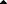
\includegraphics[width=0.8cm]{icons/map_mountain_top.pdf} &
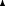
\includegraphics[width=0.7cm]{icons/map_obstacle.pdf} &
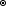
\includegraphics[width=0.7cm]{icons/map_pass.pdf} &
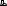
\includegraphics[width=0.8cm]{icons/map_power_plant.pdf} &
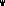
\includegraphics[width=0.7cm]{icons/map_tower.pdf} &
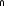
\includegraphics[width=0.6cm]{icons/map_tunnel.pdf} &

\includegraphics[width=0.6cm]{icons/map_weather_station.pdf} &
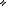
\includegraphics[width=0.8cm]{icons/map_bridge.pdf} \\

\end{tabular}
\end{center}


\section{Active task}

The active task course is drawn on the map as a blue (dashed) line.
Assigned area tasks also show the turn point sectors or areas as a yellow shaded
region.
Circles are always drawn around start and finish points, lines are
only drawn if the start/finish points are of line type.  Task
observation sectors are drawn as circle segments.

At all times a thick black line is drawn from the glider to the next
waypoint in the task.  This line may be the direct path to the waypoint,
or may be a {\em route} path clearing terrain and airspace obstacles, described in
further detail in Section~\ref{sec:route}.

\begin{center}
\begin{tabular}{c c c}
{\it Start/finish} & {\it Sector} & {\it Cylinder} \\
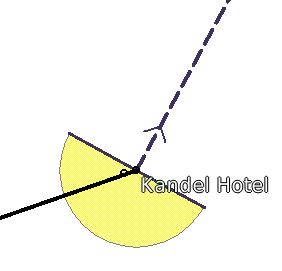
\includegraphics[angle=0,width=0.3\linewidth,keepaspectratio='true']{figures/cut-startfinish.png} &
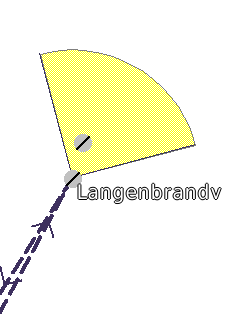
\includegraphics[angle=0,width=0.3\linewidth,keepaspectratio='true']{figures/cut-sector.png} &
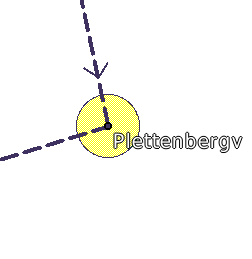
\includegraphics[angle=0,width=0.3\linewidth,keepaspectratio='true']{figures/cut-barrel.png} \\
\end{tabular}
\end{center}


\section{Terrain and Topography}\label{sec:terrain_topo}

The following topographical features are drawn on the map:
\begin{itemize}
\item Major roads, shown as red lines
\item Rivers, shown as blue lines
\item Large water bodies (lakes), shown as blue areas
\item Large cities, shown as yellow areas
\item Small population areas, shown as yellow diamonds
\end{itemize}
Cities and small population areas are labeled in italics.

Terrain is coloured according to elevation, and optionally shaded by sun, or
wind direction.  Invalid terrain, or terrain below
sea level is coloured blue.

\menulabel{\bmenu{Display 2}\blink\bmenut{Terrain}{On/Off}}
\menulabel{\vspace{1cm}\bmenu{Display 2}\blink\bmenut{Topo.}{On/Off}}

Terrain is shaded to improve visibility.  The default shading
is set up so that the virtual lighting position is the wind bearing,
thus brighter areas are on the upwind side of hills and dark areas in
the lee of the hill.
Support for a sun ephemeris is also implemented. If the slope shading is set
to `Sun', the brightness of a slope follows the day time in a very natural way.
The amount of shading and overall terrain brightness is configurable \config{shading}.

Both terrain and topography display can be switched on or off from the
menu.

\begin{tabular}{c c}
Topography & Terrain \\
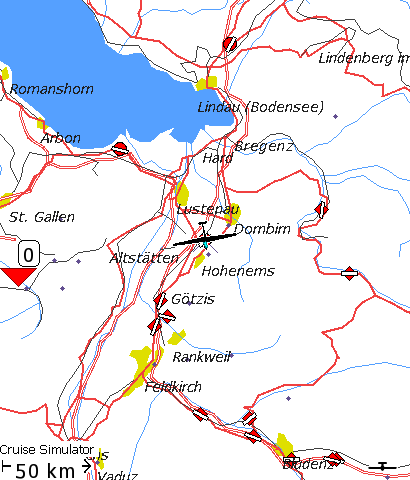
\includegraphics[angle=0,width=0.4\linewidth,keepaspectratio='true']{figures/cut-topo.png} &
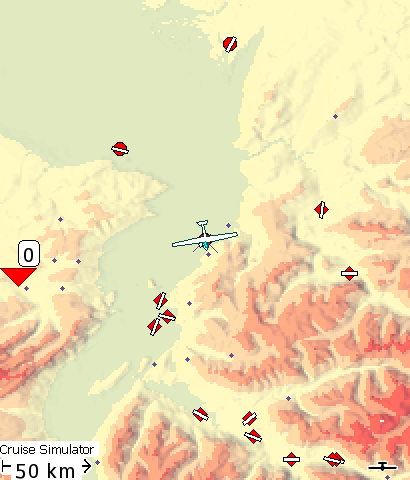
\includegraphics[angle=0,width=0.4\linewidth,keepaspectratio='true']{figures/cut-terrain.png} \\
\end{tabular}

If the terrain data is not available (or terrain display is turned
off), the background colour of the map window is white.  All terrain
below mean sea level is coloured blue.  If you are flying outside the
terrain region, the background colour will be white.

\subsection*{Map labels}\label{sec:maplabels}

The screen can be de-cluttered, turning off the display of topography
labels and non-task waypoint labels by toggling the `{\it Labels}' menu.
\menulabel{\bmenu{Display 2}\blink\bmenut{Labels}{None}}

Other options for display decluttering include:

\jindent{\bmenuth{Labels}{Task \&}{Landables}}{  Shows labels for the waypoints in
  the active task and any landable fields (based on the waypoint attributes in
  the waypoints file).  Other waypoints are shown but not labeled. }
\jindent{\bmenut{Labels}{Task}}{ Shows labels only for waypoints in the active task}
\jindent{\bmenut{Labels}{All}}{ Shows labels for all waypoints. }

Note that in all cases, the label format is configurable in the
`{\it Waypoint Display}' configuration menu.  \config{labels}


\section{Trail}\label{sec:trail}

An optional 'snail trail' is drawn on the map showing the glider's
path history.  The colour and thickness of the trail depends on the altitude or
on the variometer value.

\begin{center}
\includegraphics[angle=0,width=0.5\linewidth,keepaspectratio='true']{figures/snail.pdf}
\end{center}

If Vega or an intelligent variometer is connected with Netto output,
the Netto vario value is used; hence the colours and thickness of the
trail indicates the air-mass vertical movement rather than the glider's
vertical movement	.

\config{snailtrail}
The snail trail display can be toggled between {\bf Off}, a {\bf Short} trail
(about ten minutes), a {\bf Long} trail (about one hour) or a {\bf Full} trail
which displays the entire flight.  This can be performed permanently
through the configuration settings or temporarily by the
menu.
\menulabel{\bmenu{Display 2}\blink\bmenut{Trail}{Full}}

Note that for all of these modes, the snail trail is short in
circling mode in order to reduce screen clutter.

In order to assist centering thermals in the presence of wind, the
snail trail can be artificially drifted with the wind as it is
displayed (this is drift compensation).  In this way, the snail trail
is referenced to the prevailing wind rather than referenced to the
ground.  Since thermals drift with the wind also, the drifted trails
give a better indication of where the glider has been relative to the
thermals.

An example of this is illustrated below.  Note that when trail drift
compensation is active (right picture), the glider appears to be
circling in a column rather than an elongated spiral (left picture).

\begin{center}
\includegraphics[angle=0,width=0.6\linewidth,keepaspectratio='true']{figures/traildrift.png}
\end{center}

\config{traildrift}
Enabling trail drift compensation is performed through the
configuration settings.  The compensation is only performed
whilst in circling mode; the display of the trail in cruise mode is unaffected.
This can also be performed from the wind settings dialogue.
\menulabel{\bmenu{Config 1}\blink\bmenus{Wind}}

The trail drift display is useful also to show more clearly when thermals
are cranked due to wind shear.\\
The trail width can optionally be scaled according to the variometer display.

\section{Markers}\label{sec:markers}

Markers are shown as small flags (a) on the map.  The markers can be dropped
manually, by pressing a button, or automatically.  An example use of
automatic markers is to drop markers when entering circling mode, as a
simple way of showing all thermals encountered.

\menulabel{\bmenu{Nav 2}\blink\bmenut{Mark}{Drop}}
Markers are not preserved after XCSoar is exited, however the location
of all marks are appended to the file \verb|xcsoar-marks.txt|.

\section{Thermals}

While climbing in thermals automatically a mark is generated and stored up
\sketch{figures/thermalhistory.png}
to the end of the flight. This thermal history is accessible through the map
element functions in the same way as markers or waypoints.


\section{Glide range line}\label{sec:reach}

A reachable glide `footprint' is displayed on the map display as a
black and white dashed line, indicating where the glider would descend
through the terrain clearance height.  The reach shows clearance
tracks extending in all directions, optionally including paths around
terrain obstructions.  This feature is useful in assessing range with
respect to topography when searching low for lift, and when flying in
mountainous areas.

Reach calculations may be configured \config{turningreach} to two levels of detail:
\begin{description}
\item[Straight line] If turning reach is disabled, then the reach shows the
 furthest distance the glider can fly in final glide in all directions without
 turning.  This reach appears as a closed ring around the glider.

\begin{center}
\includegraphics[angle=0,width=0.8\linewidth,keepaspectratio='true']{figures/reach1.png}
% CUTOUT SHOWING GLIDE RANGE FOOTPRINT.  NO TOPOGRAPHY, FULLSCREEN, NO TASK. TURNING=FALSE
\end{center}

\item[Turning] If turning reach is enabled, then the reach shows the
  greatest area the glider can reach in all directions, even allowing
  turns around obstructions.\footnote{The maximum number of turns is
    set to three, and no turns may be greater than 90 degrees.}  The
  reach area appears as a closed ring around the glider but may also
  include holes indicating mountain peaks that the glider cannot reach
  without further climb.

\begin{center}
\includegraphics[angle=0,width=0.8\linewidth,keepaspectratio='true']{figures/reach2.png}
% CUTOUT SHOWING GLIDE RANGE FOOTPRINT.  NO TOPOGRAPHY, FULLSCREEN, NO TASK. TURNING=TRUE
\end{center}

\end{description}

The display can be configured to additionally blur the unreachable area
outside the glide range. \config{gliderange}
The final glide path is checked for whether the glider clears terrain along
the path by the terrain clearance height.  If clearance is not attained, a red
cross appears on the map at the point where the violation occurs. If a target is
defined the calculation is done along the straight path to the target. If no
target is defined the calculation is done along the current heading.

If reach is enabled, then the reachability of landable waypoints is used
by the abort task mode, alternate landable option lists and display of
landable waypoints on the map.

Note that task calculations are otherwise unaffected by reach
calculations --- for example, altitudes required as shown in the final
glide bar or task data as displayed in infoboxes do not take reach into account.

Furthermore, the reach calculations are used for footprint, landable
waypoint arrival heights, abort mode and the alternates dialogue.  The glider
performance and MacCready setting used in these calculations are configurable\config{reachpolar}:
\begin{description}
\item[Task] The MC value is that used in the task.
\item[Safety MC] A configurable, typically low MC value is set by the user to set
  performance near, but slightly degraded, to best glide performance. The amount of safety
  in the reach calculation is then the gap between best glide performance and the glide
  performance following the safety MC speed to fly.
\end{description}

\section{Status tabs `{\it Flight}' and `{\it Time}'}\label{sec:flight-status}

The status dialogue is a multi-tabular dialogue giving overview information on the
flight, system, task, rules and times.
It is accessed via the gesture "S", or with the button menu.
\gesture{Left - Down - Right - Down - Left}
\begin{quote}
\bmenu{Info 2}\blink\bmenu{Status}
\end{quote}

\subsection*{Flight}
Select the tabular page `{\it Flight}'.
The flight status dialogue shows the status of the aircraft's locality and can
be useful when giving position reports. It shows the location of the aircraft, the
maximum height gain, and nearest waypoint it's bearing and distance.
\sketch{figures/status-flight.png}

You may find this function useful when you need to report your
location to others.

\subsection*{Times}\label{sec:time-status}
Select the tabular page `{\it Times}'.
It shows the local time, flight time, takeoff and landing time and
the local sunrise, sunset times.

Note that the values in the Status dialogue
are static once the particular dialogue page is displayed.
\sketch{figures/status-times.png}
That is, position, times, etc. do not update while the page is displayed.
To see the updated values, it is necessary to select a different tabular,
then return to the previous dialogue to see the new values.


\section{Route}\label{sec:route}

XCSoar can plan paths around terrain and airspace obstacles in three
dimensions from the aircraft to the destination.  Such a path is known
as a route.  The height of the destination is the arrival height for
final waypoints, or may be higher for intermediate waypoints, as
dictated by the task system as required to complete the task.  Route
planning functions in normal ordered task mode, abort mode and goto
mode.

\begin{center}
\includegraphics[angle=0,width=0.8\linewidth,keepaspectratio='true']{figures/route3.png}
\end{center}

Routes take into account the glider polar performance and are
calculated to be optimal in the sense of minimum time.  By default,
route calculation is disabled, and can be enabled for terrain only or
terrain and airspace avoidance \config{routemode}.

Terrain is avoided vertically by the terrain safety height
\config{safetyterrain}, with no additional lateral clearance imposed.
Valid routes may result in the aircraft arriving at the destination
higher than the minimum height --- such as can occur when the
destination is just beyond a steep mountain.

Airspace is avoided horizontally by a buffer of approximately 250 m,
with no additional vertical clearance imposed.  Valid routes may fly
below or above airspace.

If MacCready is positive, then climbs are optionally allowed
 in the computed routes.  The top of the climb
may be limited to 500 m above the heigher of the start and destination
ceiling, or increased to the ceiling defined by the thermal ceiling
\config{routeceiling}.  Climbs above the higher of the start and
destination altitude are penalised by a slower climb rate than the
actual MacCready value.

Some approximations and limitations of the route planning system are as follows:
\begin{itemize}
\item Where climbs are necessary (and permitted) to reach the destination,
the climbs are assumed to occur at the start of the route.
\item Climb-cruise segments are assumed to occur at constant altitude,
equivalent to many small climbs distributed along the path.
\item Individual turns between path segments greater than 90 degrees
  are not permitted.
\item Failures of the solver result in the route reverting to direct flight
from the aircraft location to the destination.
\end{itemize}



%%%%%%%%%%%%%%%%%%%%%%
\chapter{Cross Country Tasks}\label{cha:tasks}

XCSoar provides a full task management system, in which tasks can be
edited prior to flight and, when undertaking casual cross-country
flying, modified during flight.  Waypoints are advanced automatically
or may be cycled through manually. Many of XCSoar's computations relate to
either turnpoints or the finish waypoint.
Unless a "true" task is defined, XCSoar will provide a "go home" function, with
many of the task related functions referring to the location of takeoff.
This chapter also describes the use of IGC loggers with XCSoar.

There are three task modes available:
\begin{description}
\item[Ordered task] This is the natural cross-country task type,
in which the task consists of a start point, zero or more waypoints,
and a finish point.  The task points are to be flown in order.
\item[Goto task] Flight to a single destination.
\item[Abort task] Provides options to fly to the nearest landing points.
\end{description}

Note that in goto and abort modes, the ordered task is retained and may be resumed
later, preserving any statistics about achievement in the task.

\subsection*{Automatic goto}

If no ordered task is defined, then on takeoff, a goto task is automatically
established with the takeoff point as the destination, or the nearest airfield
if it was close to the takeoff point.

Whether or not a task is defined, the takeoff point is always
generated and appears in the waypoint list for later reference or use.

After having defined an ordered task for the very first time, the automatic "goto takeoff" function is skipped. To resume a simple task, use goto.

\section{Goto tasks}

Goto tasks may be established by selecting a waypoint from the map,
the waypoint list, or any other mechanism e.g. the alternates dialogue,
and select \bmenuw{Goto}. In goto task mode, selecting
\bmenug{Nav 2}\blink\bmenug{Task Resume} resumes the ordered task (if
any).

\section{Editing tasks}

You can edit tasks in several ways.  Some methods are more useful for
editing prior to flight, and others allow tasks to be modified whilst
in flight for casual cross-country touring.  Tasks can be saved to
files and reloaded later, and can be transferred between any XCSoar
platform (Pocket PC, Altair, PC).

\tip It is also possible to save a `default' task and have this task loaded
automatically upon start-up of XCSoar.  One application of this is to
set up a default task with one waypoint being the home --- this means
that XCSoar is then programmed for final glide back to home, which is
useful for casual cross-country touring.

The main ways of setting tasks are the following:
\begin{itemize}
\item Using the task editor dialogue
\item Selecting waypoints from the map and adding them to the task from the
 waypoint details dialogue
\item Loading the task from a file
\end{itemize}

%Selecting the Task menu item will produce the Task dialogue box.  The
%list box on the left displays all of the turn points loaded into the
%system. Highlight the desired entries and using the "-$>$" and "$<$-"
%buttons assemble the desired task in the Task list box. As each turn
%point is added to the task a continuous display of the calculated task
%length is shown.  Tasks can be saved for recalling later using the
%"Save" button and recalled using the "Load" button.  Once the desired
%task is complete select "OK".
%
%{\it DIAGRAM SHOWING TASK DIALOG EDITING, WITH LABELED ARROWS POINTING
%TO THE USER INTERFACE ELEMENTS?}

Loading a task from file may be useful in competition or casual
cross-country flying in groups, as one person can distribute the task
file to others, thereby saving effort on editing the task severalfold.
\tip
If no task is present at startup, a task is created automatically,
containing one waypoint takeoff as ``goto home''.

XCSoar saves the current task when shutting down and loads it at
startup, thereby allowing the task to be entered early in the day,
then the device running XC Soar can be turned off until flight time.

Task waypoints are preserved even if the waypoint
file is changed.  This means, if you save a task, then change the
waypoint file, then load the task again, new waypoints are generated
for any waypoints that are missing in the new waypoint file.

\section{Waypoint Information}
%Several ways of selecting a waypoint are available:
%\begin{itemize}
%\item Touch its name or the waypoint symbol on the map screen if it is visible.
%\item If the waypoint is in the active task, highlight the waypoint {\InfoBox},
%  then use the up/down arrow keys to select the desired waypoint, and press the
%enter key.
%\item From the Task dialogue, find and highlight the waypoint in
% the waypoint list, then press the 'Details' button.
%\end{itemize}
%The display will now show the waypoint details dialogue.

The waypoint info dialogue describes a waypoint in detail and has
navigation functions such as GoTo, insert, append to the task, or set the
waypoint as the new home.
This may be accessed in several ways:

\gesturespec{rd}or menu \bmenug{Nav 1/2}\blink\bmenug{Task},
\todonum{descr. tabular "Turn Points"}
highlight a waypoint, then tap the highlighted waypoint again to display the
task point dialogue, then push \bmenuw{Details}.

\gesturespec{dl}or menu \bmenug{Nav 1/2}\blink\bmenug{Alternates}
to show the
details of the landables nearest to the aircraft.

\gesturespec{dr}or menu \bmenug{Nav 1/2}\blink\bmenug{Waypoint List}
, highlight and \bmenuw{select} a waypoint to show its details.

\gesturespec{urdl}or menu \bmenug{Display 1/2}\blink\bmenug{Pan On} to put the
map into pan mode, pan to the desired waypoint, touch its name or the waypoint
symbol.

\bmenug{Info 1/3}\blink\bmenug{What's here?}
to show the
item list under the cross-hair, or your index finger on the map.

The waypoint details dialogue contains two major pages (accessed via the
\bmenuw{$>$} and \bmenuw{$<$} buttons). Depending on the availability of further
details of the waypoint they will by shown on extra pages.

\subsection*{Waypoint details}\label{sec:waypointdetails}
This page contains text describing the waypoint's location, radio frequency and
runway information (if this information is in the waypoint file) elevation,
local daylight time, bearing and distance to the waypoint, and the altitude required
to reach the waypoint as described below. In addition, there is a button
\bmenuw{GoTo} to directly initiate
navigating to this waypoint. The button cancels the current task.
\begin{center}
\includegraphics[angle=0,width=0.8\linewidth,keepaspectratio='true']{figures/dialog-waypointdetails0.png}
\end{center}

As mentioned above, the Waypoint info dialogue also shows three forms of altitude
difference (additional
altitude required to reach the waypoint at the safety height) for
the corresponding waypoint:
\begin{description}
\item[Alt diff MC 0] Altitude difference at MC setting of 0
\item[Alt diff MC safety] Altitude difference at the abort/safety MacCready
  setting (see \ref{sec:safety-factor})
\item[Alt diff MC current] Altitude difference at the current MacCready setting
\end{description}

From the main Waypoint Info screen, you can access the second page by using the
\bmenuw{$>$} and \bmenuw{$<$} buttons in the bottom left corner of the page.
\subsection*{Task actions menu}
This page contains a column of buttons allowing various actions to be performed:
\begin{description}
\item[\bmenuw{Replace in task}] replaces the active waypoint in the task with
  the selected waypoint.
\item[\bmenuw{Insert in task}] inserts the selected waypoint before the active
  waypoint in
  the task.
\item[\bmenuw{Append to task}] adds the selected waypoint to the end of the task.
\item[\bmenuw{Remove from task}] removes the selected waypoint from the task.
  Note that this option is only visible if the selected waypoint is included in
  the active task.
\item[\bmenuw{Set as new home}] sets the waypoint as the home airfield.
\item[\bmenuw{Pan to waypoint}] switches to pan mode and pans to that waypoint.
\end{description}

It is a good idea to set your home waypoint from the waypoint details
dialogue. This causes XCSoar to start up at the home location regardless
of whether a GPS fix is received.  If no home is set, then XCSoar
starts in the centre of the terrain map.

\subsection*{Airfield information}
This page may contain relevant text from the enroute supplement about
the airfield, including runways, radio frequencies, traffic patterns,
contacts.
\begin{center}
\includegraphics[angle=0,width=0.8\linewidth,keepaspectratio='true']{figures/dialog-waypointdetails1.png}
\end{center}

\subsection*{Waypoint details image}
This page shows a satellite image of the waypoint.

\begin{center}
\includegraphics[angle=0,width=0.8\linewidth,keepaspectratio='true']{figures/dialog-waypointdetails2.pdf}
\end{center}
How to set up the detailed waypoint information read section \ref{sec:airfield-details}

\section{Waypoint selector dialogue}\label{sec:waypoint-selector-dialog}

The waypoint selector is a dialogue that allows waypoints to be easily selected
from a potentially large database. \gesturespec{dr}

Invoking the selector brings up a filtering dialogue screen with a set of
\menulabelr{\bmenug{Nav 1/2}\blink\bmenug{Waypoint List}}
optional filters on the left side of the page, and a list of waypoints on the
right, matching all of the filtering conditions set.
There are several filters available, which may be used together,
individually or not at all.
\begin{description}
\item[Name] Selects waypoints, starting with the string typed.
\item[Distance] Filters out waypoints farther than a specified distance from the
  aircraft.
\item[Direction] Filters out waypoints that are not in a specified direction
  from the aircraft.
  An additional special direction ``HDG(0°)'' filters waypoints within 30
  degrees to either side of the heading of the glider.  This allows the pilot
  to point the glider at a group of waypoints and quickly find them.
\item[Type] Filters out waypoints that are not of the specified type
(Landable point, Airport or Turnpoint) or that appear in the specified File~1 or
File~2 (primary or secondary waypoint file respectively).
\end{description}
When filtering by name and type, the list of matching waypoints is
sorted by name. When (in addition) filtering by distance or direction,
 the list of matching waypoints is sorted by distance.

\begin{center}
\includegraphics[angle=0,width=0.8\linewidth,keepaspectratio='true']{figures/dialog-waypointselect.png}
\end{center}

The list can be scrolled if there is more than one screen full of
matching waypoints.  To scroll through the list, simply drag with the finger, or
move to the bottom (or top) of the list with the cursor.

Selecting an item will result in different behaviour
depending on what function opened the waypoint selector.  In typical
use it brings up the waypoint details dialogue for the selected
waypoint.

\section{Task manager}\label{sec:task-manager-dialog}
\begin{it}  The task manager has undergone significant redesign compared with
earlier versions of XC Soar.\end{it}
\gesturespec{rd}

The task manager is used to edit, view, load, save to file, and declare cross
country tasks.
\menulabelr{\bmenug{Nav 1/2}\blink\bmenug{Task}}

The primary page is a calculator. It shows various calculations
related to the active task, as described in detail below.  In addition, there
are buttons for invoking dialogues \bmenuw{Turn Points}, \bmenuw{Manage},
and \bmenuw{Rules}, as well as a button to \bmenuw{Close} the task manager.

\subsection*{Task calculator dialog}\label{sec:task-calc-dial}
The task calculator dialogue allows the pilot to see the effect of
various changes to the task on final performance.
\menulabelr{\bmenuw{Calculator}}

In flight the Task Calculator might also be accessed from the Analysis pages.
With pages Task, Climb, and TaskSpeed a button \bmenuw{Task Calc} comes up,
that directly changes to the Task Calculator screen.


\begin{center}
\includegraphics[angle=0,width=0.8\linewidth,keepaspectratio='true']{figures/dialog-taskcalculator.png}
\end{center}

\begin{description}
%\item[Assigned task time]  This field displays the assigned task time.
\item[Estimated task time]  This field displays the estimated total time
  on task to complete the task at the provided MacCready setting.
\item[Task distance]  This field displays the task distance remaining.
\item[Set MacCready]  Allows the user to adjust the MacCready value and
  see the effect it has on the estimated task time.
\item[AAT range]  Allows the user to adjust the targets within the remaining
  AAT areas, to see the effect it has on estimated task time and task distance.
\item[Speed remaining]  This field displays the estimated speed for the
  remainder of the task at the provided MacCready setting.
\item[Achieved MacCready]  This field displays the achieved MacCready value.
\item[Achieved speed]  This field displays the achieved speed % at the achieved MacCready setting???
\item[Cruise efficiency]  100 indicates perfect MacCready performance, greater
than 100 indicates better than MacCready performance is achieved through flying
in streets. Less than 100 is appropriate if you fly considerably off-track. This
value estimates your cruise efficiency according to the current flight history
with the set MC value. Calculation begins after task is started.
\end{description}
See Section~\ref{sec:task-speed-estim} for more details on task speed
and achieved MacCready calculations.

On closing the dialogue the entered MacCready value is used as the MacCready
setting. If the \bmenuw{Cancel} button is pushed, the MacCready setting is
unaffected.

The \bmenuw{Target} button, for AAT tasks, adjusts the range
(increases or decreases) so that the estimated task time exceeds the
assigned task time by less than five minutes.  The range is adjusted
target-wise. In typical use, all targets are set to ``auto" that means the pilot
does not have to manually adjust the range to find the course for arrival at
the assigned task time, thereby reducing pilot workload.

\subsection*{Turn Points}
This page displays an ordered list of the points in the current active task.
\menulabelr{\bmenuw{Turn Points}}
If there are no waypoints in the active task, there
will be only an option to "Add Turnpoint."  By highlighting (tapping) the
"Add Turnpoint" function, then tapping in the highlighted region, the waypoint
selector is displayed, as described above.  Highlighting a waypoint from the
list and then tapping on the highlighted region adds the waypoint to the task.

\subsection*{Manage}
This page allows for invoking all operations needed to create new or manage
\menulabelr{\bmenuw{Manage}}already defined tasks.


\begin{itemize}
\item [\bmenuw{New Task}] Clears the current task and resets the task rules to
  the default values.
\item [\bmenuw{Declare}] If an external logger is connected, this will allow
  uploading the  active task to the logger and declaring it.
\item [\bmenuw{Browse}] Displays a list of all the saved tasks, allowing the
  pilot to load a previously saved task.  Note that this option will overwrite
  the current active task.
\item [\bmenuw{Save}] Saves the current active task.  Upon tapping the
  \bmenuw{Save} button the pilot will be prompted to enter a file name for the
  task to be saved.
\end{itemize}

\subsection*{Rules}
The values in the menu depend on the task type selected. Clicking any existing
\menulabelr{\bmenuw{Rules}} value will bring up another menu allowing the pilot to select a
different value for this rule.  Task types are discussed in more detail below.

Also, tapping on the \bmenuw{Rules} button again after it is highlighted allows
toggling between a "thumbnail" view of the task map and a larger view of the task.

\section{Task types}
XC Soar currently defines three different task types: Racing, AAT, and FAI badges/records.

A brief description of the task types is included below, but this manual does
not intend to rephrase FAI rules or contest task types. The reader is encouraged
to become thoroughly familiar with each task type by referring to contest rules
or FAI rules, which are available at \url{http://www.fai.org}.


\subsection*{Racing}
(also known as an "assigned task").  The racing task involves flight
around each specified turnpoint in the specified order.  Selecting the racing task
type allows the pilot to enter the following parameters.
  \begin{description}
  \item [Arm start manually] If set to ``On'', some extra buttons are presented
  in order to let you \bmenug{Arm start} as well as \bmenug{Disarm start} in
  menu \bmenug{Nav 1/2}, controlling  the detection of the start condition.
  \item [Start open time] This is the time when the start zone opens.
  \item [Start close time] This is the time when the start zone closes.
  \item [Start max. speed] This is the maximum speed allowed in the start observation
    zone.  This should be set to 0 if there is no limit.
  \item [Start max. height] This is the maximum height above the start height
    reference (AGL or MSL) at which a task can be started.  This  should be set to
    0 for no limit.
  \item [Start height ref.] This specifies whether the maximum start height is
    referenced to ground level of the start point ("AGL") or Mean Sea Level ("MSL").
  \item [Finish min. height] This is the minimum height based on the finish
    reference (AGL or MSL) at which a task can be finished.  This should be set to
    0 for no limit.
  \item [Finish height ref.] This specifies whether the minimum finish height
    is referenced to ground level of the finish point ("AGL") or Mean Sea Level ("MSL")
% \item [FAI start/finish rules] If enabled, this task type has no max. start height
%   or max. start speed.  Finish height reference is set to AGL and finish height
%   is 1000m below the start height \todonum[inline]{Is this description correct?}
  \end{description}

\subsection*{Assigned area task (AAT) and Modified area task (MAT)}
(also known as "Turn Area Task,"or TAT).  This is a task through assigned
areas (restricted to cylinder or sector observation zones).  A minimum task time
applies.  Rules options for this task type include:
  \begin{description}
  \item [AAT min. time]  This is the required minimum time for the task.  Refer
    to contest rules or consult an expert for penalties associated with finishing
    prior to the minimum time.  The time in this option is given in minutes.
  \item [other rules] All other rules stay the same as in case of task type
    ``racing''.
  \end{description}


\subsection*{FAI badges/records}
  \begin{description}
  \item [FAI start/finish rules] If set to ``On'', only start times might be set.
  If set to ``Off'', all other racing task rules might be altered from the FAI standard.
  \end{description}

Once the appropriate task type has been selected and start and finish rules
have been defined as described above, it is necessary to define the properties
of each waypoint in the task.

\section{Turn Points' task rules}\label{sec:task-rules}

The \bmenuw{Turn Points} dialogue brings up the list of waypoints in the task.
\menulabelr{\bmenuw{Turn Points}} If no waypoint is already defined, this screen
will show an empty list. With \bmenuw{(add Turnpoint)}, up and down arrows, and
\bmenuw{Make Finish} an ordered list of waypoints is created.
Waypoints can be start point, turnpoint, or finish point.
Highlighting any waypoint on the list and either tapping it again or
touching the \bmenuw{Edit Point} button brings up the waypoint definition.
Touching \bmenuw{Change type} will bring up a menu of the various task point
types available.  Definitions of each point type are given below.

A variety of task rules may be used when specifying tasks, including
the common FAI triangles and Assigned Area Tasks (AAT).  Many aspects
of the rules can also be customised.

Starting and finishing lines are centred on their associated waypoint
and aligned perpendicular to the next and previous waypoints
respectively.

Sector turn-points are 90 degree segments aligned to the bisection of
the previous and next waypoints, as commonly used in FAI tasks.
There is also support for British BGA, and German DAeC sectors.

\subsection*{Start point types}
The conditions to be met for a valid start depend on the type of start:
\begin{description}
\item[Start Cylinder] When the glider leaves the cylinder area.
\item[Start Line] When the glider crosses the start line.
\end{description}

\subsection*{Turnpoint types}
The conditions to be met for a valid turnpoint pass depend on its
 type:
\begin{description}
\item[FAI Sector] When the glider has entered the observation zone (OZ), defined
by a segment and radial distance from the waypoint.  The segment is
defined by a 90 degree arc centred about the bisector of inbound and
outbound legs, with a distance of 20 km.
\item[Keyhole Sector (DAeC 0.5/10 sector)] When the glider has entered the
observation zone, defined by a segment and radial distance from the waypoint.  The segment is
defined by a 90 degree arc centred about the bisector of inbound and
outbound legs, with a distance of 10 km.  The observation zone also includes
a cylinder of 500 m.
\item[Turnpoint Cylinder]  When the glider has entered the observation zone
defined by a radial distance from the waypoint.
\item[BGA Fixed Course Sector]  When the glider has entered the
observation zone defined by a segment and radial distance from the
waypoint. The segment is defined by a 90 degree arc centred about the
bisector of inbound and outbound legs, with a distance of 20 km.
The observation zone also includes a cylinder of 500 m (British rules).
\item[BGA Enhanced Option Fixed Course Sector]  When the glider has entered the
observation zone defined by a segment and radial distance from the
waypoint. The segment is defined by a 180 degree arc centred about the
bisector of inbound and outbound legs, with a distance of 10 km.
The observation zone also includes a cylinder of 500 m (British rules).
\item[Area Zylinder (AAT)]  and
\item[Area Sector (AAT)]  When the glider has entered the observation zone
defined by the radial distance from the waypoint, and segment for sector areas.
\end{description}

\subsection*{Finish point types}
Task completion depends on the finish type:
\begin{description}
\item[Finish Cylinder] When the glider enters the cylinder area.
\item[Finish Line] When the glider crosses the finish line.
\end{description}

Automatic advancement is triggered whenever a condition is met. To start an AAT,
mixed task, or Racing task the start has to be armed before.

\tip Competition rules may be defined in a profile file for
distribution to a group of pilots or task-setters, so all competitors
are playing by the same rules!

Additional task rules for valid starts and finishes may also be
specified.  Starts may have a defined maximum altitude above ground,
and a maximum speed.  Finishes may have a minimum altitude above
ground.  These parameters are defined in the page ``Default Task Rules'' in
the configuration \config{taskrules} settings.

For non-AAT tasks, an option is available to set the minimum finish
altitude according to the FAI rule, whereby the minimum finish
altitude is above 1000 meters below the start altitude.


%Need to add a section describing how to start the task%


\section{Advancing and restarting tasks}\label{sec:advanc-rest-tasks}
At all times one waypoint in the task is designated as the active
waypoint.  The active waypoint is used for calculation and display of
navigation information, that is, the pilot is directed to fly towards
the active waypoint (also referred to as the ``next waypoint'' in the
description of InfoBoxes as in Chapter~\ref{cha:infobox}).

During flight a continuous display of the bearing to the next waypoint is shown.

The altitude required to complete the task is calculated for the route starting
from the glider's actual position going through the task's turnpoints to the
final waypoint.

Changing the active waypoint is performed automatically, or may be performed manually.
The start point of racing tasks, and AAT task points, are special cases that require
the task point to be ``armed'' before the system will automatically advance to the next
task point once that point is reached.  All other task points will automatically
advance to the next point as soon as the last point was reached.

For non-racing tasks, no user interaction is required to
advance through the task --- the system will automatically advance as
each task point is achieved.  The user may still manually advance or retreat the active
task point by selecting the menu items \bmenug{Nav}\blink\bmenug{Previous turnpoint} and
\bmenug{Nav}\blink\bmenug{Next turnpoint} respectively.

The menu items \bmenug{Previous turnpoint} and
\bmenug{Next turnpoint} show dynamic labels that
indicate the action that will be performed upon selecting the item.

For task points requiring arming, \bmenug{Next Turnpoint} becomes
\bmenug{Arm turn} if the turn is not armed; if it is armed, then it becomes
\bmenug{Next Turnpoint} allowing for manual advance.
\bmenug{Previous Turnpoint} changes to \bmenug{Disarm turn} if the turn is armed
and vice versa. Similarly, for racing tasks these menu items update for arming
start points. If the Next Turnpoint is the \bmenug{Finish Turnpoint}, the menu
label changes accordingly.

Status messages are given for task points requiring arming, when
inside the observation sector, as reminders to arm the turn when the
pilot is ready to advance to the next waypoint. For starting, a
warning is given that the glider is in the start cylinder or behind
the start line, as a reminder to ``arm'' if necessary.

For PC and Pocket PC with touchscreen versions only, the user may
manually cycle through the waypoints by highlighting the waypoint
{\InfoBox} and by pushing the up or down cursor key.

See Section~\ref{sec:task-rules} for details on observation rules.

If a user has cycled through the waypoint manually, this does not mean
that the glider has successfully passed the waypoint!  However, this
facility is useful to force a task restart or to skip a waypoint when
flying a casual cross-country task.

\tip Tasks can be restarted simply by manually cycling back through the
waypoints to the start.

In all modes, if the glider re-enters the start zone or crosses the
start of the previous start, the task will be automatically restarted.

When selecting \bmenug{Previous turnpoint}, the trigger that detects
auto-advance for that waypoint is cleared; meaning that the task
manager expects the aircraft to fly to that observation zone (OZ)
again before continuing the task. The pilot may still select \bmenug{Next
turnpoint} to advance to the next task waypoint.

A system beep and message is given on task/waypoint advance.  The
messages are given when the system advances the task waypoint
automatically or, in manually arm mode, when the system is armed and the
aircraft is in sector:
\begin{description}
\item[Task start]  appears when the aircraft has crossed the start line or
 exited the start sector. This can be repeated any time.
\item[Next turnpoint]  appears when the aircraft has entered the observation
 sector for turnpoints. Turns with variable target advance as soon as
 \button{Arm Turn} is pushed.  For the manual arm mode, if the
 aircraft has already entered the observation sector and left, pushing arm will
 cause the task manager to expect, that the turn is intended to approach
 another time.
\item[Task finish]  appears when the aircraft has crossed the finish line
 or entered the finish cylinder.  This occurs in both advance modes.
\end{description}


\section{Alternate starts}\label{sec:alternate-starts}

%Alternate start points are skipped for XCsoar 6.0, but
%will potentially brought back in a next release.

%\todonum[inline]{Alternate start points are skipped for XCsoar 6.0, but
%will potentially brought back in a next release. This section can thus be
%treated as obsolete. }

The task system allows alternate start sectors to be defined:

\blink\bmenuw{Turn Points} select start point, \menulabelr{\bmenug{Nav 1/2}\blink
\bmenug{Task}}\bmenuw{Edit Point}\blink\bmenuw{Enable Alternate Starts}

On the start point edit page of the Task Manager turn on the \bmenuw{Enable
Alternate Starts} property. Another screen is brought up for defining an
alternate start point. In case, alternate start points have been defined before, label \bmenuw{Enable Alternate Starts} changes to \bmenuw{Edit Alternates}. After selecting ``Add Alternate Start'' and touching
\bmenuw{Relocate} the ``Select Waypoint'' filtering dialogue is invoked.

Having set up several alternate start points, the ``next waypoint'' scheme again will be extended. Before detection of a valid start and having armed start manually, the menu buttons stepping through all the waypoints will show label \bmenug{Next Start}.

Summarizing, all dynamic menu labels in menu \bmenug{Nav 1/2} show commands to be
executed for selecting waypoints and conditions either consecutively or in reverse
order.

%\begin{center}
%\includegraphics[angle=0,width=0.8\linewidth,keepaspectratio='true']{figures/%dialog-startpoint2.png}
%\end{center}

%  To edit the start points, move the cursor to an item in the list on
%  the right side of the dialogue, and press enter.  This opens the
%  waypoint selector dialogue, to allow selection of the waypoint.  This
%  process can be repeated several times for several alternate start
%  waypoints.  Press the `clear' button to clear all alternate start
%  points.

%  Each start sector is fixed to the same type (line/cylinder) and size
%  (start radius) defined in the task waypoint page.

%  Note that the task start point should be included in the alternate
%  start location list.

%\begin{center}
%\includegraphics[angle=0,width=0.8\linewidth,keepaspectratio='true']{figures/%dialog-startpoint3.png}
%\end{center}

%\begin{center}
%\includegraphics[angle=0,width=0.8\linewidth,keepaspectratio='true']{figures/%dialog-startpoint4.png}
%\end{center}

%  In flight, any time you cross a start line (or exit a start
%  cylinder), this will start the task at that particular alternate
%  start.  Task statistics are recalculated for the start sector you
%  last flew through.  All alternate start sectors are shown on the
%  map.  You can re-start simply by flying through the start sector
%  again or another start sector.  This automatic re-start will only
%  happen if the active waypoint is the first turnpoint after the
%  start, or the start itself.

%  When the waypoint advance mode is `Arm' or `Arm Start', then a start
%  is only recognised by XCSoar if the advance trigger is armed.

%  If desired, alternate start points may be selected as the active
%  waypoint by selecting the previous waypoint.  Continuing to select
%  the previous waypoint will cycle through all alternate start points.

\section{Abort/resume the task and Alternates}

If atmospheric conditions change for the worse, you may make the
judgement that it will be impossible to complete the task.  In this
situation, XCSoar can be instructed to ``abort'' the task, and it will
then help you reach a safe landing site. An ordered task can be aborted in
different ways. Either it is done by selecting a waypoint and execute the goto
command or by invoking the abort mode. In either case, the ordered task might be resumed.

\subsection*{Task Abort}\label{sec:taskabort}
Invoking the abort mode forces XCSoar to enter a special case of the final glide mode. \menulabelr{\bmenug{Nav 2/2}\blink\bmenug{Task Abort}} For a discussion on
flight modes refer to section \ref{sec:flightmodes}. In this flight mode
the configuration option `reach polar' determines whether
waypoint arrival heights in abort mode uses the MacCready value prior
to aborting the task, or if the safety MacCready value is used. \config{reachpolar}
Default is to use the safety MacCready value.  When switching to
abort mode, the MacCready setting is set to the safety value
if it is lower than the current setting.

With invoking abort mode the cross-country task is disabled. On the map radials
are drawn pointing to the nearest landables to instantly
support the pilot's decision. As is during the whole flight, the group of nearby
landables is maintained permanently. Radials and nearest landables may change
dynamically when in abort mode, so that at any time several landing options are
presented and any of these may be selected as the active waypoint. Even if no
landable is in reach, the radials are drawn.
\sketch{figures/abort-low.png}
If conditions improve, the task can be resumed by selecting the same
menu button that aborted the task, now denoting \bmenug{Resume Task}. The active
waypoint, prior to aborting the task, is then restored along with all the other
task details.

\subsection*{Alternates} \label{sec:alternates}
Alternates are maintained throughout the flight, reflecting good airmenship by
always keeping an eye on possible alternates.\menulabelr{\bmenug{Nav 1/2}\blink
\bmenug{Alternates}} Six landing
options are maintained. They are filtered by the configured ``alternates mode''
criteria (Simple, Task, or Home). \config{alternatesmode}
Choosing Task or Home puts some bias on the presentation of alternates to the
heading, you were taking whilst still task oriented.

As is with every waypoint list, additional information might be called by tapping \bmenuw{Details} before deciding which final to go. Select a waypoint from the list and push \bmenuw{Goto}.
\sketch{figures/alternates_list.png}

Although the items on the alternate list obey different rules they interact
in the same way
with the current task. Choosing a target from the alternates list aborts the task;
once the conditions get better the resuming of the task is doable by the already
mentioned button.


\section{Task status}\label{sec:task-status}

The status dialogue gives a summary of important task information.
\gesturespec{ldrdl} It can be useful to give a
good overview of the task status while freeing up InfoBoxes for other
purposes.  The status dialogue can be referred to in order to confirm
that a valid start was detected, as well as the progress against the
task.
\menulabelr{\bmenug{Info 2}\blink\bmenug{Status}}
The status dialogue can be invoked by menu or gesture left down right down left, denoting an S. The status tabs `Task' and `Rules' are of interest.

The task tab shows the AAT times, distances achieved and remaining and the
task speeds. The rules tab shows the validity of start/finish according
to the task rules.
\begin{center}
\begin{tabular}{c c}
Task & Rules \\
\includegraphics[angle=0,width=0.4\linewidth,keepaspectratio='true']{figures/status-task.png} &
\includegraphics[angle=0,width=0.4\linewidth,keepaspectratio='true']{figures/status-rules.png} \\
\end{tabular}
\end{center}

\section{Assigned Area Tasks}\label{sec:aat-tasks}

\subsection*{AAT targets}

A {\em target} is a point within an AAT area that the pilot intends to
fly to.  These targets can be moved within the AAT areas so the pilot
can adjust the effective distance of the task.  Targets may be set on
the ground, during task planning, and modified during flight.

When flying an AAT task, the navigation system directs the glider to
the target, and statistics like distance to waypoint are also relative
to the target rather than the waypoint of the AAT area itself.

Automatic task waypoint advancement does not trigger when entering an
AAT area solely. The pilot has to arm the turn manually to advance to the next
turn. When arming the AAT turn while flying through the OZ also the task
optimiser is triggered to capture the realized AAT target and bring the target
optimisation for the rest of the task up to date. See Section~\ref{sec:advanc-rest-tasks}
for details.

\subsection*{Manually moving targets}

In order to make the specification of targets more straightforward,
their location is defined by a range parameter that determines how
far from the minimum to maximum possible distance the target is.  This
is expressed as a percentage.  For example, with range set to 100\%,
the target is located to give the maximum overall task distance.  With
range set to~$-100$\%, the target is located to give the minimum overall
task distance.

Zero range yields a nominal task distance: for sectors the target is
half way along the bisector radial; for cylinders the target is in the
center of the cylinder.

The task calculator dialogue (see Section~\ref{sec:task-calc-dial}), shows the
average percentage over all turns in the AAT Range field.
The targets can be individually modified from the target dialogue of the task
calculator.


\subsection*{AAT targets and the Task Calculator}

The typical use of targets in flying AAT is as follows:
\begin{itemize}
\item Set the expected MacCready, bugs/ballast and wind settings
  for the flight using the flight settings and wind settings dialogues.
\item Define the task as normal from the task editor.
\item Based on the pilot's judgement of how good the weather is,
  and whether some areas are likely to be more or less difficult than
  others, targets may be set individually for each turn-point in the
  target view.  The ETE field in the target view compared to
  the assigned minimum time is shown as Delta T to check if the planned
  task is efficient and long enough.
\item During flight, if situations change, such as changed MacCready setting
  or wind, the task calculator can be brought up to show the estimated
  task time, again allowing comparison to the assigned minimum time.
\item If the pilot decides to extend or shorten the flight, all the remaining
  targets can be modified from the task calculator.
\end{itemize}

The task calculator therefore allows the pilot to make (and help to
answer) `what if?' questions, for example:
\begin{itemize}
\item What will happen if the conditions improve?  The MacCready setting can be
increased and the pilot can see if there is sufficient adjustment to targets in
order to be able to extend the planned task.
\item What will happen if the conditions deteriorate?  The MacCready setting can
be decreased and the pilot can see how much the task can be shortened and still
finish the task later than the assigned minimum time.
\item What will happen if I leave the AAT area now?  By pressing \button{Arm
turn} the take over of the current position into the optimization can
be forced. The repositioning of subsequent turns can be reviewed in the task calculation
dialogue.
\end{itemize}

\subsection*{Target projection}

XCSoar continually analyses the path of the glider through AAT sectors
to find the points in previous AAT sectors through which the achieved
scoreable distance will be greatest.  Internally, the program moves
the targets for previous AAT sectors, which are then the optimal
targets.

In certain conditions, targets for the current AAT sector may be moved
automatically:
\begin{itemize}
\item When inside an AAT sector, the target in that sector is moved to
to a line projecting from the previous sector's target through the
aircraft, at the same distance from the previous sector's target to
the target prior to entering the sector.  The effect of this is to
allow pilots to choose to enter an AAT sector in a different direction
or offset from the direct line from the previous target to the current
target.

\item While the aircraft is in the AAT sector and the distance from the
previous target to the aircraft is greater than the distance from the
previous target to the current target, the target is moved further
along the projected line from the previous target to the aircraft,
just beyond the aircraft.  Hence, the black track line will not be
visible but the blue optimal track arrow will point along this
projected direction.
\end{itemize}

A worked example is provided in the following figures to illustrate
how targets move during a flight and to show how XCSoar determines the
maximum scored path.

\begin{maxipage}
\begin{center}
\begin{longtable}{|c|c|}
\toprule
\includegraphics[angle=0,width=0.45\linewidth,keepaspectratio='true']{figures/faat01.png} &
\includegraphics[angle=0,width=0.45\linewidth,keepaspectratio='true']{figures/faat02.png} \\
{\em Outside sector} & {\em Inside sector} \\
Target (-20\%) is on bisector & Target moved along track line \\

\midrule
\includegraphics[angle=0,width=0.45\linewidth,keepaspectratio='true']{figures/faat03.png} &
\includegraphics[angle=0,width=0.45\linewidth,keepaspectratio='true']{figures/faat04.png} \\
{\em User decreased range} & {\em User increased range} \\
Target (-80\%) moved along track line & Target (80\%) moved along track \\

\midrule
\includegraphics[angle=0,width=0.45\linewidth,keepaspectratio='true']{figures/faat05.png} &
\includegraphics[angle=0,width=0.45\linewidth,keepaspectratio='true']{figures/faat06.png} \\
{\em Analysis (task page)} & {\em Next waypoint} \\
Path around active target  & ``Arm Turn'' pressed \\
\bottomrule
\end{longtable}
\end{center}
\end{maxipage}

\begin{maxipage}
\begin{center}
\begin{longtable}{|c|c|}
\toprule
\includegraphics[angle=0,width=0.45\linewidth,keepaspectratio='true']{figures/faat07.png} &
\includegraphics[angle=0,width=0.45\linewidth,keepaspectratio='true']{figures/faat08.png} \\
{\em Analysis (task page)} & {\em Approaching next area} \\
Best scored target found & Target (60\%) is on bisector \\

\midrule
\includegraphics[angle=0,width=0.45\linewidth,keepaspectratio='true']{figures/faat09.png} &
\includegraphics[angle=0,width=0.45\linewidth,keepaspectratio='true']{figures/faat11.png} \\
{\em Inside sector} & {\em Next waypoint} \\
Target (60\%) moved along track line & ``Arm Turn" pressed \\

\midrule
\includegraphics[angle=0,width=0.45\linewidth,keepaspectratio='true']{figures/faat12.png} &  \\
{\em Analysis (task page)} &  \\
Best scored targets found &  \\

\bottomrule
\end{longtable}
\end{center}
\end{maxipage}

\section{OnLine Contest}

The analysis dialogue contains a page `OnLine Contest' which can be
used to show the optimal path and estimated score.  The configuration settings \config{taskrules}
(task rules page) allows the selection of which set of rules to be used for the
OLC optimisation.

The optimization is done continuously in the background and can be retrieved at
any time. The analysis page shows a graphical overview of the optimisation
result besides distance and score. A InfoBox is available which gives the
instant OLC distance and score as well.

\begin{center}
\includegraphics[angle=0,width=0.8\linewidth,keepaspectratio='true']{figures/shot-olc.png}
\end{center}

When flying OLC, either AAT or non-AAT tasks may still be used to
manage the flight navigation.  During flight, the computer will optimise the
current flight with respect to the selected OLC rules.

In the OLC analysis page, the aircraft track is shown as a thin green line, the optimal
path is shown as a thick red line.

The score and computed optimal distance is approximate.

When the aircraft has landed, the displayed result gets not updated anymore.


\section{Logger}\label{sec:logger}

A flight logger conforming to the IGC file specification can be used
to record flights.

Several flight loggers are accessible via XCSoar:
\begin{itemize}
\item A software-based logger.  All versions of XCSoar have this
  functionality.  The logger conforms to the IGC standard but is not
  certified.
\item For example the PRO version of Altair has an internal IGC certified logger
  device.  XCSoar communicates with the logger as to any other external device.
\item XCSoar can also send declarations to some external logger devices.
  For this to work, the device must be specified in the `Devices'
  section of the configuration \config{comdevices} settings.
\item  For some of the numerous logger devices XCSoar can download IGC files.
  This is convenient especially for logger devices, which are not that easy
  removable from the glider.
\end{itemize}

\subsection*{Setup}
For a complete matrix of the supported logger features see section~\ref{sec:supported-varios}.
The configuration is described in detail in section~\ref{conf:logger}.  Details
to the log files can be found in section~\ref{sec:logfiles}.

\subsection*{Logger activation}
The logger can be turned on and off automatically or manually.  For para-glider
XCSoar provides the option to only start the logger automatically. Thus a very
slow and close to the terrain flight won't automatically stop logging the flight.
If you choose the auto start only logger you have to stop the logger manually.
To turn the logger on (or off) manually, select from the menu:
\sketch{figures/logger-startdeclare.png}
\begin{quote}
\bmenug{Config 3}\blink\bmenut{Logger}{Start}
\end{quote}

When the internal software logger is active, a small `green status led' in the
lower right corner of the map area flashes once per second.

By default, XCSoar is set up to automatically start and stop the
internal software flight logger when it detects the aircraft is flying
and when it has landed, respectively.  Only when the logger is
manually started does it ask if the flight is to be declared; when
automatically starting it automatically declares the current task.
In simulation mode the logger does not get activated automatically.

If a task has been declared, then subsequent attempts at modifying the
task result in a warning message asking to confirm whether the action
is to be taken and invalidate the declaration.  This is intended to
make it harder to accidentally modify the task resulting in a failed
declared task.

The XCSoar software logger, when started, checks for 500kB of free
space on the file storage.  If there is insufficient space, it will
automatically delete IGC files, oldest first, in order to free up
500kB.  It does not ask the user for confirmation before performing
this operation. \warning

The internal software logger buffers data so that when it starts
(automatically or manually) up to 60 seconds of data prior to starting
is recorded.  This means that the software logger now adequately
captures the full take-off.

\subsection*{Logger replay}\label{sec:logger-replay}
Flight logs in the IGC format generated by XCSoar or other loggers can
be replayed.  The logger replay dialogue can be accessed via the
menu:
\begin{quote}
\bmenug{Config 2}\blink\bmenug{Replay}
\end{quote}
\sketch{figures/loggerreplay.png}

During replay, the word `REPLAY' appears at the lower left corner of
the screen.  During replay, the program behaves as if real GPS updates
are being received by a GPS.  The logger replay dialogue does not need
to be open during replay.

To start a log replay, first select the file to load, and then select the
\button{Start} button.  The replay can be performed in accelerated time
by changing the time scale from 1x to a higher number, and paused by
setting the time scale to zero.  High time scales can result in degraded
performance of the wind estimation and other statistics/analysis routines.

Stop the log using the \button{Stop}.
Once a log is started, further presses of the \button{Start} has the
effect of restarting the replay.

\tip It is recommended to reset the device before flight, after a log
file has been replayed, in order to ensure that XCSoar's internal
statistics are properly reset.

When operating XCSoar in FLY mode, the replay is disabled (stopped) if
the real GPS receiver detects that the aircraft is moving.

The logger replay works best with high sampling rate log files;
a 6 second interval or less works fine.

\subsection*{Error analysis logger}\label{sec:raw-logger}
For the pure reason of tracking down error prone behaviour of XCSoar
there is a `Raw Logger'. In case you are able to reproduce an error you can
activate the raw log file creation by:
\begin{quote}
\bmenug{Config 3}\blink\bmenug{Raw Logger}
\end{quote}
Developers will appreciate very much any detailed error description including a log file like this. It really facilitates the root cause analysis and saves time to fix an error.

\section{Flight analysis} \label{sec:analysis-climb}

The analysis dialogue is very useful in planning and conducting
cross-country flights.  It is accessed via the menu:  \gesture{Up - Right - Down}
\begin{quote}
\bmenug{Info 1}\blink\bmenug{Analysis}
\end{quote}

Several pages are of interest:
\begin{description}
\item[Barograph]  Shows a graph of the history of the altitude of the glider.
  Statistics are used to estimate the thermal working band (average
  base and ceiling of climbs) and to estimate how the ceiling is
  changing over time.  The base and ceiling lines are drawn on the
  barograph.

  The `Settings' button opens the flight settings dialogue
  (e.g.\ to adjust the QNH)

\begin{center}
\includegraphics[angle=0,width=0.8\linewidth,keepaspectratio='true']{figures/analysis-barograph.png}
\end{center}

\item[Climb history]
  Shows a bar chart of the average climb rate achieved during each
  climb.  Statistics are used to estimate the overall average climb
  rate, and to estimate how this average is changing over time.  The
  current MacCready setting is drawn on the bar chart as a thick red
  dashed line, and the climb rate trend is drawn on the chart as a
  blue line.

  The ``Task Calc'' button opens the task calculator,
  (e.g.\ to adjust the MC value)

\begin{center}
\includegraphics[angle=0,width=0.8\linewidth,keepaspectratio='true']{figures/analysis-climb.png}
\end{center}

\item[Task]
  This page shows an overview of the entire task.  The main task line
  is drawn in thick dashed green, AAT areas are shaded.  For AAT
  tasks, the path from the aircraft around the remaining targets within AAT
  areas is shown in red.  The aircraft track is shown as a thin green line.

  The `Task Calc' button opens the task calculator,
  (e.g.\ to adjust the AAT task range or MC value)

\begin{center}
\includegraphics[angle=0,width=0.8\linewidth,keepaspectratio='true']{figures/analysis-task.png}
\end{center}

\end{description}

\section{Sunlight and time}

A sun ephemeris computes the time of sunrise and sunset, which is displayed in the
Aircraft Status dialogue (see Section~\ref{sec:time-status}).  Note that
local terrain and atmospheric conditions may result in poor visibility
before the displayed sunset time.

For PDA systems, the clock is adjusted for daylight saving time according
to the settings in the operating system.  For Altair, the clock UTC offset
must be adjusted manually for daylight saving time in the configuration
settings dialogue.

If the expected arrival time at the final waypoint in the task is past
sunset, a status message warning is issued.


%%%%%%%%%%%%%%%%%%%%%%
\chapter{Glide Computer}\label{cha:glide}
This chapter focuses on how XCSoar's glide computer works and is
recommended reading so you understand the specific details of
calculations being performed and how to use the software properly.  It
assumes a basic knowledge of cross-country soaring, but is suitable
reading for competition pilots as well as pilots engaging in casual
cross-country touring.

\section{Flight modes} 
XCSoar performs different calculations and may dispay different
InfoBoxes depending on the flight mode, for example Circling
(thermalling), Cruise, or Final Glide (cruise to the Finish waypoint).
XCSoar automatically detects the difference between thermal (circling)
flight and cruising flight. After about 30 seconds of circling flight
the software will switch from cruise to climb mode. After about 30
seconds of straight line flight the software will switch from climb to
cruise mode.

The cruise modes are further divided into final glide and normal
cruise.  Final glide is active when the last waypoint in the task is
active, or when the task is in abort mode.

Switching between the different flight modes is automatic.  Circling
is enabled when the glider turns (typically three quarters of a turn).
It is possible to have circling mode switched based on an external
input (e.g.\ from a pilot-operated switch).

A small symbol is drawn on the lower right corner of the map area to
indicate which flight mode the computer is in.

\begin{tabular}{c c c c}%{c c c c}
\includegraphics[angle=0,width=0.75cm,keepaspectratio='true']{icons/mode_cruise.pdf} &
\includegraphics[angle=0,width=0.75cm,keepaspectratio='true']{icons/mode_climb.pdf} &
\includegraphics[angle=0,width=0.75cm,keepaspectratio='true']{icons/mode_finalglide.pdf} &
\includegraphics[angle=0,width=0.75cm,keepaspectratio='true']{icons/mode_abort.pdf}\\
(a) & (b) & (c) & (d)
\end{tabular}

\begin{description}
\item[Cruise (a)]   The glider is not circling and there is either no task
  active, or the task waypoint is not the finish point.
\item[Circling (b)]  The glider is circling (though it may not be climbing).
\item[Final glide (c)]  The glider is not circling and the active waypoint is the
 final one in the task.
\item[Abort (d)]  This manually-triggered mode indicates the immediate landing
options to the user.(see Section~\ref{sec:abort-resume-task})
\end{description}

The specific computations performed by XCSoar are of course dependent
on this flight mode.  The display changes in each mode, principally,
the InfoBoxes may be set up differently for each mode; secondly there
is a facility to automatically change zoom between circling and other
flight modes (this is called `circling zoom').

In addition to these display modes, an auxiliary set of InfoBoxes may
be displayed in any flight mode.  This is useful if the pilot has
information he wants to be able to view no matter what mode the
computer is in.  This is accessed from the menu
\begin{quote}
\bmenu{Info ..}\blink\bmenu{Aux Info On}
\end{quote}

which toggles between the normal mode-specific InfoBoxes and
the auxiliary set of InfoBoxes.

Final glide mode replaces the Cruise mode as soon as the glider is
above the final glide path. The required height depends most
importantly on the adjusted MC value, but also the ground clearance is
considered. On entering a thermal while in Final glide mode XCSoar
will switch to the Circling display and back to the Final glide
display once the thermal is left again and the final glide condition
is still met (i.e. the glider is still above the final glide path,
considering MC setting and terrain). The potential of having the Final
glide mode is obvious when flying short tasks in which the aircraft
may well be above final glide turning the penultimate waypoint.

\section{MacCready setting}

The MacCready setting may be adjusted several ways:
\begin{itemize}
\item From the menu items
\begin{quote}
\bmenu{Config}\blink\bmenu{MC $+$/$-$}
\end{quote}

\item For touchscreen/mouse devices, select the MacCready InfoBox field, then
  use the up and down arrow keys.
\item When connected to a supported intelligent variometer, adjusting
  the MacCready setting on the variometer will change the setting
  in XCSoar according to the devices synchronisation configuration (see 
  section~\ref{conf:comdevices}).
\end{itemize}
In addition, an automatic MacCready mode is available as described in
Section~\ref{sec:auto-maccready}.

\section{Glide polar}

The glide polar specifications of a wide selection of glider types,
representing major classes of gliders, are built into XCSoar.
If your glider type is not listed, these may be used as an approximation for  
if no better glide polar can be found.  However, for most accurate results, it is
advisable to use the correct glide polar for your particular
\config{polar} aircraft type. 

The glide polar is adjusted in flight by XCSoar to account for
degraded performance due to bugs and ballast.

The build-up of bugs on the wing's leading edge, as well as rain
droplets on the wing, affect the aerodynamic performance.  It is the
pilot's responsibility to judge and update the bugs value during
flight.  The bugs value is expressed as a percentage of the clean
glider's performance.  For example, at 100\% bugs value (left side), the glider
performs as a clean glider, and at 50\% bugs value (right side), the glider's
sink rate is doubled when compared to a clean glider. 

\begin{center}
\includegraphics[angle=0,width=\linewidth,keepaspectratio='true']{figures/cut-clean-dirty-polar.png}
\end{center}
Knowing all this, a meaningful setting for a worst-case bug polluted wing could
scale down the polar by 30\% to 70\%. Some experimentation may be required to determine appropriate settings for bugs, because the performance degradation experienced by different glider types may be different.

The ballast value is expressed as a percentage of the glider's total
ballast capacity.  Depending on the specific construction of the glide
polar file, this may optionally include a weight margin to provide for
different pilot weights.  When flying with no ballast, a heavy pilot
may set a ballast value of perhaps 10\% so that the polar is
appropriately adjusted for the increased cockpit weight.

%{\it DIAGRAM SHOWING GLIDE POLAR, 0\% BALLAST AND 100\% BALLAST}

The current glide polar and all up weight can be reviewed in the
analysis dialog as described later in this chapter.

\section{Flight setup dialog}\label{sec:flight-setup}
Use the flight settings dialog to modify the all up weight of the glider both
before and during flight, as well as to set the QNH pressure.  

This is accessed via the menu under 
\begin{quote}
\bmenu{Config}\blink\bmenu{Flight Setup}
\end{quote}

\begin{center}
\includegraphics[angle=0,width=0.45\linewidth,keepaspectratio='true']{figures/dialog-basicsettings.png}
\end{center}

The bugs setting ('clean') determines the amount the polar is degraded
due to contamination during a long flight.  A 'clean' setting of 100\%
will cause the software to use the clean polar. A 'clean' setting of
50\% will degrade the polar by 50\%, effectively doubling the sink
rate for a given airspeed.

The ballast setting is used to modify the polar to account for any
water ballast carried during the flight. Ballast is shown in liters,
and should be set to correspond to the correct water ballast added
before flight.  The ballast setting modifies the polar to account for
the indicated load of water ballast.

Use this dialog both before and during the flight to record the mean
sea level atmospheric pressure, also known as QNH pressure.  The
software uses the values entered to convert airspace flight levels
into altitudes.  If connected to a supported intelligent variometer
with an altimeter, the altitude is updated on this dialog as the QNH
pressure is adjusted.  This makes it easy to set the QNH pressure if
the airfield elevation is known.

The maximum forecast ground temperature is used by the convection
forecast algorithm (see Section~\ref{sec:convection-forecast}) in its
determination of estimated convection height and cloud base.

\tip It is possible to configure XCSoar to display the basic
settings dialog when it starts up.

On system startup, after the GPS has acquired lock, and if a
barometric altitude source is connected (e.g.\ Vega, AltairPro,
FLARM), the QNH is automatically adjusted.  This adjustment sets the
QNH such that the barometric altitude equals the terrain altitude.

The QNH is only updated if the aircraft is on the ground for more than
10 seconds, so that if XCSoar is restarted during flight, QNH will not
be adjusted.  The update only occurs also if the terrain database is
valid at the current aircraft location.

\section{Speed command display}

When used in conjunction with an intelligent variometer that produces
indicated airspeed measurements, a speed command chevron is drawn
on the right side of the map display.  If the glider is flying slower
than the optimal speed, the chevrons are red and point downwards.  If
the glider is flying faster than the optimal speed, the chevrons are
green and point upwards.  If the speed is approximately optimal, no
chevrons are drawn.

%{\it DIAGRAM SHOWING SPEED COMMAND CHEVRONS}

Depending on the configuration, speed command chevrons can be
displayed on the right side of the map area, or on the variometer
gauge.

\section{Speed to fly}\label{sec:stf}

XCSoar continuously calculates two types of speed to fly:
\begin{description}
\item[MacCready speed]  This is the best speed to fly during cruise
  in still air, adjusted for wind if in final glide mode.
\item[Dolphin speed]  This is the instantaneous, best speed to fly
  in rising or descending air, adjusted for wind if in final glide
  mode.
\end{description}  

The user can specify a maximum manoeuvring speed in the configuration
settings, which limits the speed-to-fly in MacCready calculations to
realistic values.

Different pilots have personal preferences as to whether they prefer
to fly in so-called `block MacCready' style, in which they fly
constant speed between thermals according to the MacCready speed; or
to fly in `dolphin' style, in which they fly at varying speeds
according to the continuously changing Dolphin speed value.

\begin{maxipage}
\begin{center}
\includegraphics[angle=0,width=0.8\linewidth,keepaspectratio='true']{figures/figure_speed_to_fly.pdf}
\end{center}
\end{maxipage}

A configuration option `Block speed to fly' (see
Section~\ref{sec:final-glide}) can be used to specify whether dolphin
or block speed to fly is used.  The infobox `V Opt' shows the optimum
speed according to whichever mode is selected.  When connected to the
Vega intelligent variometer, the speed command sounds are based on
this optimum speed value.

\section{Speed to fly with risk}\label{sec:speed-fly-with}
  The speed to fly system can be compensated for risk, in which the
  MacCready setting used for calculating the speed to fly (in both
  Block or Dolphin modes) is reduced as the glider gets low.

  Many pilots typically wind down the MC as they get low --- this
  feature performs this automatically.  The theory governing how this
  is implemented in XCSoar is based loosely on the paper by John
  Cochrane, ``MacCready Theory with Uncertain Lift and Limited
  Altitude'' {\em Technical Soaring} 23 (3) (July 1999) 88-96.

\url{http://faculty.chicagogsb.edu/john.cochrane/research/Papers/newmcred.pdf}

  A configuration parameter $\gamma$ (`STF risk factor', in the
  configuration settings under page `Glide Computer') controls how the
  risk MC value is calculated.  The $\gamma$ factor determines the
  fraction of the current MacCready setting as a function of the
  height fraction.  The height fraction used in this calculation is
  the ratio of the height above terrain ($h$) to the height of the
  maximum climb (this will usually be close to cloudbase) above the
  terrain ($h_{top}$).  The $\gamma$ setting thus represents the
  fraction of the total available climb (cloudbase minus terrain) at
  which you would wish to abandon the task and begin to prepare for a
  landout.  Thus, low $\gamma$ values indicate a higher tolerance for
  landout risk than higher values of $\gamma$.

  For the default value, $\gamma=0.0$, there is no compensation ---
  the risk MC is the same as the MC setting.  For $\gamma=1.0$, the
  risk MC is scaled linearly with the height fraction $h/h_{top}$.
  For intermediate values of $\gamma$, the risk MC varies smoothly
  with the height fraction, such that the risk MC is small only when
  low.

  Low values of $\gamma$ are best when pilots do not want to slow down
  as they get low (but risk out-landing); high values of $\gamma$ can
  be used for very cautious pilots but will result in lower average
  speeds.

  A value of $\gamma=0.3$ is recommended.

\begin{center}
\includegraphics[angle=0,width=\linewidth,keepaspectratio='true']{figures/riskmc.png}
\end{center}

\section{Safety heights}\label{sec:safety-heights}

Three safety heights are defined to provide a degree of safety margin
in glide computer calculations.  

The safety heights are:
\begin{description}
\item[Arrival height]  This is the elevation above ground at which
 the glider is required to arrive at for a safe landing circuit, plus
 some safety margin.  This value is used in final glide calculations as
 well as the determination and display of reachable landable fields.
\item[Terrain clearance]
 This is the elevation above ground, below which any computed glide
 path is considered to provide inadequate clearance to the terrain.
 The terrain clearance value affects the glide range display, and if
 the final glide at any point dips below the terrain clearance
 elevation above ground, a warning marker (large red cross) is drawn
 on the screen.  If the terrain elevation model is invalid or out of
 range, then the glide range display and the terrain warning marker is
 disabled.
\item[Break-off height]  This is the elevation above ground, below which 
 it is recommended for pilots to consider the cross-country task
 failed and to concentrate on finding a suitable field to land in.
 Currently this break-off height does not affect XCSoar in any way but
 it is referenced in the manual.
\end{description}

\begin{maxipage}
\begin{center}
\includegraphics[angle=0,width=\linewidth,keepaspectratio='true']{figures/figure_terrain.pdf}
\end{center}
\end{maxipage}

\warning
These may be set to zero but this is highly discouraged since all
glide computers, instruments and data sources (such as terrain
elevation models) are subject to some degree of error and the
atmosphere through which the glider flies is also unpredictable.

XCSoar determines the height above sea level of any turn point or
landing point either from the waypoint file, of if no height is
specified in the waypoint file, from the terrain file.

\textbf{The estimated arrival altitude displayed next to landable
  waypoints is by default calculated for best glide angle at zero
  MacCready ring setting (MC$=0$), adjusted for wind.  However, a
  safety MacCready setting may be configured to modify the MacCready
  setting used in this calculation, as described below.}

Landable fields are only marked as reachable if the estimated arrival
elevation above ground is above the arrival altitude safety height,
and the glide path does not intersect the terrain clearance safety
elevation.

At all times, if the final glide through terrain marker (a red
cross) is displayed on the screen, then the glider must climb in order
to safely reach the destination.

When calculating the arrival heights of landable fields (for map
display purposes and in abort mode), a safety MacCready value can be
specified in the configuration settings.  This safety value is set to
zero by default.  Larger values make the arrival height calculation
more conservative.

\section{Final glide calculator}

The final glide calculator uses many sources of information when
determining the altitude required to reach your goal or the next
waypoint. These are:

\begin{itemize}
\item The glider's polar data;
\item The wind speed and direction;
\item The distance and bearing of the goal or waypoint;
\item The MacCready setting;
\item The altitude of the waypoint or goal;
\item A user specified safety margin (arrival height).
\item The glider's total energy if XCSoar is connected to
  an instrument with an air speed indicator.
\end{itemize}

From the parameters shown above, two altitudes are derived.
\begin{description}
\item[Altitude required]
This calculation is the total altitude required for the glider to
reach the goal plus any user safety margin. 
\item[Altitude difference]
This calculation is the altitude required to glide to the goal plus
any safety arrival altitude plus the altitude of the goal, minus the
altitude above mean sea level of the glider.  The result represents
either your height above glide slope, or your arrival height at goal.
If no goal altitude is provided in the turn-point file, XCSoar will use
the terrain file altitude at the goal.
\end{description}

The final glide calculation is extended to calculate the altitudes
required and difference to complete the entire task.  This capability
is sometimes referred to as final glide around multiple turn points.
The altitude difference to complete the task is displayed continuously
as an arrow and in numeric form on the left hand side of the map area
of the screen.

The height required is adjusted for energy height, compensating for
the fact that the kinetic energy of the glider can be converted to
height (potential energy).  The kinetic energy that is convertable to
height is calculated from the difference in the true airspeed to the
true airspeed for best glide.  This compensation is most accurate when
airspeed data is available to XCSoar, otherwise the true airspeed is
estimated from the wind speed and ground speed.

\section{Display of altitude required}

On the left side of the map display, a box displays the calculated
height difference required for the glider to complete the task, or
reach the final waypoint.  If the glider is above the minimum height
required, a green arrow bar is drawn above the box indicating the
amount of excess height.

If the glider is below the minimum height required, a red arrow bar is
drawn below the box indicating the amount of height deficit.  If,
however, there are landable waypoints within glide range, but the
glider is below the minimum height required to complete the task, the
bar is coloured amber.

\begin{center}
\begin{tabular}{c c}
{\it Above} & {\it Below} \\
\includegraphics[angle=0,width=0.15\linewidth,keepaspectratio='true']{figures/cut-fg-above.png} &
\includegraphics[angle=0,width=0.2\linewidth,keepaspectratio='true']{figures/cut-fg-below.png} \\
\end{tabular}
\end{center}

The scale of the final glide bar is $+/-$ 500 meters.

\subsection*{Dual height required bars}

The final glide bar has been modified to show the effect of MacCready
setting on the altitude difference to complete the task.  The display
shows in an arrow outline the altitude difference calculated at zero
MacCready, as well as the usual filled arrow that displays the
altitude difference calculated at the current MacCready setting.

The number shown in the box next to the final glide bar still shows
the altitude difference at the current MacCready setting.

Examples of the appearance in various configurations is shown below:

\begin{description}

\item[Above final glide at MC$=M$ and MC$=0$]
  Here the display shows that at the current MacCready setting, the aircraft
  is above final glide (filled arrow).  The hollow arrow shows the additional
  excess height.

\begin{center}
\includegraphics[angle=0,width=1.6cm,keepaspectratio='true']{figures/fig-finalglide-allabove.png}
\end{center}

\item[Below final glide at MC$=M$, and above at MC$=0$]
  Here the display shows that at the current MacCready setting, the aircraft
  is below final glide (filled red arrow).  The hollow green arrow
  shows that at MC$=0$, the aircraft is above final glide.

  In this situation, if the glider is climbing, the pilot can assess
  whether to leave the thermal early and commence a final glide
  descent at a reduced MacCready setting; or continue to climb.  It is
  useful to switch on the auto MacCready setting as this will
  automatically adjust the MacCready value to the optimal value ---
  and then it is simple for the pilot to compare the achieved lift
  rate with the MacCready value.  When the achieved lift rate drops
  below the MacCready value, the thermal should be left.

\begin{center}
\includegraphics[angle=0,width=1.6cm,keepaspectratio='true']{figures/fig-finalglide-halfabove.png}
\end{center}

\item[Below final glide at MC$=M$, and just below at MC$=0$]
  Here the display shows that at the current MacCready setting, the aircraft
  is below final glide (filled red arrow).  The hollow red arrow
  shows that by reducing the MacCready setting to zero, the aircraft is
  nearly at final glide.
\begin{center}
\includegraphics[angle=0,width=2cm,keepaspectratio='true']{figures/fig-finalglide-littlebelow.png}
\end{center}

\item[Below final glide at MC$=M$, and at MC$=0$]
  Here the display shows that at the current MacCready setting, the aircraft
  is below final glide (filled red arrow).  No hollow red arrow
  shows that even at MC$=0$ the aircraft is well below final glide.
\begin{center}
\includegraphics[angle=0,width=2cm,keepaspectratio='true']{figures/fig-finalglide-allbelow.png}
\end{center}

\end{description}

\section{Task speed estimation}\label{sec:task-speed-estim}

Some of XCSoar's internal calculations make use of estimates of the
time required to reach each waypoint in the task.  This information is
used in some {\InfoBox} displays, Assigned Area Task calculations, and
sunset warnings.

The glide computer assumes the glider's average cross-country speed is
equal to that achievable under classic MacCready theory taking wind
into account, with the current MacCready setting.  This method is used
for estimating arrival times and task finish time.

The following task speed measures are defined:
\begin{description}
\item[Task speed achieved]  This is the task speed to date, compensated
for altitude differences from the task start altitude.
\item[Task speed average]  This is the task speed to date compensated
for altitude required to complete the task.
\item[Task speed remaining]  This is the task speed estimated for the
  remainder of the task according to MacCready theory.
\item[Task speed instantaneous]  This is the instantaneous estimated speed 
along the task.  When climbing at the MacCready setting, this number
will be similar to the estimated task speed.  When climbing slowly or
flying off-course, this number will be lower than the estimated task
speed.  In cruise at the optimum speed in zero lift, this number will
be similar to the estimated task speed.

This measure, available as an {\InfoBox} is useful as a continuous
indicator of the cross-country performance.  It is not used in any
internal calculations.
\end{description}

For assigned area tasks at the same time a new task time estimation is
calculated the target position is optimised. \tip For each variable target set
to ``auto'' can XCSoar tweak the position so that the AAT will be completed not
more than five minutes after the given task time.

In addition, a measure called {\em achieved MacCready} is calculated.
This is computed by finding the MacCready setting that under classical
MacCready flight would produce the same task speed as has been
achieved.  This value is higher than the actual MacCready setting when
the glider has climbed faster than the MacCready setting or when the
glider has flown in cloud streets etc.  The achieved MacCready is used
in the task calculator dialog.

Task speed estimates for achieved speed, are compensated for altitude
variations, such that the effects of climbs are taken into account in
calculating the average task speed.  Considering two gliders A and B
flying the same task.  Glider A has cruised faster, trading off height
for speed.  Glider B is behind A but higher and will save time later
since it has less climbing to do to complete the task.

While flying AAT tasks, the task speed measures may change when the
glider is inside an AAT area or when the AAT range or targets are
adjusted by the pilot.  This is due to the task distance achieved and
remaining when such events occur.


\section{Optimal cruise track}

In order to help reduce the cross-track error when flying between
non-final waypoints, XCSoar calculates an adjustment to the cruise
track, called the 'optimal cruise track'.  This track is adjusted so
that it compensates for the wind drift incurred when circling, and as
such it needs to estimate the proportion of time spent circling
according to classical MacCready theory.

\begin{center}
\begin{maxipage}
\centering
\def\svgwidth{0.8\linewidth}
\includegraphics[angle=0,width=0.8\linewidth,keepaspectratio='true']{figures/figure_optimal_cruise.pdf}
\end{maxipage}
\end{center}

The optimal cruise track is displayed on the map area as a large blue
arrow, and it recommends the glider steers so that the glider's track
is lined up with the blue arrow during cruise.  For example, if the
display is oriented `Track-Up', then steer so the blue arrow points
directly up.

The glide computer accounts for wind drift during circling to provide
an `optimal cruise track' vector, which indicates the track the glider
should follow during cruise such that it will arrive at the waypoint
in minimum time.  This vector is displayed on the map as a blue arrow.
When the wind is negligible, or when the computer is in final glide
mode, this arrow will point along the black line that indicates the
track to the next waypoint.

The calculation and display of optimal cruise track is a unique
feature of XCSoar.  Commonly, when cruising between thermals, glide
navigation systems direct the glider to steer so that the glider's
track points directly at the target.  Ideally, the glider's track is
collinear with the line from the previous to next waypoint, such that
the cross-track error is small and hence the glider travels the
minimum distance between waypoints.

However, because the glider usually has to stop cruising in order to
climb in lift, whilst circling the glider drifts downwind and
therefore the cross track error can increase.  After several cycles of
cruise-climb, the overall track becomes curved.
%
%{\it DIAGRAM SHOWING CRUISE TRACK NOT ADJUSTED FOR WIND}

For the case where the final waypoint is active and one is above final
glide, circling is not necessary so this simple scheme is optimal.

\section{Auto MacCready}\label{sec:auto-maccready}

XCSoar can adjust the MacCready ring setting automatically to relieve the
workload on the pilot.  Two methods of updating the MacCready ring setting
are available:
\begin{description}
\item[Final glide]  During final glide, MacCready is adjusted in order to
 arrive at the finishing point in minimum time.  For OLC Sprint tasks,
 the MacCready is adjusted in order to cover the greatest distance in the remaining
 time and reach the finish height.
\item[Trending average climb] When not in final glide, MacCready is adjusted
to the trending average climb rate based on all thermals.
\end{description}
Additionally, both methods may be used, so that before reaching final glide,
the MacCready setting is adjusted to the average climb rate, and during final
glide it adjusts the setting to give minimum time to arrival.

The method that is used is defined in the configuration settings dialog as the
field ``Auto MC Mode''.  The default setting is ``Both''.

To enable/disable Auto MacCready, use the menu
\begin{quote}
\bmenu{Config}\blink\bmenu{MC Auto}
\end{quote}

When Auto MacCready is enabled, the MacCready infobox displays `AUTO'
instead of `MANUAL'; and the MacCready indicator in the variometer
gauge displays `AutoMC' instead of `MC'.
%To benefit at max from the automatic MC adjustment XCSoar propagates the MC
%value to the connected inteligent variometer (if it supports).
% to be enabled for 6.1 

The Auto MacCready methods are described in further detail below.

\subsection*{Final glide}
When above final glide altitude, the MacCready ring setting may be
increased, resulting in a higher speed to be commanded.  Because the
ring setting has increased, this also increases the minimum strength
of the thermal that would be efficient to stop and circle in.

Similarly, when below final glide altitude, the MacCready ring setting
my be decreased, resulting in a lower speed to be commanded.  Because
the ring setting has decreased, the pilot may be prepared to stop and
circle in weaker thermals.

Auto MacCready performs this adjustment automatically and
continuously.  Typically it is meaningless to enable this mode before
reaching final glide altitude, or nearly so, because early in the
flight the glider will be very much below the final glide altitude and
the Auto MacCready function would then drive the MacCready ring
setting to zero.

\begin{maxipage}
\begin{center}
\includegraphics[angle=0,width=0.8\linewidth,keepaspectratio='true']{figures/figure_auto_maccready.pdf}
\end{center}
\end{maxipage}

\subsection*{Average climb}

This method sets the MacCready to the average climb rate achieved
across all thermals in the current flight.  As such, it takes into
account the time spent centering the thermal.  The value is updated
after leaving a thermal.

Since MacCready theory is optimal if the MacCready setting is the
average climb rate of the next expected climb, this method may give
suboptimal performance (commanding speed too slow) if the conditions
are improving; and similarly may be non-conservative if the conditions
are deteriorating (commanding speed too high).  Similarly, if the pilot
continues to climb in weak thermals, this will reduce the average
and may therefore encourage the pilot to continue to select weak thermals.

As a result of these limitations, the pilot should be aware of how the
system operates and adjust his decision-making accordingly.

\section{Analysis dialog}

The analysis dialog can be used to check the glide polar.  This is
accessed via the menu 
\begin{quote}
\bmenu{Info}\blink\bmenu{Analysis}
\end{quote}

The polar page shows a graph of the glide polar at the current bugs
and ballast setting.  It also shows the calculated best LD and the
speed at which it occurs, and the minimum sink and the speed at which
it occurs.  The current aircraft all up weight is displayed in the
title.

\begin{center}
\includegraphics[angle=0,width=0.8\linewidth,keepaspectratio='true']{figures/analysis-glidepolar.png}
\end{center}

In this dialog page, the `Settings' button opens the flight settings
dialog (e.g.\ to adjust the bugs/ballast).

The glide polar page of the analysis dialog shows the average total
energy sink rate at each speed achieved in flight, when connected to a
supported intelligent variometer (e.g.\ Vega).  This facility allows
pilots to perform test flights in stable atmospheric conditions, such
as on calm days with no wind, and inspect the measured glide polar.
By comparing the measured glide polar with the model glide polar, this
enables investigation of whether the glider is being flown optimally
with respect to flap settings and also to investigate the benefits of
performance optimisation such as sealing control surfaces etc.

Data is collected only when in cruise mode and at G loading between
0.9 and 1.1; so pilots performing test flights should attempt to fly
smoothly with wings level.

\begin{center}
\includegraphics[angle=0,width=0.8\linewidth,keepaspectratio='true']{figures/shot-glidepolar.png}
\end{center}

\section{Flight notifications}

 Notifications, appearing as status messages, appear when the
 following conditions are detected: 
\begin{itemize}
\item Estimated task time too early for
 AAT 
\item Estimated arrival at finish past sunset
\item Significant wind change
\item Transition to above/below final glide
\end{itemize}
% JMW more detail here


%%%%%%%%%%%%%%%%%%%%%%
\chapter{Atmosphäre and Instrumente}\label{cha:atmosph}
\xc bietet ein internes Modell der Athmosphäre welches auf statistischen Daten beruht,
welche während des Fluges durch die angeschlossenen Sensoren empfangen wurden.

Diese statistischen Daten sind alle lediglich Annahmen und Vorhersagen und können -wie wir alle
aus Erfahrung gut wissen-  sich innerhalb sehr kurzer Zeit stark ändern.

Daher sollte man sich nicht zu sehr auf die Vorhersagen der Geräte und internen Routinen verlassen.
Es ist immer ein gesundes maß an Mißtrauen angesagt, eine permanente, gute Wetterbeobachtung
ist grundsätzlich angebracht. Speziell bei kritischen Situationen wie z.B.\ auch
Außenlandungen sollten die Augen immer draußen sein, und nicht zu sehr auf die Instrumente
gerichtet sein.
\section{Variometer}
Hinweis:
Die Anzeige des Variometers ist aus Platzgründen nur im Querformat möglich.

Das Variometer \textsl{kann} als digital animiertes Zeigerinstrument dargestellt werden.
Das Bruttovaro stellt die berechneten Steig- und Sinkwerte sowohl in als Zeiger als
auch in Textform in der Mitte der Anzeige dar.

Zusätzlich können Sollfahrtpfeile über bzw. unter der Brutto Vario Anzeige erscheinen,
welche die Sollfahrt angeben. Nahc unten zeigende Pfeile bedeuten: ''schneller'', nach oben
gerichtete Pfeile heißen ''lanmgsamer'' fliegen.

Im Kurbelmodus zeigt der Integrator das über die letzten 30 Sekunden ermittelte Bruttosteigen als Mittelwert.
Im Vorflugmodus dagegen zeigt der Integrator das über die letzten 30 Sekunden ermittelte Nettosteigen der Luftmasse an.
\marginpar{\includegraphics[angle=0,width=0.5\linewidth,keepaspectratio='true']{figures/gaugevario2.png}}

Der Integrator kann optional ebenfalls dargestellt werden - er erscheint dann als Diamant am Rande der Skala.
Die Vario Anzeige ist komplett varierbar \config{variogauge}, so daß alle Zeiger und Werte einzeln dargestellt
werden können.

Wenn ein intelligentes Vario angeschlossen ist, dann werden die Werte direkt vom Vario an den Zeiger
übertragen, es entfallen die \xc-Routinen zur Berechnung. Andernfalls stellt  \xc die Werte basierend aus
übermittelten GPS und barometrischen Drucksondenwerten z.B.\ vom \fl dar. Diese Werte sind natürlich wesentlich
langsamer und vor allem unkompensiert.

MacCready Wert, Mücken und Ballast Sollfahrt sowie Wind werden zwischen  \xc und einem
intelligenten Vario ausgetauscht. Idealerweise kann in einem solchen zusammensoiel beide Instrumente (\xc und das
intelligente Vario) auf alle Daten zurückgreifen, so daß Mehrfachbedienungen nicht mehr notwendig sind.
(Will heißen: Eine Eingabe z.B.\ des MC-Wertes in  \xc wird auch vom int.\ Vario benutzt und umgekehrt)

Eine Liste der unterstützten Varios kann in Kapitel  ~\ref{sec:supported-varios} nachgesehen werden.

Bei Verwendung des \textsf{Vega}, wird ein kleines kreisendes Segelflugzeug dargestellt, wenn sich das Vario
im Kurbelmodus befindet.
\section{Datenerfassung der Luftmasse}%Air data inputs}

Wenn extern erfaßte Werte der Luft (Geschwindigkeit, Höhe etc.) von angeschlossenen Geräten zur Verfügung
stehen, kann und wird \xc diese für interne Berechnungen und Anzeige in InfoBoxen benutzen.
Selbstverständlich sind diese Berechnungen erheblich genauer und schneller als allein über das GPS
erfaßten Singale.

Die wichtigsten von  \xc benutzen Daten sind:
\begin{description}
\item[Taotalenergie Vario]
(Änderung der Totaleneergie der durchflogenen Luftmasse)
Benutzt für die Anzeige und für die Berechnung des Nettosteigens
\item[Netto Variometer]
(ermitteltes Steigen der durchflogenen Luftmasse)
Wird benutzt für die Anzeige und um den Flugweg auf der Karte darzustellen.
Erlaubt so effektiv eine Darstellung von Steig- uns Sinkpfaden
\item[Beschleunigung des Flugzeuges]
(g-Wert) Benutzt für die Berechnung des Netto Variometers, falls externe Sensoren (Varios) nicht angeschlossen sind.
\item[Barometrische Höhe] Wird benutzt für die Anzeige
\item[IAS Angezeigte Luftgeschwindigkeit]
Benutzt für die Anzeige, zur Kompensation der kinetischen Energie während des Endanfluges  und im Nettovariometer,
sofern keine externe Variosignale vorhanden sind.
\item[Luftdichte] Benutzt für die Berechnung der wahren Geschwindigkeit (TAS) aus der angezeigten Geschwindigkeit (IAS)
\end{description}

\section{Windanzeige}
Windrichtung und -stärke werden kontinuierlich auf der Karte dargestellt.
Die Länge des Pfeiles steht für die Stärke des Windes, eine Textdarstellung erfolgt
ebenfalls in unmittelbarer Nähe der Pfeilspitze.

Die Berechnung erfolgt über die Abdrift des Flugzeuges während des Kurbelns (im Kurbelmodus).
Optional können diese Werte in Infoboxen dargestellt werden.
\marginpar{\includegraphics[angle=0,width=0.5\linewidth,keepaspectratio='true']{figures/optwind.png}}

Die Winddaten sind neben anderen sehr wichtig für die Berechnung des Endanfluges.
Es ist daher möglich, die Winddaten manuell zu korrigieren.
\section{Wind Ermittlung}\label{sec:wind-estimation}
\xc bietet zwei verschieden Wege, den Wind während des Fluges zu ermitteln.
\begin{description}
\item[Beim Kurbeln]  Diese Methode benutzt die  GPS Koordinaten um die Abdrift während
des Kurbelns zu ermitteln und ist bei allen \xc Installationen verfügbar, da unabhängig von anderen Sensoren.
\item[ZickZack Flug] Diese Methode benutzt sowohl die GPS Daten wie auch die Werte aus der TAS-Messung.
Dies ist nur verfügbar, wenn \xc an ein inelligentes Variometer mit entsprechendem Ausgang angeschlossen ist.
\end{description}

Da die Winddaten während des Kurbelns erfaßt werden, liegen diese als Mittelwert über der erkurbelten Höhe und
zu unterschiedlichen Zeiten vor. Wenn sich die Höhe des Flugzeuges signifikant ändert wird daher aus den
bisher gesammelten Werten ein Optimum errechnet.

Bei der PC und Pocket-PC-Version mit Touch-Screen kann auch mittels der Wind-InfoBox der Wind in
üblicher Weise geändert werden:
Längeres Tippen auf die InfoBox (Windrichtung bzw.\ -geschwindigkeit) läßt eine Auswahlbox
erscheinen, auf der die Werte angepaßt  werden können.

Über das Feld ''Auto Wind'' in den Konfigurationseinstellungen \config{autowind} kann
eingestellt werden, welcher der Routinen benutzt werden soll

\begin{itemize}
\item Manuelll
\item Kurbeln
\item ZickZack
\item Beides (ZickZack und Kurbeln)
\end{itemize}

Wenn sich Windrichtung und/oder -stärke ändern, erscheint eine Meldung  auf dem Bildschirm begleitet von einem Ton.
\subsection*{"Kurbel" Algorythmus der Windermittlung}
XCSoar estimates the wind magnitude and direction when circling.  It
does this using a sophisticated algorithm that incrementally improves
the wind estimate from completed turns.  Poor quality turns, where
the bank angle changes significantly, are rejected or have minimal
impact on the overall wind estimate.  The best turns are those with
constant bank angle.\index{Wind!Ermittlung}

Estimates are only obtained if the average GPS fix rate is better than
one every two seconds.  This results in improved fidelity of estimates
in the presence of GPS dropouts.
\subsection*{ZickZack Algorythmus}
Für Flugzeuge, welche mit einem intelligenten Variometer ausgestattet sind, welches
an \xc angeschlossen ist, bietet \xc die Möglichkeit, des ZickZack Algorythmus
zur Ermittlung der Windkomponente.

Mit dieser Methode ist es möglich, den Wind in Stärke und Richtung zu ermitteln, ohne Kurbeln zu müssen.
Dies erlaubt es dem Piloten,  während des Vorlfiegens den Windz u ermitteln, wobei lediglich ein
bißchen ''ZickZack'' geflogen werden muß.

Es ist nicht unbedingt ein spezielles Manöver zu fliegen, denn normalerweise  fliegt der Pilot auf
der Suche nach Thermik immer etwas nach links und nach rechts. Normalerweise benötigt diese
Methode ein Abweichen vom Kurs von ca. 40$^\circ$.

Wenn sich der Wind im Geradeausflug erheblich ändert wird der ZickZack-Algorythmus dazu benutzt
um den Wind zu aktualisieren - auch dann wenn sich der Kurs des Flugzeuges kaum oder nur wenig ändert.
Höhere genauigkeiten sind damit erzielbar.

Die Windermittlungen werden grundsätzlich aktualisiert, wenn sich größere Änderungen zwischen  der
ermittelten Grundgeschwindigkeit und der wahren Grundgeschwindigkeit (z.B. GPS)
im Geradeausflug entdeckt wurden.
\subsection*{Kompaß - Algorythmus}
Für Flugzeuge, die mit einem intelligenten Variometer und einem Kompaßabgriff der
Windrichtung ausgestattet sind, ermöglicht  \xc die Benutzung dieser Werte direkt.
Hierdurch ist es überflüssig, für die Windermittlung zu kurbeln oder zickZack zu fliegen.
\section{Windeinstellung}
Der Wind-Dialog gestattet die einmalige Grundeinstellung der Werte  z.B.\ am Boden und
anschließende Aktualisierung bei Bedarf in der Luft.
\marginpar{\bmenu{Konfig.}\blink\bmenut{Wind}{Einstellungen}\index{Wind!Einstellung}}
\begin{center}
\includegraphics[angle=0,width=0.75\linewidth,keepaspectratio='true']{figures/dialog-wind2.png}
\end{center}
Wenn der Dialog geschlossen wird, werden die ermittelten Werte solange benutzt,
bis neue Werte aus der ZickZack- oder Kurbelmessung vorliegen.

Der automatische Windalgorythmus kann auch abgeschaltete werden oder aber es können
beide Methoden verwandt werden (s.o. Bild) Siehe Kap.~\ref{sec:wind-estimation}
zu den Details dieser Algorythmen.

Die Windabdrift in der Darstellung des geflogenen Pfades  auf der Karte kann ebenso an-
oder ausgeschaltet werden. Nähere Details hierzu in Kap.~\ref{sec:trail}.
\section{Thermikprofil}\index{Thermikprofile}
Um das beste Höhenband schnell ausfindig zu machen, werden Daten über die Steigwerte in
Abhängigkeit von der geflogenen Höhe aufgenommen.

Diese Anzeige wird auf der linken Seite der Karte oberhalb der Endanflugshöhenindikatoren dargestellt.
Sie ist nicht sichtbar, wenn man sich oberhalb des Gleitpfades befindet.


Das Thermikprofil ist horizontal skaliert gemäß des bislang besten mittleren Steigens.
Vertikal wird die Höhe dargestellt und skaliert gemäß der höchsten bislang erreichten Höhe nach dem Start
\marginpar{\hbox{\vbox{\centering{ \includegraphics[angle=0,width=0.5\linewidth,keepaspectratio='true']{figures/thermalprofile.png}}}}}
(Siehe hierzu Kap.~\ref{sec:safety-heights}). Ein schwarzer Pfeil gibt die derzeitige Höhe des Flugzeuges an.
Die Länge des  Pfeil ist nach dem derzeit eingestellten MC-Wert skaliert und gibt somit eine schnellstmögliche
Übersicht über die Qualität und evtl. Abweichung des aktuellen MC-Wertes innerhalb des durchflogenen Höhenbandes.

Wenn sich der Pilot auf Thermiksuche befindet kann somit die Position des Pfeiles ein Anhaltspunkt sein,
wie wichtig es ist, wieder Thermik zu finden\dots
Wenn der Pfeil sich auf den unteren Rand des Bandes zubewegt, befindet sich das Flugzeug nahe der
Aufbruchshöhe und der Pilot sollte sich allmählig damit abfinden, nun auch in schwächerer Thermik kurbeln zu müssen.
\section{Thermikfinder}
Durch einen Algorythmus wird der Kern der Thermik errechnet und dargestellt.
Das Symbol für das Zentrum ist eine kleine grüne Spirale auf der Karte der moving map.
\begin{center}
\includegraphics[angle=0,width=0.7\linewidth,keepaspectratio='true']{figures/shot-tlocator-circling.png}
\end{center}
Der Thermikfinder markiert die letzten 20 Standorte der Thermik während des Fluges auf der Karte.

Die Position des Zentrum wird mit der ABrfit durch den ermittelten Wind korrigiert.

Dies bedeutet, daß \xc sich die Position der Thermikquelle intern über Grund merkt.
Mit anderen Worten, wenn Du einen Bart ganz oben verläßt, und später zu diesem in tieferen
Höhen zurückkehrst wird die angezeigte Position auf der Karte die Position in der
entsprechenden Höhe sein (welche etwas luvwärts stehen wird als die Basis.)

Wenn sich der Wind ändert und die Thermikquelle noch immer aktiv ist,
wird die Position auf der Karte ein Hinweis für die Windänderung sein, denn
durch die Abdrift in der Höhe ist der Bart mit dem Wind gewandert.
\begin{center}
\includegraphics[angle=0,width=0.7\linewidth,keepaspectratio='true']{figures/shot-tlocator-cruise.png}
\end{center}
\section{Zentrierhilfe (info info Zentrierhilfe)}
Die Zentrierhilfe ist eine graphische Hilfe, um den Kern der Thermik zu treffen und einfach zu zentrieren.
Wenn diese in den Konfigurationseinstellungen aktiviert ist ( \config{thermalassistant}), erscheint beim
Kurbeln wodurch ein kleines  rundes Diagramm. Ein kurzer Tip auf dies Diagramm läßt die Zentrierhilfe im Vollbild erscheinen.

Die Polardarstellung zeigt die Steigrate über den kreisförmig en Kurs des Flugzeuges an.
Die Photos hier zeigen das Flugzeug beim Rechtskurbeln, während das Flugzeug an der linken
Seite des Diagrammes fixiert ist und die Verteilung der Steigwerte vom Zentrum zum Rande hin zunehmen.

Je "runder" man zentriert hat, desto kreisförmiger wird das Diagramm. Ideal wäre eine kreisrunde
Darstellung, was bedeutet, das das Steigen auf dem ganzen Kreis identisch ist.

\begin{tabular}{c c}
\includegraphics[angle=0,width=0.5\linewidth,keepaspectratio='true']{figures/dialog-thermal-assistant0.png}&
\includegraphics[angle=0,width=0.5\linewidth,keepaspectratio='true']{figures/dialog-thermal-assistant1.png}\\
\end{tabular}

Die Photos sind wenige Sekunden nacheinander aufgenommen worden um zu zeigen, wie mit der Zentrierhilfe
in  der Praxis umgegangen  werden kann. Ein ganz einfaches Rezept zum Umgang hiermit ist hier in zwei Schritten aufgezeigt:

\begin{description}\index{Zentrierhilfe!Umgang}
\item[1.]  In dem Moment, wo das Maximum des Steigens  (die ''Beule''\dots) am  oberen Rand des Diagrammes  vorbeigeht
(das ist ca. ein Viertelkries bevor Du diese Stelle mit Deinem Flugzeug wieder erreichen wirst) öffnen den
Kreis ein wenig durch Flacher werden um so dem Zentrum des Steigens näher zu kommen.
\item[2.]  In dem Moment wo das maximale Steigen an Deinem abgebildeten Flugzeug vorbeikommt,
sollte das Vario das maximale Steigen anzeigen. Jetzt wieder enger werden (sehr eng), um in das
beste Steigen einzusteigen.
\end{description}

Es muß hierbei ausdrücklich gesagt werden, daß die Qualität dieses Verfahrens auch sehr von der
angeschlossen
Hardware (externe Sensoren,  Leistungsfähigkeit des PDA o.ä.) abhängt. Durch die Verzögerung der
Signale kann es sein, daß vorher oder später ein und wieder ausgeleitet werden muß.
Ein bißchen Training mit diesem Verfahren um  erfolgreich zu zentrieren ist sicher unumgänglich.
\section{Konvektionsvorhersagen}\label{sec:convection-forecast}\index{Konvektionsvorhersage}
Wenn das Flugzeug mit einem Außentemperatur- und Feuchtefühler ausgestattet ist, kann anhand
vorhandener und ermittelter Daten  eine simple Vorhersage der Basishöhe und Konvektion
vorgenommen werden. Der Feuchtesensor ist optional und wird vorwiegend für die ermittlung der Basishöhe benutzt.
\marginpar{\bmenu{Konf.}\blink\bmenut{Flug}{Einstellung}}
Hierzu muß der Pilot vor dem Flug die maximal erwartete Temperatur in einer Infobox eingeben
 oder aber über das Hauptmenü. Siehe Kap.~\ref{sec:basic-sett-dial}.

Die vorhergesagte  Untergrenze der der konvektiven Schicht (d.h. der für Segelflieger i.d.R.\ interessante
Bereich der Athmosphäre) wird  beschrieben und angenommen, als die Schicht, in der Temperatur der Athmosphäre gleich der
maximalen vorhergesagten Bodentemperatur ist, trockenadiabtische Abkühlung angenommen.

Normalerweise wird ein Flieger nicht so hoch kommen, wie die Konvektionszone ist,
daher sind die gemessenen Temperatur- und Feuchtewerte extrapoliert, um einen Wert für die Basis zu bekommen.
Wenn die Athmosphäre stabil ist, wird die Konvektionsbasis als Null angegeben.
%{\it DIAGRAM SHOWING THERMAL FORECAST, STABLE WITH CLOUD}
%
%{\it DIAGRAM SHOWING THERMAL FORECAST, UNSTABLE }
Die vorhergesagte Basis der Wolken wird bestimmt von der Höhe, in welcher der Taupunkt die
maximal vorhergesagte Bodentemperatur erreicht; wobei das Luftpaket sich trockenadiabatisch bis
zu der Höhe abkühlt, wo es die Feuchtadiabate schneidet.

Wenn keine Wolken vorhergesagt werden, wird die Basis als Null ausgegeben.
%{\it DIAGRAM SHOWING THERMAL FORECAST, STABLE WITH NO CLOUDS}
\section{Analyse - Dialog}\index{Analyse}
Dieser Dialog kann für verschiedene Kontrollfunktionen bzw.\ Informationen benutzt werden und wird aufgerufen unter:

\marginpar{\bmenu{Info}\blink\bmenu{Analyse}}

Folgende Seiten das Wetter betreffend sind hier enthalten:
\begin{description}
\item[Wind über Höhe]
Zeigt die Windgeschwindigkeit und Richtung über die Höhe an.

Der Button \button{Wind einstellen} öffnet die Windeinstellung, z.B.\ um Wind manuell zu korrigieren.

\begin{center}
\includegraphics[angle=0,width=0.8\linewidth,keepaspectratio='true']{figures/analysis-wind.png}
\end{center}\todonum{aktuelles Bild einfügen}
\item[Temperaturverlauf]
Diese Seite ist nur verfügbar bzw.\ mit Daten gefüllt, wenn ein entsprechendes Instrument
an  \xc angeschlossen ist, welches die Außentemperatur und Feuchtigkeit angibt.

Das Diagramm zeigt den Verlauf von Temperatur der trockenen Luft, Taupunkt, und Außentemperatur
über der Höhe. Weiterhin wird die hieraus ermittelte Wolkenbasis und die Konvektionshöhe  angegeben.

\begin{center}
\includegraphics[angle=0,width=0.8\linewidth,keepaspectratio='true']{figures/analysis-temptrace.png}
\end{center}

\end{description}
Das Barogramm (Kap.~\ref{sec:analysis-dialog-climb}) und der Verlauf des Steigens über der Höhe sind
ebenfalls in diesem Dialog zu finden, werden jedoch an anderer Stelle beschreiben.

\section{Wettervorhersage}\index{Wettervorhersage}
Es können Wettervorhersagen, welche auf den RASP-Berechnungen (Regional Atmospheric
Soaring Prediction) basieren als Karte anstelle der Darstellung des Geländes eingeblendet werden.
\marginpar{\bmenu{Info}\blink\bmenu{Info}\blink\bmenu{Wetter}}
Hierzu muß ein für den entsprechenden Flugtag gültiges File \verb"xcsoar-rasp.dat"  in
das \xc - Verzeichnis kopiert werden, auf das  \xc zugreifen kann.

In diesem Abschnitt soll nur auf die Anwendung eingegangen werden; eine ausführliche
Beschreibung der Details von RASP gibt es in  \url{www.drjack.info}.
und welche Limitierungen diese Art von Vorhersage innehat.


Die einzelnen Arten der Überlagerung auf der Karte (z.B.\ Basishöhe, Niederschlag,
max.\ Temperatur etc.\  können dort aufgerufen werden.
Die einzelnen Parameter werden unten erklärt und sind auch im Feld \button{Hilfe} zu finden.

\begin{center}
\includegraphics[angle=0,width=0.5\linewidth,keepaspectratio='true']{figures/dialog-weather.png}
\end{center}

In der Auswahlbox kann der gewünschte darzustellende Wert angeklickt werden.
Die Vorhersagezeit kann eingestellt werden. Felder bzw.\ Werte, in RASP derzeit nicht verfügbar sind,
haben einen leeren Hintergrund.

Wenn das Feld ''Zeit''  angewählt wird, wird die Vorhersage auf die nächst mögliche im RASP-File
enthaltene Zeit bestimmt. Derzeit gibt es nur eine Auswahl (Jetzt bzw.\ ''now'')

Name, Maximal und Minimalwert (z.B.\ Temperatur) sind in den jeweiligen Karten enthalten.
Der Name der Karte ist am Rande unten links der Karte gezeigt.

Folgende Karten sind bislang erhältlich:
\begin{description}
\item[Gelände] Zeigt die normale Geländekarte ohne Wetterdaten
\item[W*]
Mittleres Steigen  der trockenen Thermik in Bereich der mittleren Konvektionsschicht.
Abzüglich des Eigensinkens erhält man in die Varioanzeige  bei Blauthermik.

Bei Wolkenthermik können die Bärte stärker sein als diese Vorhersage,  da die
Kondensation zusätzlich Aufwinde generiert.

Der Wolkensog \todonum{Was ist das ?} wird hierbei vernachlässigt.
W$^\ast$ hängt von der Erwärmung des Bodens  und von der Dicke der
Konvektionsschicht ab.

\begin{center}
\includegraphics[angle=0,width=0.8\linewidth,keepaspectratio='true']{figures/rasp-wstar.png}
\end{center}

\item[KS WindGschw]
Stärke und Richtung des gemittelten Windvektors  in der Konvektionsssicht (KS).

Diese Vorhersage kann irreführen, wenn sich sich die Windrichtung im Verlauf der
Höhe der Konvektionsschicht stark ändert.

\begin{center}
\includegraphics[angle=0,width=0.8\linewidth,keepaspectratio='true']{figures/rasp-blwindspd.png}
\end{center}

\item[H AS]
Maximale Höhe der Konvektionsschicht.
Für Blauthermik (''Trockenthermik'') ist dies die max.\ erreichbare Höhe eines Bartes.
Über flachem Gelände ist diese Höhe sogut wie nicht zu erreichen, da z.B.\ das
Eigensinken des Flugzeuges und andere Faktoren großen Einfluß haben.

Bei Wolkenthermik liegt die erreichbare Höhe über dieser Vorhersage, jedoch ist
bedingt durch die Wolkenbasis das Weitersteigen begrenzt.

Wenn Windscherungen auftreten, ist diese Vorhersage mit Vorsicht zu genießen,
da die Konvektionsschicht dann unkontrollierbar durchmischt wird und in praxi zu
anderen Ergebnissen führt.

\begin{center}
\includegraphics[angle=0,width=0.8\linewidth,keepaspectratio='true']{figures/rasp-hbl.png}
\end{center}

\item[dwcrit]
Max.\ Höhe über Grund der Blauthermik, bei der der Schnitt der Bärte  \textsl{unter} ca. 1,15$m/s$ liegt.

Diese Abschätzung liefert  wahrscheinlich eine bessere Verteilung der Thermikhöhe
der trockenen Luftmasse, als die max. Höhe der Konvektionsschicht - insbesondere
dann, wenn die Ergebnisse der vertikalen Windscherungen anstelle der Thermik berücksichtigt
werden.
\todonum{soll ich das im Fluge tun..?}

Beachte: Diese Abschätzungen neigen dazu, die max.\ Höhe der
nutzbaren trockenen Thermik eher zu unterschätzen.

Andererseits ist bei Wolken die max.\ Thermikhöhe durch  die Wolke an sich bis
zur Basis  beschränkt

Der evtl. feuchtadiabatische Weiteraufstieg des Luftpaketes ab Basishöhe wird bei
Blauthermik (trockene Luft) hier nicht berücksichtigt.

\item[KS Wolke]
Dieser Wert bietet eine zusätzliche Möglichkeit, die Wolkenbildung innerhalb der
Konvektionsschicht (KS) abzuschätzen und kann in Verbindung mit anderen
Wolkenvorhersageparametern vewendet werden.

Es wird eine sehr einfach Annahme zwischen Bedeckungsgrad und der maximalen
relativen Luftfeuchtigkeit der Konvektionsschicht getroffen.

Die Wolkenuntergrenze wird nicht vorhergesagt, ist aber unterhalb der
 KS-Obergrenze zu erwarten.
\todonum{... wer hätte das gedacht.
Was kann ich \textsl{konkret} mit diesem Parameter anfangen?}


\begin{center}
\includegraphics[angle=0,width=0.8\linewidth,keepaspectratio='true']{figures/rasp-blcloudpct.png}
\end{center}

\item[Sfc temp]
Temperatur in 2m Höhe über Grund.
Vergleicht man diese vorhergesagte Temperatur mit der tatsächlich gemessen Temperatur
erhält man ein grobes Maß  zur Abschätzung der Genauigkeit des Vorhersagemodelles.

Wenn die gemessene Temperatur signifikant unterhalb der vorhergesagten Temperatur
liegt, wird die Thermik sicher schlechter sein, als vorhergesagt.
\item[hwcrit]\todonum{wo ist der Unterschied zu dwcrit?}
Max.\ Höhe über Grund der Blauthermik, bei der der Schnitt der Bärte  \textsl{unter} ca. 1,15$m/s$ liegt.

Diese Abschätzung liefert  wahrscheinlich eine bessere Verteilung der Thermikhöhe
der trockenen Luftmasse, als die max. Höhe der Konvektionsschicht - insbesondere
dann, wenn die Ergebnisse der vertikalen Windscherungen anstelle der Thermik berücksichtigt
werden.
\todonum{soll ich das im Fluge tun..?}

Beachte: Diese Abschätzungen neigen dazu, die max.\ Höhe der
nutzbaren trockenen Thermik eher zu unterschätzen.

Andererseits ist bei Wolken die max.\ Thermikhöhe durch  die Wolke an sich bis
zur Basis  beschränkt

Der evtl.\ feuchtadiabatische Weiteraufstieg des Luftpaketes ab Basishöhe wird bei
Blauthermik (trockene Luft) hier nicht berücksichtigt.
\item[blcwbase] Vorhergesagte Basis-Höhe von Cumulus-Wolken.

\item[wblmaxim] Maximale großflächige Auf-und Abbewegung der Konvektionsschicht, wie
z.B.\ bei Konvergenzen auftretend.

Positive Konvergenz (Aufsteigen der Schicht) ist mit Konvergenzlinien verbunden dargestellt.
Negative Konvergenz ''Divergenz'' ergibt eine absinkende Vertikalbewegung, was Inversion bedeutet.
Somit wird die Höhe der Thermik verringert bzw.\ begrenzt wird.
Absinkinversion -- kennt ja jeder\dots
\end{description}
\todonum{Die Beschriftungen sollten unbedingt mal vereinheitlicht und angepasst werden.
Die Kurzformen bzw.\ Abküzungen sind extrem unübersichtlich}
\begin{maxipage}
Das Farbschema welches für die RASP - Flächen benutzt wird, ist in der folgenden Tabelle wiedergegeben:

\begin{longtable}{c c c}
\includegraphics[angle=0,width=3.5cm,keepaspectratio='true']{figures/ramp-rasp-cloudpct.png}&

\includegraphics[angle=0,width=3.5cm,keepaspectratio='true']{figures/ramp-rasp-h.png}&

\includegraphics[angle=0,width=3.5cm,keepaspectratio='true']{figures/ramp-rasp-temperature.png}\\

\includegraphics[angle=0,width=3.5cm,keepaspectratio='true']{figures/ramp-rasp-vertspeed.png}&
\includegraphics[angle=0,width=3.5cm,keepaspectratio='true']{figures/ramp-rasp-windspeed.png}& \\

\end{longtable}
\end{maxipage}


%%%%%%%%%%%%%%%%%%%%%%
\chapter{Airspace, Traffic and Team Flying}\label{cha:airspace}
A database of Special Use Airspace (SUA) can be loaded into XCSoar and
used for both display of the airspace regions as well as detecting
when the glider enters and leaves the regions.

Two airspace files can be set in the configuration settings.  The
first of these is intended for use as the primary SUA database, the
second is intended for use with short-term or changing airspace such
as the airspace defined in NOTAMs.

It is the user's responsibility to ensure that the SUA database
(air\-space file) is up-to-date.

Through a connected FLARM device, the glide computer can also
display information relating to FLARM-equipped nearby traffic
and obstacle threats.

A team code function allows teams of pilots to exchange their
positions via radio in a short code, encoded and decoded by the
computer.

\section{Airspace display}

Local special use airspace regions are drawn on the map as shaded
areas with thick borders.  The colour and pattern of the areas are
specific to different airspace categories and may be configured by the
user.  Depending on the settings, the user may choose to display all
airspaces, only airspaces below a certain altitude, only airspace within a
particular height separation, or only airspace below the glider.
\sketch{figures/airspace.png}

The patterns used to display airspace areas include opaque,
transparent (hollow) and several hatched and stippled patterns.  The
non-opaque patterns are partially transparent with respect to terrain
and topography but are {\em not} transparent with respect to overlapping
airspace.  However, where overlapping airspace occurs, all borders are
visible.  That is, even though airspace patterns are not mutually
transparent, all airspace borders are drawn on top of the airspace
areas.

Both the display and warning of airspace classes can be individually
enabled or disabled by the user as described in
Section~\ref{sec:airspace-filter}.

The default colouring of Class C, D, E and F airspace is consistent
with ICAO charts.

\subsection*{Incursion events}

Three types of events are detected by XCSoar in relation to SUA:
\begin{description}
\item[Predicted incursion] This event is detected when the glider is estimated
to be on a track that will result in entering the airspace at a set
time in the future.  The time is the airspace `warning time'
configuration setting.

The use of a long term average track in these calculations means that
the system can still predict incursion even when drifting in the wind
when circling.

%{\it DIAGRAM SHOWING DETECTION OF PREDICTED INCUSION WHEN CIRCLING AND
%  CRUISING}

\item[Entering] This event occurs when the glider enters an airspace region.
\item[Leaving] This event occurs when the glider leaves an airspace region.
\end{description}
In all cases, the boundary of the region is defined by maximum and
minimum altitudes or flight levels, as specified in the airspace file.

Airspace warnings are still issued even if the incursion region is
off-screen.

Where a barometric altitude source is available, it is used
preferentially to GPS altitude in detecting airspace incursions.  This
makes the system conform to normal conventions of having airspace
violations based on QNH-adjusted altitude.

\section{Airspace warnings}

The concept of airspace warnings in gradual levels is introduced:
\begin{description}
\item[None] Aircraft is outside and distant from airspace.
\item[\colorbox{AirspaceYellow}{Near}] Aircraft is predicted to penetrate the airspace and 
  is close to doing so.
\item[\colorbox{AirspaceRed}{Inside}] Aircraft is inside airspace.
\end{description}

At all times XCSoar monitors the aircraft relative to all airspace and
maintains warning levels for each.  The airspace warnings are still
filtered according to the airspace filter preferences; such that
certain categories of airspace may be effectively disabled.
\sketch{figures/airspacewarning.png}
The sequence of events when entering an airspace results typically
in two warnings: when near (level 1), and when inside (level 2).

Whenever the warning level increases (above level 0) for any airspace,
the airspace warning dialogue appears, accompanied by a system beep from
Altair or the PDA.  When there are no more airspace regions at warning
levels above 0, the dialogue disappears automatically.

\subsection*{Airspace warning dialogue}

The airspace warning dialogue contains a list of up to 4 individual
warnings.  The list items status background is coloured red if the glider is
inside, and yellow if near.  If the warning is acknowledged, the
text is greyed out.

Each list item occupies two rows, and includes the following details:\\
\verb+<NAME and Class>               <TOP>   <Position>+
\verb+<Time and distance if outside> <BASE>+

The values in the list are continuously updated. 
An example follows:\\
\verb+Bern TMA Class D                FL100     +\colorbox{AirspaceYellow}{near}
\verb+35 sec horizontal dist 1300     1750m+

This means that the aircraft is 1300m horizontally separated from the Class D airspace
`Bern TMA', with a base of 1750m and ceiling at FL100.
Another example:\\
\verb+Bern CTRgld Class C             1350m     +\colorbox{AirspaceRed}{inside}
\verb+                                SFC+

This means that the aircraft is inside the Class C airspace `Bern
CTRgld', with base of terrain surface and ceiling at 1350m.

If there are airspace warnings any time the airspace warning dialogue is shown 
you get the details to an airspace by touching it (for Altair: Selecting and 
pressing the Enter key).

\subsection*{Airspace warning acknowledgement}

When the warning dialogue is visible and an airspace warning is
active, it is possible to close the warning dialogue without acknowledging the warning.
Depending on the hardware used you may press ESC (on PC or Altair) or the Close button.

When one or more warnings are visible in the airspace warning dialogue,
a warning can be acknowledged by pressing one of the buttons along the bottom
of the dialogue.  When the list contains more than one airspace warning,
the rotary button on Altair (or cursor on PDA) can be used to select one
for acknowledgement.

The meanings of the acknowledgement buttons are as follows:
\begin{description}
\item[ACK Warn]  Acknowledge the current warning level.  A new warning will appear
only if the warning level increases.  (Key F5 on Altair)
\item[ACK Space]  Acknowledge all current and future warning levels from this 
particular airspace region while the aircraft is within 2.5km horizontal separation
and 500m vertical separation. (Key F6 on Altair)
\item[ACK Day]  Acknowledge all current and future warning levels from this particular
airspace region for the rest of the flight (specifically, until Altair/XCSoar 
is restarted). (Key F7 on Altair)
\item[Enable]  Cancels an acknowledgement of the airspace, to reactivate all warnings
from this space. (Key F8 on Altair)
\item[Close] Closes the airspace warning dialogue, without acknowledging airspace.
  The dialogue will re-open automatically if the airspace warning level increases.
\end{description}

Note that not all acknowledgement buttons may be visible for all
warning levels.  In particular, if inside SUA, you do not have the
option to Acknowledge the Warning (ACK Warn), since it is at this
point no longer warning of an impending airspace incursion, but in
fact stating that you are currently inside the airspace.

The general guidelines for using the dialogue are:
\begin{itemize}
\item  Don't acknowledge a warning if you intend to or must avoid the airspace
\item  The warning system beep only occurs when the warning level increases.
\item  The warning system is designed to allow circling near an airspace without
  over-stressing the pilot with extraneous warnings.
\end{itemize}

When an airspace region is acknowledged, the region is drawn on the
screen without a pattern.

When the aircraft is predicted to enter an SUA region, or it actually
enters an SUA region, a warning is raised, presented as an audio alert
and a status message describing the type of airspace warning, and some SUA
details (including class of airspace, base and ceiling altitude or
flight level).

Acknowledged warnings will repeat after a certain time specified as
the `Acknowledge time' in the configuration settings.

Airspace warning acknowledgements apply to individual SUA regions.
If, for example, a glider enters airspace A and the pilot acknowledges
the warning, and shortly thereafter is predicted to enter airspace B,
an airspace warning for SUA region B will be raised.

\tip If you want acknowledged airspace warnings to not be repeated,
set a very large value for the configuration setting `Acknowledge
time'.

Airspace warnings are automatically cleared when both the current
glider's position as well as the estimated future track are clear
of the airspace.

Simultaneous airspace warnings can occur if the aircraft (or its
estimated future track) penetrates multiple airspace regions.

\section{Airspace query and details}

For touchscreen/mouse devices, when an airspace region is visible on
the map area, it may be queried by touching the region on the map.  
The map item list will appear and give you an overview of the waypoints, 
airspaces, etc. below your finger tip, or mouse pointer.  SUAs are listed with 
similar details as provided when an actual warning is raised.  
The query returns all airspace regions when overlapping airspace is visible at 
the query location.
\sketch{figures/airspace_mapelements.png}
Selecting the SUA on the list and pressing \button{Details} or the enter key 
displays all airspace details. 

\tip For Altair users: This kind of airspace detail query can also be accessed through 
the pan mode.  Move the cursor cross over the location that you are interested 
in and click the \button{What's here?} button.  The map item list will appear 
and give access to the details under your cursor position.

%% To put at another place
%Through the button menus is the same map query available.
%The `What's here?' query brings up a map element list including the the nearest 
%airspace region. 
%\begin{quote}
%\bmenu{Info}\blink\bmenu{What's here?}
%\end{quote}

%% Probably wrong and outdated
%If the glider is outside the airspace, it also describes the distance
%and bearing to the nearest point on the airspace perimeter to the
%glider.  If the glider is inside the airspace, it also describes the
%distance and bearing to the nearest exit.

\subsection*{Airspace filter dialogue}\label{sec:airspace-filter}

The Airspace Filter dialogue allows warnings and display to be enabled
or disabled for each class of airspace.  

This may be accessed several ways:
\begin{itemize}
\item From the main menu \bmenu{Config 3}\blink\bmenu{Airspace}.
\item Or at the system configuration page for airspacees, press the \button{Filter} button.
\end{itemize}

\sketch{figures/airspacefilter.png}
To use the dialogue, move up or down the list and the enter key will
cycle between the various warning and display options.

\subsection*{Airspace selection dialogue}

Pressing the \button{Lookup} button brings up the airspace select dialogue.
This functions similarly to the waypoint lookup dialogue, and allows
search based on name, distance, direction, and type (class).  
\sketch{figures/airspacelookup.png}

Once an airspace item has been located, you have the chance to acknowledged it 
for the day.  From the
airspace management dialogue it is possible to re-enable it again.

\section{Analysis dialogue}

The analysis dialogue contains a page showing a cross-section of the
airspace. 
\menulabel{\bmenu{Info 1}\blink\bmenu{Analysis}}

The display shows along the horizontal direction, the
distance from the glider out to 50 km in the direction of the glider's
track; along the vertical direction is altitude.  The altitude of the
glider is indicated by a white arrow.  This page is useful to help
visualise complex layering of airspace.

\begin{center}
\includegraphics[angle=0,width=0.8\linewidth,keepaspectratio='true']{figures/analysis-airspace.png}
\end{center}

The ``Warnings'' button opens the airspace warning dialogue if close to
airspace.

\section{FLARM traffic}

If connected to a FLARM device, FLARM traffic is displayed on the map
area.  Each FLARM aircraft received is drawn as a dashed red disk.

\warning Do not use XCSoar for collision avoidance, as
FLARM audio devices are much more suitable in assisting the pilot to be
aware of traffic.

Note that unless one is circling, the usual zoom level is such that
FLARM traffic will not be easily distinguished. When one is circling,
the zoom level might be appropriate, but continuous direction change and
the typical latency of a PDA makes the map display a poor aid at helping
to locate the traffic.

\subsection*{FLARM map display}

The FLARM targets on the map are drawn as red coloured 
arrow heads to indicate the direction the FLARM target is
heading, as well as the collision risk\config{flarm-on-map}.  Note that these
arrow heads are oriented according to the display orientation.  For example, if 
the orientation is track-up, then the arrows show the relative track bearing of
the target to the aircraft.  If the orientation is north-up, then the arrows show the
absolute track bearing of the target.
\sketch{figures/flarmmap.png}

Display on the map FLARM of aircraft registration or pilot name is
made possible via a look-up of the ICAO aircraft ID of FLARM traffic
in a file.  See Section~\ref{sec:flarm-ident-file} for details on this
file format.  Aircrafts with the FLARM privacy flag set will not have
any identification displayed.

\subsection*{FLARM radar}

To remedy this situation, when FLARM traffic is received, XCSoar shows a 
small radar-style view of the FLARM
traffic from the perspective of the aircraft.  The FLARM traffic is
displayed in identical style, except that the threatening traffic is emphasized 
with one or two red circles around the arrow head icon.  The display corner used 
for the small radar view can be configured\config{flarmradar-place}.

This FLARM display is oriented track-up and a small glider icon
clearly shows that the display is oriented as such.  The scale of the
display is linear up to maximum distance of 2000 meters.  On the
background there are two rings; the first is a 1000 meters radius and the second 
is 2000 meters.  Traffic further away than 2000 meters is drawn at the 2000 meter ring.
\sketch{figures/flarmrose.png}

All the FLARM displays shows FLARM traffic in colours according to
the threat level, or team and dialogue status.  The traffic is coloured:
\begin{itemize}
\definecolor{warning}{rgb}{1,0.64,0}
\definecolor{teammate}{rgb}{0.45,1,0}
\item \textcolor{black} {No color for level 0, no threat.} 
\item \textcolor{warning} { Yellow for level 1, warning.}
\item \textcolor{red} {Red for level 2 and 3, alert.}
\item \textcolor{teammate} {Green for the team mate.}
\item \textcolor{blue} {Blue is the selected target.}
\end{itemize}

For every target above threat level 1 the rough relative hight is shown. The
supplied figure is the absolute hight difference rounded by 100.  A small
triangle indicates that the target is higher or lower than you.  The example
radar shows a target approximately 100 meter (for metric altitude) higher.

The FLARM radar-like display, when enabled, can be suppressed when
visible by pressing the enter button (rotary knob on Altair).  If the
FLARM radar is suppressed, pressing the enter button again cancels the
suppression and the radar is shown again.  When new traffic appears in
the radar, or if the FLARM issues a collision warning, the suppression
is cancelled.

\subsection*{FLARM Traffic dialogue}\label{sec:flarm-traffic}

Once FLARM has reported traffic and the small radar-style view of the FLARM
traffic gets activated  \config{flarmdisplay} you can tap on the FLARM radar to
enlarge the view to fullscreen size.  
The fullscreen FLARM display offers all available information
\menulabel{\bmenu{Info 1}\blink\bmenut{FLARM}{Radar}}
about the FLARM traffic and depending on the setup it closes by itself, when all
traffic has been gone.

\begin{center}
\includegraphics[angle=0,width=0.5\linewidth,keepaspectratio='true']{figures/dialog-flarm1.png}
\end{center}

Only a few controls are on the dialogue, from top down:
\begin{description}
\item[North up]  If checked the radar screen is oriented North up, if not the
orientation is Track up.
\item[A. Zoom]  \gesture{Up - Down} Automatic zoom scales the radar screen so
that the targets are perfectly visible. If not checked, the screen must be
zoomed manually. The Up-Down gesture activates the automatic zoom. 
\item[Avg/Alt]  \gesture{Right - Left} The button toggles in-between average
vario and altitude displayed next to the target.
\item[Details]  \gesture{Down - Right} Through the button a separate dialogue with
all details to the selected target is accessed. 
\item[+/-]  \gesture{Up/Down} Manually change the zoom from 500 meter to
10000 meter radar range. The zoom gestures also apply here.
\item[$\triangleleft$/$\triangleright$]  \gesture{Left/Right} Select the
previous or next target on the radar, gestures work in the same manner.
\end{description}

\begin{center}
\begin{tabular}{c c}
\includegraphics[angle=0,width=0.5\linewidth,keepaspectratio='true']{figures/cut-flarm2.png}&
\includegraphics[angle=0,width=0.5\linewidth,keepaspectratio='true']{figures/cut-flarm3.png}\\
\end{tabular}
\end{center}
The three screenshots are taken in a sequence and demonstrate a typical near
pass of e.g. two FLARM equipped gliders. The extra information is colour-coded
in the already mentioned way. In the four corners of the radar screen is
additional info to the selected target displayed:

\begin{description}
\item[Top left]  If available the FLARM Id of the selected target. 
\item[Top right]  Vario of the target, derived from the consecutive altitude
messages.
\item[Bottom left]  The distance to the target.
\item[Bottom right]  The relative hight of the target. 
\end{description}

From the first to the second FLARM snapshot were passed about 15 seconds. The
selected blue target was climbing with 3.4 m/s and had a not as threat
recognised course relation.  Then in the mean time the `DC' has turned more to
the left, became an alerting threat and gets now displayed red.  The FLARM
radar switched the zoom from 1000 meter to 500 meter. In snapshot three the
continuously climbing target becomes classified to threat level 1, gets yellow 
coloured and seams to no longer a threat.


\section{Team flying}\label{sec:team-flying}

Team code is a system to allow pilots flying within a team to 
communicate their position to each other in a concise and accurate 
manner.  The principle of the system is that each pilot uses their 
computer to determine a 5 digit code which describes their position 
relative to a common waypoint.  The pilots call each other reporting 
these codes, and entering the codes into the computer allows their 
mates to be located accurately by the computer. 

To use the team code, all pilots in the team should select a waypoint to 
be used as the reference.  This is all done on the team code dialogue. 
\menulabel{\bmenu{Info 2}\blink\bmenut{Team}{Code}}
The reference waypoint is set 
via the \button{Set WP} button. Select a waypoint from the lookup dialogue 
and it will be the team reference.

During flight, the pilot can read out his `Own code' from the team 
code dialogue to his team mate, in order to report his position.  When 
the pilot hears a code report from a team mate, he presses the \button{Set Code} 
button to open the text entry dialogue to allow entry of the mate's code.
\sketch{figures/dialog-teamcode.png}

After entering the mate's code, the relative distance and 
bearing to the mate is calculated and updated in the dialogue.

\subsection*{FLARM Id lookup}
XCSoar also supports the encrypted team codes from the FlarmNet initiative.
The \button{Flarm Lock} button allows you to accesses the FlarmNet database as well 
as XCSoar's database for flarm to find a team mate. A simple 
lookup for a competition ID delivers potentially the desired 
FLARM identity. Selecting the desired data base entry from the found items allows you 
to `lock' your buddy from the far. See Section~\ref{sec:flarm-ident-file} 
where to find the FlarmNet database etc. explained in detail.

\menulabel{\bmenu{Info 2}\blink\bmenut{FLARM}{Details}}
Just a similar functionality provides the flarm details diologue. It also let 
you search through the competition ID's in the data base and shows the details on it.  

\begin{center}
\includegraphics[angle=0,width=0.8\linewidth,keepaspectratio='true']{figures/dialog-flarmdetails.png}
\end{center}

\subsection*{Klick your buddy}
Even if XCSoar can `lock' only one team mate by reference waypoint, 
it handles any number of `friends' with a known FLARM Id. Chances are high your buddy is not 
registered in any database. But in any case you get closer to 
your flying college, just pick the the details from the FLARM radar screen, choose 
a colour and identify this FLARM response in the future as your buddy.




%%%%%%%%%%%%%%%%%%%%%%
\chapter{Avionics and Airframe}\label{cha:avionics-airframe}

This chapter discusses XCSoar as a subsystem of the aircraft.  It
covers the integration of XCSoar with external devices, including GPS,
switches and sensors, and aircraft radio transceivers and other
devices.  Integration with FLARM is covered in
Chapter~\ref{cha:airspace}, and integration with variometers is
covered in Chapter~\ref{cha:atmosph}.

\section{Battery life}

Most modern PDAs are designed for short sporadic use and so do not
have a very good battery capacity when considering the duration of
cross-country soaring flights.  It is recommended that the PDA be powered
externally, via an appropriate voltage converter connected to the glider battery. 
This installation should be performed by appropriately qualified personnel, 
and should contain a fuse and a manual isolation switch.

The greatest cause of power drain by the PDA is the LCD back-light,
however domestic PDAs are not particularly bright so they may need to
have the back-light up full. However, for EFIS systems such as Altair,
it is recommended to use the lowest back-light settings that are
comfortable.

When operating PDAs under internal battery, XCSoar detects a low
battery condition and allows the operating system to shut down and
preserve the memory.  In addition, it can be set up to blank the
screen after a period of inactivity, so that it can reduce the power
consumption.  When the screen is blanked, pressing one of the hardware
buttons on the PDA activates the screen again.  When a status message
is issued by the system, the screen becomes activated.

Another way to help conserve battery power is to reduce the
computational load by turning off certain features.  Drawing terrain
and long snail trails contribute significantly to the CPU load.

For Altair/Vega systems, the external supply voltage is displayed on
the system status dialogue (see Section~\ref{sec:system-status}).

For other embedded platforms, a \infobox{Battery} InfoBox is available that 
displays the available battery life remaining, as well as the charge state 
(AC on--charging, or AC Off--operating off internal battery power).

\section{GPS connection}

XCSoar requires a 3D GPS fix for its navigation functions.

\subsection*{GPS status}

GPS status icons and text may appear on the bottom edge of the
map display to indicate:

\begin{tabular}{c c}%{c c}
\includegraphics[angle=0,width=0.75cm,keepaspectratio='true']{icons/gps_acquiring.pdf} & \includegraphics[angle=0,width=0.75cm,keepaspectratio='true']{icons/gps_disconnected.pdf}\\
(a) & (b)
\end{tabular}

\begin{description}
\item[Waiting for GPS fix (a)]  Better reception
  or additional time to search for satellites is required. The GPS may have a 2D fix.
  The aircraft symbol disappears while there is no 3D fix.
\item[GPS not connected (b)]  No communication with the GPS is received.
  This indicates an error in the comm port settings or the GPS device may
  be disconnected or switched off.
\end{description}

When the GPS is not connected for more than one minute, XCSoar automatically 
attempts to restart communication with the device and will then resume waiting. 
This method has shown to provide the most reliable way of recovering from 
communication errors.

XCSoar can handle up to two GPS sources and it uses them to provide redundancy. 
The sources are configured on the System Configuration screen, on the page 
entitled "Devices".  Device A is the primary GPS data source and Device B is 
the secondary source.

During operation, if the primary GPS source drops out, XCSoar will use the GPS 
data from the secondary source.  If both sources have valid fixes, the secondary 
source is ignored.  For this reason, it is recommended to have the GPS source 
with the best antenna or most reliable operation as the primary source (i.e. Device A).

\subsection*{GPS altitude}

Some older GPS units (and some new ones) do not output altitude
relative to mean sea level, rather they output elevation with respect
to the WGS84 ellipsoid.  XCSoar detects when this occurs and applies
the ellipsoid to geoid offset according to an internal tabulated data
at two degree spacing.  This is not required for FLARM units or Altair
Pro, which correctly output MSL altitude.

\section{Switch inputs}

XCSoar supports monitoring of switches and sensors connected to the
host computer, for the purpose of providing situational awareness
feedback, alerts, or as general-purpose user-interface input devices.
Several mechanisms are available for interfacing to switches and
sensors:
\begin{description}
\item[Serial device]  Certain intelligent variometers such as
 triadis engineering's Vega have multiple airframe switches
 and pass this information on to the PDA or EFIS as special
 NMEA sentences.
\item[1-Wire device]  triadis engineering's Altair glide computer
 and Vega variometer provide a 1-Wire peripheral bus to which
 various digital and analog sensors can be attached.
\item[Bluetooth device]  Many Pocket PC devices support wireless
 connection to a Bluetooth Game-Pad device that has several buttons.
 This is more suited to user-interface input devices than airframe
 monitoring.
\end{description}

A custom `input events' file determines how switch and sensor
inputs are processed.

A standard set of airframe inputs are defined as:
\begin{itemize}
\item Airbrake
\item Flap position (positive/landing flap, neutral, negative/reflex)
\item Landing gear
\end{itemize}

This set is expected to expand to include engine and fuel monitoring.

Other logical inputs from Vega include computed quantities relating to
specific airframe alerts and aircraft operating envelope warnings, for
example ``airbrake extended and gear retracted''.  

Refer to the Vega documentation %and {\em XCSoar Advanced Configuration Manual}
for more details on switch inputs and how they may be used.

\section{Vega switch dialogue}

A dialogue displaying switch states for the Vega variometer
is available from the menu.
\menulabel{\bmenu{Config 3}\blink\bmenu{Vega}\\
\bmenut{Airframe}{Switches}}

This dialogue is updated in real-time, allowing the pilot
to check the correct functioning of switches during daily
inspection tests or before takeoff. 

\begin{center}
\includegraphics[angle=0,width=0.7\linewidth,keepaspectratio='true']{figures/dialog-switches.png}
\end{center}

\section{Slave mode}

A device type in the configuration settings, ``NMEA Out'' is defined
for use in joining two Altair or PDA systems in a master-slave mode.
In the master, the second com device can be set to NMEA Out, and all
data received in the first com device (as well as outgoing data) will
be sent to the slave.  

As an example where two Altairs are being connected together, in the
slave, the first com device can then be set to ``Vega'' or ``Altair
Pro'' and this system receives all data as if it came from the
Master's GPS and connected instruments (Vega, FLARM etc).


\section{System status}\label{sec:system-status}

The system status dialogue is
\menulabel{\bmenu{Info 2}\blink\bmenu{Status}}
used primarily as a systems check, to see how the glide computer and the 
connected devices are performing.  This is accessed via the menu 
and then selecting the tabular {\bf System}.
\sketch{figures/status-system.png}

All dynamic values (e.g.\ battery voltage, number of satellites in
view) are updated continuously.

\section{Multiple devices}

You can configure up to two external devices, connected at the same
time (few PDAs have two serial ports, but Bluetooth can handle any
number of concurrent connections).

When both provide a valid GPS fix, the first one is chosen by XCSoar,
and the second GPS fix is ignored.  As soon as the first device fails,
XCSoar switches to the second one automatically, until the first one
recovers.

The same is true for all values (barometric altitude, vario, airspeed,
traffic, ...): XCSoar prefers the first device, and uses the second
device only for values that are not received from the first one.

Example: first device is a CAI 302, and the second device is a FLARM.
That gives you the best of both: XCSoar has airspeed, vario and
traffic data.


\section{Managing external devices}

The device management dialogue can be accessed from the configuration
menu (third page).  It shows a list of configured external devices,
and it lists what information they provide.

The button ``Reconnect'' attempts to reconnect to the selected
device.  XCSoar reconnects to a failed device periodically, but
sometimes, it might be desirable to trigger that manually.

The button ``Flight download'' is only available with supported IGC
loggers (see \ref{sec:supported-varios} for a list).  Upon clicking,
XCSoar retrieves a list of flights, and asks you to select one.  The
IGC file will be downloaded to the ``\texttt{logs}'' directory inside
\texttt{XCSoarData}.

The button ``Manage'' is enabled when a Vega or a CAI 302 is
connected.  It provides access to special features of these devices,
such as clearing the CAI 302 flight memory, which is needed sometimes
to work around a Cambridge firmware bug.


%%%%%%%%%%%%%%%%%%%%%%
\chapter{Prise en main}\label{cha:quickstart}

Ce chapitre montre l'utilisation classique de XCSoar lors de vols sur la campagne. Il est constitué de différents scénarios simples démontrant l'utilisation des fonctionnalités de base du logiciel. Les paramétrages des différentes options utilisateur doivent avoir été faits.

Les exemples fournis constituent une aide "pas à pas" de différents niveaux mais ne sont pas là pour démontrer  l'intégralité des fonctionnalités de XCSoar. De plus, avec de l'expérience, le logiciel peut être utilisé de façon différente et tout aussi efficace.

\section{Le vol local}\label{sec:local-flight}

Dans ce scénario, le pilote a l'intention de voler en local de son terrain ou d'effectuer un vol sur la campagne, occasionnel, sans avoir défini de circuit au préalable.

\subsection*{Avant le décollage}
\begin{enumerate}
\item  Démarrer le logiciel.
\item  A l'aide de \bmenu{Config.}\blink\bmenu{Configuration de vol} entrer les valeurs de ballast (en litres / kg si le poids du pilote doit être pris en compte) et de dégradation de la polaire due aux moucherons ou à la pluie. Sortir du menu Config.
\item  Si aucun circuit n'est utilisé, XCSoar prend automatiquement la position de décollage comme point d'arrivée (voir section~\ref{sec:Goto-tasks}). 
\end{enumerate}

\subsection*{En vol}
\begin{enumerate}
\item  Quand vous le souhaitez, choisissez le calage du MacCready manuellement à partir du menu 
\bmenu{Config.}\blink\bmenu{MacCready $+$/$-$} ou à partir du variomètre.
\item  Modifiez les valeurs Ballast / Moucherons si nécessaire.
\item  Tant que la flèche (à gauche de l'écran) est verte pointant vers le haut, le planeur peut rejoindre sa "maison": il est en local.
\item  Vous pouvez activer le mode  \bmenu{MacCready Auto}quand vous voulez rentrer au point de départ. Si le MC est réglé sur "Arrivée" ou sur "Les 2" alors le calculateur affichera la vitesse optimale pour rejoindre votre "maison".
\end{enumerate}

\subsection*{Après l'atterrissage}
\begin{enumerate}
\item Le menu \bmenu{Info. 2}\blink\bmenu{Etats}vous permet de voir entre autre le temps de vol.
\item Le menu \bmenu{Info. 1}\blink\bmenu{Analyses}vous permet d'analyser votre vol ou de le revoir. 
\item  Le logger IGC vous permet de rejouer le vol.
\item Toutes ces fonctions peuvent être accessibles une fois l'appareil éteint, les données étant stockées.
\end{enumerate}

\section{Circuit FAI}\label{sec:fai-task}

Dans ce scénario, le pilote effectue un triangle FAI, avec un seul secteur de départ. Le passage d'un point de virage.au suivant est automatique.

\subsection*{Avant le décollage}
\begin{enumerate}
\item  Démarrer le logiciel.. 
\item  A l'aide de \bmenu{Config.}\blink\bmenu{Configuration de vol}entrer les valeurs de ballast et de dégradation due aux moucherons ou à la pluie. Entrer la température maximale prévue au sol. Sortir du menu Config.
\item  A l'aide de \bmenu{Nav.}\blink\bmenu{Circuit}et de l'onglet "General" puis \button{Nouveau circuit}créer un nouveau circuit vide. Sélectionner "Insignes / records FAI"  comme type de circuit.
\item A l'aide de "Pts de virage" sélectionner le point de départ.dans la liste et modifier son type en "Quadrant de départ FAI". Fermer le panel.
\item Appuyer sur "Ajouter un point de virage". Sélectionner, dans la liste, le premier point de virage du circuit et modifier son type pour "Quadrant FAI".
\item Faire de même pour le second point de virage. Une bonne chose pour sélectionner le prochain point de virage est de filtrer la liste des points de virage par rapport à un cap et/ou une distance (par rapport au dernier point de virage). 
\item  Faire de même pour définir le point d'arrivé et son type. 
\item Le circuit est défini. Vérifier que tout est bien correct pour un triangle FAI: dans la fenêtre récapitulative des points de virage, un message vous le confirme ou non(Triangle FAI / Triangle non-FAI) 
\item De préférence, enregistrer le circuit en lui donnant un nom facile à se rappeler: Pour cela appuyer sur l'onglet "General" puis \bmenu{Enregistrer.}pour le nommer.
\item Le circuit est enregistré, vous pouvez le déclarer et l'envoyer vers un logger connecté.
\end{enumerate}

\subsection*{En vol}
\begin{enumerate}
\item  Le point de virage courant change automatiquement lors du passage dans les zones de contrôle (en jaune).
\item  Après de début de l'épreuve  \bmenu{Info. 2}\blink\bmenu{Etats}puis onglet "Rules" permet de contrôler la validité du départ (Départ Valide Oui/Non). L'heure de décollage est enregistrée ("Times") ainsi que l'altitude de départ. L'altitude minimum d'arrivée est affichée et calculée en fonction des règles définies.
\item  A chaque instant la flèche noire indique la direction à suivre pour rejoindre, au plus court,  le prochain point de virage tout en intégrant l'effet de la composante du vent de travers sur cette direction.
\item  Si \button{Zoom Auto} est activé, la carte zoomera automatiquement à l'approche des points de virage.
\item Quand vous le souhaitez, caler le MacCready avec le menu, le calculateur ou bien avec le vario connecté ou encore  \button{MC Auto}. Si le MC est réglé sur "Arrivée" ou "Les 2" le calculateur indique la vitesse optimale pour terminer le circuit et la valeur du calage MacCready est la vitesse verticale minimum qu'il faut avoir pour continuer à spiraler (sans perdre de temps). 
\item  Ajuster les valeurs "Ballast" et "Moucherons".
\item  A l'aide de \button{Analyses} vérifiez/contrôlez votre circuit.. 
\item  A l'aide de \button{Etats} regardez le temps écoulé, l'heure estimée d'arrivée, la vitesse moyenne sur le circuit etc...
\item  A tout moment, quand la flèche de vitesse (à gauche de la carte) passe au vert (pointant vers le haut) le planeur peut commencer son arrivée.
\end{enumerate}

\subsection*{Après l'atterrissage}
Voir section~\ref{sec:local-flight}.


\section{Circuit AAT, changement de WPT manuel}\label{sec:aat-task-manual}

Ce scénario décrit un circuit de type AAT avec passage manuel des points de virage.

\subsection*{Avant le décollage}
\begin{enumerate}
\item  Démarrer le logiciel.
\item  A l'aide de \bmenu{Config.}\blink\bmenu{Configuration de vol}entrer les valeurs de ballast et de dégradation due aux moucherons ou à la pluie. Entrer la température maximale prévue au sol. Sortir du menu Config.
\item  A l'aide de \bmenu{Nav.}\blink\bmenu{Circuit}et de l'onglet "General" puis \button{Nouveau circuit}créer un nouveau circuit vide. Sélectionner "AAT"  comme type de circuit.
\item A l'aide de "Pts de virage" sélectionner le point de départ, dans la liste et modifier son type si nécessaire. Fermer le panel.
\item Appuyer sur "Ajouter un point de virage". Sélectionner, dans la liste, le premier point de virage du circuit et modifier son type pour "Cylindre de point de virage" et définir le rayon.
\item Faire de même pour le second point de virage. Une bonne chose pour sélectionner le prochain point de virage est de filtrer la liste des points de virage par rapport à un cap et/ou une distance (par rapport au dernier point de virage). 
\item  Définir le point d'arrivé et son type. 
\item Le circuit AAT est défini. Ouvrir l'onglet "Règles" afin de définir la durée de l'AAT.
\item Avec l'onglet \button{Calculateur} les temps estimés pour réaliser le circuit dans le temps imparti et les distances AAT prévues par XCSoar, sont affichés en faisant varier le calage MC. 
\end{enumerate}

\subsection*{En vol}
\begin{enumerate}
\item Quand le pilote est en l'air et prêt à franchir la ligne de départ, alors appuyer sur \button{Arm
Start}. Le point de virage courant changera automatiquement  pour le suivant une fois dans la zone de départ. Après cela, l'avance automatique est "désarmée". 
% When the pilot is ready to start the task, press the \button{Arm
%Start} button.  The current waypoint will then advance automatically
%once, as the pilot flies through the start sector.  After this occurs, the advance trigger is disarmed.  
\item  Si le pilote souhaite refaire un départ (les faux départs sont assez classiques), il doit revenir manuellement au point de virage précédent (le point de départ ici) en appuyant sur  \button{Start Turnpoint}  et ensuite réarmer  \button{Arm Start} le passage de ligne avant de repasser celle-ci.
%In order to re-start, the pilot needs to manually revert to the
%\button{Start Turnpoint} and again press the \button{Arm Start} button prior to
%flying through the start sector again.
\item  Quand la ligne de départ est passée, appuyer sur  \button{Status}  afin de vérifier que le passage de ligne est bien valide. Si l'heure de départ est affichée, le départ a été détecté et est en accord avec les règles de départ définies dans la configuration du circuit. Sinon, il est affiché ''INVALID''.
%After the task is started, the \button{Status} dialog can be opened to
%verify a valid start was detected. If the start time is given, the start was detected and legal according to 
%the task start rules specified in the configuration.  Otherwise it will display ``INVALID''.
\item  During flight, the estimated elapsed time to complete the task with
different MacCready settings can be explored from the \button{Task Calc} dialog.
Once a decision is made to extend or reduce the AAT range this can be done by
manually manipulate the \button{Target}. This allows the pilot to effectively increase or decrease the task
distance and estimate the consequence in AAT time.

The figure below shows the course around the targets at range set to $-100$\%.
\begin{center}
\includegraphics[angle=0,width=0.8\linewidth,keepaspectratio='true']{figures/aat-short.png}
\end{center}

The figure below shows the course around the targets at range set to $100$\%.
\begin{center}
\includegraphics[angle=0,width=0.8\linewidth,keepaspectratio='true']{figures/aat-long.png}
\end{center}

\item  At all times the black track arrow will point at the next target.  The
target is the location within the AAT sector at the range specified in
the \button{Task Calc} dialog.  The blue arrow will point at the direction
the glider should track when in cruise.

\item  When the pilot is within or approaching an AAT sector and is ready to
advance to the next waypoint, press the \button{Arm Turn} button.  The
current waypoint will then advance automatically once, if the pilot is
inside the observation zone.  After this occurs, the advance trigger
is disarmed.

\item If Auto Zoom is activated, the map will automatically zoom in as task waypoints are approached.

\item  At the appropriate times, adjust the MacCready by the menu,
the task calculator or the connected variometer; or activate \button{MC Auto}.
If the MacCready mode was set to `Final Glide' or `Both', then the system will command the optimal 
speed to return home; and the MacCready value will be set to the minimum climb
rate at which it is beneficial to continue to climb.
  
\item  Change the bugs/ballast settings as required.
\item  Refer to the \button{Analysis} dialog as required. 
\item  Refer to the \button{Status} dialog as required.  This shows the start
time, elapsed time on task, estimated arrival time, average task speed etc.
\end{enumerate}

\subsection*{After landing}
As described in Section~\ref{sec:local-flight}.

% Agian in 6.1 
%\section{Task with alternate start sectors}
%
%In this scenario, the pilot intends to fly a task with 
%alternate start sectors and manually arm the waypoint advance system.
%
%\subsection*{Prior to takeoff}
%As described in Section~\ref{sec:fai-task}, except where noted below.
%\begin{enumerate}
%\item Open the `Task edit' dialog, and set `Auto Advance' to `Arm start'.
%  Select the start waypoint, and press enter.  Set `Alternate Start
%  Points' to ON, and press `Edit start points'.  Press `clear' to
%  clear the list of existing start points if required.  Move the
%  cursor to a blank line or `add waypoint' line and press enter; then
%  select the waypoint and press enter.  Repeat for each alternate
%  start point.
%\end{enumerate}
%
%\subsection*{In-flight}
%As described in Section~\ref{sec:fai-task}, except where noted below.
%\begin{enumerate}
%\item 
%Prior to entering the start sector, when the pilot is ready to start
%the task, press the `Arm Advance' button.
%
%\item 
%In order to re-start from any start sector, the pilot needs to press
%the `Arm Advance' button again prior to flying through any of the
%start sectors again.
%\end{enumerate}



%%%%%%%%%%%%%%%%%%%%%%
\chapter{Referenz der InfoBox-Inhalte}\label{cha:infobox}\index{Infobox}\index{Referenz der Anzeigen}
Die InfoBoxen werden hier nach Inhalt logisch zusammengefaßt  in Gruppen aufgelistet.

Alle InfoBoxen werden dargestellt mit den vom Benutzer vorgegebenen  Einheiten.
Wenn ein Wert ungültig ist, wird dieser in der Infobox als ''- - -'' dargestellt und der Wert ist ausgegraut.

So z.B., wenn keine Geländehöhen in der Datenbank vorliegen, aber die InfoBox  ''Höhe - vom Gelände'' angelickt wurde. 


Im folgenden werden alle Infoboxen beschrieben, oben, rechtsbündig und fett erfolgt die Bezeichnung, 
wie sie auf der InfoBox-Konfigurationsseite angegeben ist, im grauen Kästchen ist die Beschriftung angegeben,
welche innerhalb der InfoBox als Name erscheint.
%
\newcommand{\ibi}[3]{%
\jindent{%
\begin{tabular}{r}%
{\bf #1} \\%
\ibox{{#2}} \\%
\end{tabular}}{#3}%
}%
%
%
%%%%%%%%%%%
\section{Höhe}

\ibi{Höhe (Auto)}{Höhe Auto}{Die barometrische Höhe eines mit Drucksensor ausgestatteten Gerätes oder die GPS Höhe des gerätes, falls die barometrische Höhe nicht verfügbar ist }
%
\ibi{Höhe über MSL (GPS)}{H GPS}{Dies ist die Höhe über Meereslevel, welche vom GPS ausgegeben wird.
Nur für TouchScreen und PC: Im \textsl{Simulationsmodus} ist der Wert dieser InfoBox mit den Hoch- und Runtertasten einstellbar.
Die Links- und Rechtstasten bewirken ein Drehen des Flugzeuges auf der Karte.}
\index{Simulationsmodus!Höhe einstellen}
%
\ibi{Höhe - über Grund}{H üb GND}{Dies ist die GPS Höhe abzüglich der Geländehöhe ermittelt aus GPS und der verwendeten
Kartendatenbank. Der Wert wird rot dargestellt, wenn sich das Flugzeug unterhalb der eingestellten Gelände-Sicherheitshöhe befindet.}
%
\ibi{Höhe - vom Gelände}{GND H}{Höhe des Geländes über MSL ermittelt per GPS mithilfe der benutzten Kartendatenbank.}
%
\ibi{Höhe - barometrisch}{Höhe Baro}{Dies ist die barometrische Höhe ermittelt aus dem angeschlossenen Gerät mit barometrischem
Drucksensor.}
%This is the barometric altitude obtained from a GPS or a supported external intelligent vario. equipped with pressure sensor.}
%
\ibi{QFE GPS}{QFE GPS}{Automatisches QFE. Diese Höhenangabe am Boden wird bis zum Start  permanent auf Null gesetzt.  Nach dem Start
wird sie auf keinen Fall mehr auf Null gesetzt, selbst am Boden. Während des Fluges kann die QFE-Anzeige mit den hoch- und Runtertasten
geändert werden. Auf einer Fußzeile kann das QNH abgelesen werden. Das Ändern des QFE beeinflußt nicht die QNH-Höhe.}
%
\ibi{Höhe-Flugfläche}{FL}{Druckhöhe als Flugfläche. Nur verfügbar, wenn eine barometrische Höhenangabe verfügbar und
auf korrektes QNH eingestellt ist.}
%
\ibi{Höhe-Barogramm}{Höhe-Barogramm}{Höhen-Seitenansicht des zurückgelegten Flugweges. Im Prinzip ein echtes, winziges Barogramm}



%%%%%%%%%%%
\section{Luftfahrzeuglage}

\ibi{Nächster Wegpunkt - Peilung}{Nächster Wegpunkt}{Rechtweisende Peilung zum nächsten Wegpunkt.
Bei AAT-Aufgaben ist dies die rechtweisende Peilung zum Ziel im  innerhalb der AAT-Area.}
%
\ibi{Geschwindigkeit - über Grund}{V ü. GND}{Die per GPS gemessene Geschwindigkeit über Grund.
\textsl{Im Simulationsmodus}: Mit dieser InfoBox kann mit Hoch - und Runterpfeilen die Geschwindigkeit eingestellt werden,
mit den Links- und Rechtspfeilen die Richtung.}\index{Simulationsmodus!Geschwindigkeit einstellen}
%
\ibi{Kurs}{Kurs}{Magnetischer Kurs ausgegeben vom GPS. (Nur bei Verwendung von TouchScreens/ PC.
ouch-screen/PC) Im Simulatormodus: Hoch und Runter ändern den Kurs.}\index{Simulationsmodus!Kurs einstellen}
%
\ibi{Geschwindigkeit - angezeigte}{V IAS}{Angezeigte Geschwindigkeit gegenüber der Luft,
ermittelt über einen externen Sensor, z.B. einem intelligenten Variometer.}
%
\ibi{G-Last}{G}{Das Lastvielfache laut des angeschlossenen und verwendeten G-Sensors.
Kann negative Werte anzeigen, wenn stark nachgedrückt wird.}
%
\ibi{Nächster Wegpunkt - Peildifferenz}{WP Peil Diff}{Die Differenz aus Peilung zum nächsten Wegpunkt (oder AAT-Ziel)
 und geflogenem Kurs. GPS - basiert auf dem Kurs über Grund. Bei Windeinfluß kann sich dieser vom Steuerkurs unterscheiden.
 Die Doppelpfeile  zeigen, in welche Richtung korrigiert werden muß. Einfluß des Erdmodelles wird berücksichtigt.}
%
\ibi{Geschwindigkeit - wahre}{V TAS}{Wahre Geschwindigkeit gegenüber der Luft, empfangen aus
externem Gerät mit entsprechendem Sensor wie z.B.\ - intelligenten Varios
 (wenn vorhanden).}
%
\ibi{Lageindikator}{Horizont}{Künstlicher Horiziont, errechnet aus dem Flugweg und -wenn vorhanden- aus Beschleunigungs- und
Variometerdaten.}

%%%%%%%%%%%
\section{Gleitpfad/Gleitleistung }

\ibi{Gleitzahl - aktuell}{GZ aktuell}{Aktuelle Gleitzahl.  Geschwindigekit über Grund dividiert durch die Sinkgeschwindigkeit (GPS)
der letzten 20 Sekunden. Negative Werte bedeuten Steigflug, für Vertikalgeschwindigkeit nahe Null wird '' - - - ''' angezeigt.

Wenn diese InfoBox aktiv ist, bringt ein Klicken auf diese Fläche den Ballast und Mücken--Dialog zum Vorschein.}
%
\ibi{Gleitzahl -- im Vorflug}{GZ Vorflug}{Entfernung der max.\ Höhe  des letzten Bartes letzten Thermik dividiert durch die seither
verlorenen Höhe. Negative Werte bedeuten einen ansteigenden Pfad (Höhengewinn seit letztem Kurbeln), für Variometerwerte nahe 0
wird ''- - -'' angezeigt.}
%
\ibi{Endanflug - GZ (TE-kompensiert)}{EndA GZ -TE}{

Erforderliche Gleitzahl, um die Aufgabe zu beenden. Grundlage ist die verbleibende Strecke dividiert durch die benötigte Höhe, um
auf der eingestellten Sicherheitshöhe anzukommen.\\

Bei negativen Werten ist ein Steigflug (Kurbeln) zum Beenden notwendig. Für Vertikalgeschwindigkeiten nahe Null wird '' - - - ''  angezeigt.
\textbf{Beachte}, daß diese Berechnungen zu optimistisch sein können, da hier die potentielle Energie in die Berechnung mit einbezogen
wird, falls wahre Geschwindigkeit größer ist als die MC-Geschwindigkeit bei optimalem Gleiten.}
%
\ibi{Endanflug - benötigte Gleitzahl}{EndA benö GZ}{Geometrischer Gradient auf die Ankunftshöhe des letzten Wegpunktes. Nicht Totalenergie-kompensiert.}
%
\ibi{Nächster Wegpunkt - GZ (TE kompensiert)}{WP GZ-TE}{Die erforderliche Gleitzahl über Grund um den nächsten
Wegpunkt zu erreichen, errechnet aus der Distanz zum nächsten Wegpunkt geteilt durch die erforderlichen Höhe, um diesen auf Sicherheitshöhe zu erreichen.
Negataive Werte bedeuten, daß Steigen notwendig ist, um den Wegpunkt zu erreichen.

Wenn die erforderliche Höhendifferenz nahe Null ist erscheint in der Anzeige  '' - - - '.
Beachte, daß diese Kalkulation  zu optimistisch sein kann, weil es die notwendige Höhe um die potentielle Energie reduziert, wenn die
wahre Geschwindigkeit größer ist, als die der MacCready Geschwindigkeit und der damit ermittelten optimalen Gleitgeschwindigkeiten.}
%
\ibi{Gleitzahl - Vario}{Gleitzahl - Vario}{Momentane Gleitzahl, ermittelt aus der aktuellen Geschwindigkeit geteilt durch den
Totalenergie-kompensierten Variowert, laut angeschlossenem Gerät (intelligentes Variometer). Negative Werte zeigen einen ansteigen
Vorflug an. Wenn die TE-Anzeige nahe Null ist, wird '' - - - '' angezeigt.}
%
\ibi{Gleitzahl - Mittelwert}{GZ mittl}{Die zurückgelegte Distanz über eine definierte Zeit, dividiert durch die seitdem verlorene Höhe.
Negative Werte werden als \^{ }\^{ }\^{ } und zeigen, daß im Vorflug Höhe gewonnen wird.
Bei einer Gleitzahl von größer als 200 wird  +++ angezeigt.  Die zur Ermittlung verwendete Zeit kann in den Systemeinstellungen
konfiguriert werden.  Für Segelflugzeuge übliche Werte liegen zwischen 60 und 120 Sekunden. Mehr dazu in Kap.~\ref{sec:final-glide}\\

\textcolor[rgb]{0.98,0.00,0.00}{\textbf{Beachte}}, daß die hier zur Berechnung angewandte Distanz \textbf{nicht} die Entfernung
zwischen der alten und der neuen Position ist, sondern exakt die Entfernung, die innerhalb der eingestellten Zeit zurückgelegt wurde -
sie kann also auch Null sein ! Dieser Wert wird daher nicht während der Kurbelns berechnet.}
%%%%%%%%%%%
\section{Variometer}

\ibi{Thermik - Mittel über letzte 30s}{Steig 30s}{Laufend aktualisiertes, gemitteltes Steigen (über 30 Sekunden) basierend auf GPS-Daten,
 oder, falls Vario-Werte verwendbar, auf diesen basierend.}
%
\ibi{Letzte Thermik - Höhengewinn}{LT H Gewinn}{Gesamthöhengewinn des letzten Bartes.}
%
\ibi{Letzte Thermik - Zeit im Steigflug}{LSteigZeit}{Gesamtzeit, die in letzter Thermik gekurbelt wurde.}
%
\ibi{Letzte Thermik - Steigen im Durchschnitt}{LSteig mittl}{Gesamter Höhengewinn (oder Verlust) im letzten Bart geteilt durch die
Zeit während des Kurbelns.}
%
\ibi{Thermik - Höhengewinn}{Steig H Gewinn}{Der Höhengewinn (oder Verlust) im aktuellen Bart.}
%
\ibi{Thermik - gesamt Durchschnitt}{Steig mittl insg}{Mittlerer Steigwert über alle Bärte.}
%
\ibi{Vario}{Vario}{Momentanes Steigen/Sinken ermittelt aus GPS-Daten, oder wenn verfügbar aus totalenenergiekompensiertem Variosignal.}
%
\ibi{Vario - netto Steigen}{Netto}{Augenblickliche Vertikalgeschwindigkeit der Luftmasse, entspricht der Varioanzeige minus dem
geschätzten Eigensinken. Die Angabe ist am genausten, wenn Fahrt-, Beschleunigungs- und Variosensor angeschlossen sind, ansonsten erfolgt die
Berechnung anhand der GPS-Daten.}
%
\ibi{Vario - brutto Spur}{Variospur}{Spur des momentanes Steigens (Sinkens). Datenquelle ist die angeschlossenen GPS-Quelle, oder, falls verfügbar und angeschlossen, die Signale eines intelligenten, totalenergiekompensierten  Variometers.}
%
\ibi{Vario- netto Variospur}{Netto Spur}{Spur der vertikalen Luftbewegung, gleich dem netto - Variowert.}
%
\ibi{Thermik  - Steigen Historie}{Steig Spur}{Spur des gemittelten Steigens (nach jedem bart), basierend auf GPS Daten, oder Vario, falls verfügbar.}
%
\ibi{Thermik - Vertikalprofil}{Steigband}{Graph der mittleren Steigwerte (horizontale Achse)
als Funktion der Höhe (vertikale Achse).}

%%%%%%%%%%%
\section{Atmosphäre}

\ibi{Wind - Geschwindigkeit}{Wind V}{Die über \xc errechnete Windgeschwindigkeit.
Für PC und Touchscreen: Die Windgeschwindigkeit ist einstellbar mit  Auf- und Ab-Pfeiltasten, die Richtung ist einstellbar über die Rechts- und Links-Pfeiltasten.
Durch das Betätigen der <Enter>-Taste wird der Wert gespeichert und von  \xc als Default Wert benutzt.}
%
\ibi{Wind - Richtung}{Windrichtung}{Die von \xc errechnete Windrichtung. Bei Touchscreen und PC:
Mit den Hoch - und Runtertasten kann  den Wert für manuelle Einstellung geändert werden.}
%
\ibi{Wind - Pfeil}{Wind}{Die von \xc errechnete Windrichtung in Pfeilform  kombiniert mit Geschwindigkeitsangabe.
Bei Touchscreen und PC: Mit den Hoch - und Runtertasten kann  den Wert für manuelle Einstellung geändert werden.}
%
\ibi{Gegenwind - Komponente}{Gegenwind}{Aktuelle Gegenwindkomponente. Diese wird kalkuliert aus der TAS und GPS-Grundgeschwindigkeit.
Wenn die Geschwindigkeit nicht von einem externen  Gerät geliefert werden kann, wird der von \xc aus GPS Daten geschätzte Wert benutzt.}
%
\ibi{Aussentemperatur}{Luft Temp}{Außentemperatur, soweit ein Sensor angeschlossen ist, z.B. über ein intelligentes Variometer.}
%
\ibi{Relative Luftfeuchtigkeit}{Rel Feuchte}{Relative Luftfeuchtigkeit gemessen mit dem angeschlossenen Sensor, z.B. einem intelligentes Variometer.}
%
\ibi{Temperaturprognose}{Max Temp}{Vorhergesagte Temperatur am Boden des Heimatflugplatzes, berechnet aus erwarteter
Konvektionshöhe und Wolkenbasis in Verbindung mit der Außentemperatur und relativen Feuchte.
Bei TouchScreen und PC: Der Wert kann mit den Hoch- und Runter-Tasten verändert werden.}


%%%%%%%%%%%
\section{MacCready}

\ibi{MacCready - Einstellung}{MC}{Aktueller MacCready-Wert (manuell oder automatisch) und damit verbundene Sollfahrt. Bei TouchScreen und PC:
Der MC-Wert kann über die Hoch- und Runtertasten geändert werden. Die $<$Enter$>$ Taste schaltet zwischen Auto-MC
und MC-Manuell hin und her.}
%
\ibi{MacCready - Sollfahrt}{V MC}{Die optimale MC-Sollfahrt zum nächsten Wegpunkt. Im Vorflug wird die Geschwindigkeit
berechnet um die Höhe zu halten, im Endanflug diejenige , um unter Berücksichtigung der Sicherheitshöhen an Ziel zu kommen.}
%
\ibi{Steigfluganteil}{\% Steigen}{Prozentsatz der Zeit, die im Kurbeln verbracht wurde. Die Statistik wird beim Start der
Aufgabe neu gestartet.}
%
\ibi{Mc Cready -Sollfahrt (Delphin-Stil)}{V opt.}{Die momentane Sollfahrt nach MacCready, unter Berücksichtigung der Totalenergie beim Fliegen in der aktuellen Flugrichtung.
Im \textsl{Vorflugmodus} wird dieser Wert zum Beibehalten der Flughöhe benutzt.
Im \textsl{Kurbelmodus} (beim Kurbeln) wechselt die Anzeige zur Geschwindigkeit des
geringsten Sinkens basierend auf der aktuellen Flächenbelastung (wenn ein Beschleunigungssensoren angeschlossen sind.)
Im \textsl{Endanflug} gibt die Anzeige die Sollfahrt vor, um das Ziel sicher zu erreichen.
Wenn der ''Block-Speed-toFly'' Modus aktiviert ist, zeigt diese InfoBox die MacCready - Sollfahrt.}

%%%%%%%%%%%
\section{Navigation}

\ibi{Nächster Wegpunkt - Distanz}{WP Dist}{Die Entfernung zum nächsten gewählten Wegpunkt.
Bei AAT- Aufgaben ist dies der gewählte Zielpunkt innerhalb des AAT-Sektors.}
%
\ibi{Nächster Wegpunkt - relative Ankunftshöhe}{WP H Diff}{Ankunftshöhe am nächsten Wegpunkt (relativ zur gewählten Sicherheitshöhe).
Bei AAT-Aufgaben bezogen auf das Ziel innerhalb des AAT - Sektors.}
%
\ibi{Nächster Wegpunkt - relative MC0 Höhe}{WP MC0 H Diff}{Ankunftshöhe am nächsten
Wegpunkt mit MC0 relativ zur Sicherheitsankunftshöhe.
Bei AAT-Aufgaben wird das Ziel innerhalb des AAT-Sektors benutzt.}
%
\ibi{Nächster Wegpunkt - Ankunftshöhe (MSL)}{WP H Ankunft}{Ankunftshöhe am nächsten Wegpunkt im Endanflug.
Bei AAT-Aufgaben wird das Ziel innerhalb des AAT-Sektors benutzt.}
%
\ibi{Nächster Wegpunkt - benötigte Enanflughöhe}{WP benö H}{Zusätzlich benötigte Höhe, um den nächsten Wendepunkt zu erreichen. Bei AAT-Aufgaben wir das Ziel innerhalb des AAT-Sektors benutzt.}
%
\ibi{Endanflug - Höhenreserve}{EndA H Diff}{Ankunftshöhe am letzten Wegpunkt der Aufgabe, relativ zur eingestellten Sicherheitshöhe.}
%
\ibi{Endanflug - benötigte Endanflughöhe}{EndA benö H}{Benötigte zusätzliche Höhe, um die Aufgabe zu vollenden.}
%
\ibi{Aufgabe - Durchschnittsgeschwindigkeit}{V Aufgabe mittl}{Mittlere Geschwindigkeit über die Aufgabe, nicht höhenkompensiert.}
%
\ibi{Aufgabe - aktuelle m. Geschwindigkeit}{V Aufg aktuell}{Momentane Überland-Geschwindigkeit während der Aufgaben (höhenkompensiert).
Ähnlich dem Vorschlag von \textsc{Pirker} für  die momentane Überland-Geschwindigkeit.}
%
\ibi{Aufgabe - erreichte Geschwindigkeit}{V Aufg. errcht.}{Erreichte Überland-Geschwindigkeit während der Aufgabe.
diese Angaben ist höhenkompensiert. Ähnlich dem Vorschlag von \textsc{Pirker}  zur verbleibenden Überland-Geschwindigkeit.}
%
\ibi{Final distance}{Final dist.}{Distance to finish around remaining turn points.}
%
\ibi{AAT -Zeit}{AAT-Zeit}{Verbleibende Zeit seit Start für die vorgegebene AAT-Aufgabe. Anzeige wird rot, wenn die Zeit verstrichen ist.}
%
\ibi{AAT - Differenzzeit}{AAT Zeit Diff}{Unterschied zwischen erwarteter Aufgabenzeit und AAT-Mindestzeit.
Anzeige erfolgt rot, wenn Ankunftszeit zu früh, erscheint blau wenn im Sektor  und bei sofortiger Wende die erwartete Ankunftszeit größer als die AAT-Zeit plus
vom Benutzer konfigurierte Delta-Zeit (default 5 Minuten)  ist.}
%
\ibi{AAT -  max. Distanz}{AAT Dmax}{Maximal mögliche Strecke  der vorgegebene AAT-Aufgabe.}
%
\ibi{AAT - min. Distanz}{AAT Dmin}{Minimal  mögliche Strecke  der vorgegebene AAT-Aufgabe.}
%
\ibi{AAT - Geschwindigkeit max. Distanz}{AAT V max.}{Erreichbare mittlere AAT-Geschwindigkeit,
wenn die maximal  mögliche Strecke in der vorgegebenen AAT-Mindest-Zeit erflogen wird.}
%
\ibi{AAT - Geschwindigkeit für min. Distanz}{AAT V min.}{Erreichbare mittlere AAT-Geschwindigkeit, wenn die minimal mögliche Strecke in der vorgegebenen AAT-Mindest-Zeit erflogen wird.}
%
\ibi{AAT - Restdistanz zum Ziel}{AAT Dist Ziel}{Verbleibende Strecke der AAT-Aufgabe um alle Zielpunkte gemäß der Einstellungen.}
%
\ibi{AAT - Geschwindigkeit für geplante Strecke}{AAT VZiel}{Für die AAT-Aufgabe erreichbare mittlere Geschwindigkeit um alle Zielpunkte herum in der vorgegebenen minimalen Aufgabenzeit.}
%
\ibi{Heimdistanz}{Heimdist.}{Distanz zum Heimat-Wegpunkt (wenn konfiguriert).}
%
\ibi{On-Line Contest Distance}{OLC}{Momentane Wertung der geflogenen Distanz anhand der konfigurierten OLC-Regeln.}
%
\ibi{Aufgabe - Fortschritt}{Fortschritt}{Uhrenähnliche Anzeige der verbleibenden Aufgabendistanz. Zeigt auch die bereits erreichten Aufgabenpunkte.}

%%%%%%%%%%%
\section{Wegpunkt}

\ibi{Nächster Wegpunkt}{Nächster WP}{Der Name des aktuell gewählten Wegpunktes.
Wenn diese InfoBox aktiv ist, kann mit Auf/Ab-Pfeiltasten der nächste /vorherige Wegpunkt der Aufgabe gewählt werden.
Für Touchscreen und PC: Details zum Wegpunkt können durch Drücken der <Enter> Taste aufgerufen werden.}
%
\ibi{Zeit - Dauer des Fluges}{Flugzeit}{Flugzeit seit Erkennen des Startes.}
%
\ibi{Zeit -Lokale Uhrzeit}{Lokalzeit}{Lokale Uhrzeit ermittelt aus dem GPS - Signal.}
%
\ibi{Zeit - UTC}{Zeit - UTC}{UTC-Zeit ermittelt aus dem GPS-Singal.}
%
\ibi{Aufgabe - benötigte Zeit}{EndA ETE}{Geschätzte verbleibende Aufgabenzeit bei idealem MacCready Vorflug/Steigen.}
%
\ibi{Aufgabe - benötigte zeit (Geschwindigkeit über Grund)}{EndA ETE VMG}{Geschätzte Zeit, die benötigt wird, um die Aufgabe zu beenden, vorausgesetzt, die aktuelle Übergrundgeschwindigkeit wird beibehalten.}
%
\ibi{Nächster Wegpunkt  - benötigte Zeit}{WP ETE}{Geschätzte Zeit zum nächsten bei idealem MacCready-Vorflug und -Steigen.}
%
\ibi{Nächster Wendepunkt - benötigte Zeit (Geschwindigkeit über Grund)}{WP ETE VMG}{Geschätzte Zeit, die benötigt wird, den nächsten Wendepunkt zu erreichen, vorausgesetzt, die aktuelle Über-Grund-Geschwindigikeit wird beibehalten.}
%
\ibi{Aufgabe - Ankunftszeit}{EndA ETA}{Geschätzte Lokalzeit nach Vollendung der Aufgabe, basierend auf dem idealen MacCready Vorflug/Steig-Modell.}
%
\ibi{Nächster Wegpunkt - Ankunftszeit}{WP ETA}{Geschätzte Lokalzeit am nächsten Wegpunkt,
basierend auf dem idealen MacCready Vorflug/Steig Zyklus.}
%
\ibi{Aufgabe - Trend benötigte Höhe}{Trend benö H}{Trend (positiv oder negativ) des Steigens der insgesamt für die Aufgabe benötigten Höhe.}
%
\ibi{Zeit - Dauer unterhalb der max. Abflughöhe}{Zeit unt H Abfl}{Die Zeitdauer, die das Flugzeug unterhalb der maximalen Abflughöhe verbracht hat.}

%%%%%%%%%%%
\section{Team-Kode}

\ibi{Team - Kode}{Team - Kode}{Der eingestellte Teamkode für diese Flugzeug. Diesen Kode verwenden, um ihn an das Team weiterzugeben. Der zuletzt eingegebene Flugzeugkode wir darunter angezeigt.}
%
\ibi{Team - Peilung}{Team Peil.}{Peilung zum Teampartner. Bezug ist die \textsl{letzte} Teamkode-Meldung.}
%
\ibi{Team - Peildifferenz}{Team Kurs}{Die relative Peilung  zum Teampartner. Bezug ist die \textsl{letzte} Teamkode-Meldung.}
%
\ibi{Team - Distanz}{Teamdist.}{Die Entfernung zum Teampartner. Bezug ist die \textsl{letzte} Teamkode-Meldung.}

%%%%%%%%%%%
\section{Gerätezustand}

\ibi{Batterie Ladezustand}{Batterie}{Zeigt den prozentualen Batterieladezustand (soweit vorhanden/anwendbar)
und den Status, bzw. die Spannung der externen Versorgung an.}
%
\ibi{CPU - Auslastung}{CPU}{Prozessorlast durch XCSoar über 5 Sekunden gemittelt.}
%
\ibi{Free RAM}{Free RAM}{Free RAM as reported by the operating system.}

%%%%%%%%%%%
\section{Alternates}

\ibi{Alternative 1}{Altn 1}{Zeigt Namen und Peilung zum besten Ausweichlandeplatz (Alternative) an.}
%
\ibi{Alternative 2}{Altn 2}{Zeigt Namen und Peilung zum zweitbesten Ausweichlandeplatz (Alternative) an.}
%
\ibi{Alternative 1 - Gleitzahl}{Altn1 benö GZ}{Gleitzahl zur Ankunftshöhe über der besten Alternative (ohne TE Korrektur)}

%%%%%%%%%%%
\section{Beobachtungen}

\ibi{Luftraum - horizontal Nächster}{Näch LR horiz}{Die horizontale Distanz zum nächsten Luftraum.}
%
\ibi{Luftraum - vertikaler Nächster}{näch LR vert}{Der vertikale Abstand zum nächsten Luftraum.
Ein positiver Wert deutet auf einen Luftraum über Dir hin, ein negativer Wert bedeutet, daß sich ein Luftraum
Dir befindet.}
%
\ibi{Geländekollision}{Gelände Koll}{Die Entfernung bis zur nächsten Geländekollision entlang des aktuellen
Schenkels. An diesem Punkt wird ie Höhe die eingestellte Geländefreiheit (Sicherheitshöhe) unterschreiten.}


%%%%%%%%%%%%%%%%%%%%%%
\chapter{Configuration}\label{cha:configuration}
XCSoar is a highly configurable glide computer and can be customised
to suit a wide variety of preferences and user requirements.  This
chapter describes the configuration settings and options.

\section{Scope of configuration}

There are several ways XCSoar can be customised:
\begin{itemize}

\item Modifying configuration settings.  This is the sort of configuration
 most likely to be performed by users; and this is given the greatest attention in this document.
\item Changing the language, or even just to change the wording
  of text in the user interface.
\item Changing the button assignments and button menus.  This allows 
the content and structure of the button menu to be changed. 
\item Changing or adding actions performed when glide computer events
 take place.
\item Defining how long status messages appear and sounds to be played
 when those messages occur.
\end{itemize}
Describing all of these in a detail level like a reference manual would 
do is beyond the scope of this document. The user is referred to browse 
through the XCSoar Wiki for more details. 
\url{http://www.xcsoar.org/trac/wiki}

\section{Modifying settings}

There is a large set of configuration settings that may be customised
from the Settings dialogue accessible from the menu under
\begin{quote}
\bmenu{Config}\blink\bmenu{Config}\blink\bmenu{Setup system}
\end{quote}
The configuration can be accessed through a two layer structured menu 
or just sequentially through the back and forward buttons.

\begin{center}
\includegraphics[angle=0,width=0.5\linewidth,keepaspectratio='true']{figures/config-menu.png}
\end{center}

You are strongly discouraged from changing these settings during
flight.  \warning  All changes to the settings should be performed on the ground
so that their desired effect on the programs behaviour can be
verified.

The settings dialogue contains several pages.  Once changes have been made,
click the Close button on the screen or PWR/ESC on Altair to close the dialogue
and return to the configuration menu. Another button press leads back to 
the normal map mode.

\tip Once you are happy with your configuration settings, save the
profile file and make a backup so that you can later restore the
settings if your PDA's memory is accidentally erased.

See Chapter~\ref{cha:data-files} for a description of the data formats
of files referred to in the settings.  Where no file is to be used,
the field can be left blank.  File name fields in forms show files
that match a file extension filter.  This makes it much easier to find
and select the correct file.

The main configuration dialogue (Setup System) can be run in Basic or
Expert user level, via a selectable field on the left of the dialogue.
\sketch{figures/config-expert.png}
When in Basic mode, many of the less commonly used and advanced
configuration settings are hidden.  In the descriptions below,
all of the parameters marked with an asterisk are only visible in
expert user level. 

%%%%%%%%%%%%%%%%%%
\section{Site Files / Site Files}
The dialogue specifies most of the important files that must be
configured when flying at a new site.

\begin{description}
\item[XCSoar data path]  The location for all of your XCSoar data on your hard drive, 
  SD card, or the PDA's static memory.
\item[Map Database]  The name of the map file (XCM) containing digital elevation
  terrain data, topography, and optionally waypoints, airspace etc. A good
  prepared database file covers all the needs for this page.
\item[Waypoints]  Primary waypoints file.  If left blank, waypoints are loaded
from the map file (if available).
\item[More waypoints*]  Secondary waypoints file.  This may be used to add waypoints for a competition.
\item[Watched waypoints*]  Waypoint file containing special waypoints for which additional computations 
  like calculation of arrival height in map display always takes place. Useful for waypoints 
  like known reliable thermal sources (e.g. powerplants) or mountain passes.
\item[Airspaces]  The file name of the primary airspace file.  If left blank,
airspaces are loaded from the map file (if available).
\item[More airspaces*]  The file name of the secondary airspace file.
\item[Terrain file*]  The name of the file containing digital elevation
  terrain data.  Typically left blank, because terrain is loaded from the map
  file.
\item[Topography file*]  Specifies the file defining the topographical features.
The topography file defines the map topography in terms of points, lines
and areas with optional labels.  Typically left blank, because topography is
loaded from the map file.
\item[Waypoint details*]  The airfields file may contain extracts from Enroute Supplements or
other contributed information about individual airfields.
\end{description}

Airspace files define Special Use Airspace.  Up to two files may be
specified, the first for the main SUA file, and the second is intended
for use with NOTAM airspace, and is referred to as the additional
airspace file.
\sketch{figures/config-site.png}

The XCM map database concept is the recommended way to setup a site to fly.
The old method (XCSoar v5.x) requires each to be separate files and to be
specified separately (as the ``Terrain file'' and ``Topography file'' respectively).  

When XCM map files are used, however, then these files contain terrain, topography
and optionally waypoints and airspaces.  In this case, the ``Terrain file'', ``Topography file'' and 
``Primary waypoint file'' may be left blank and the system will load those items
from the map file. However, if a map file is used, the user can still specify the other
files and they will be used instead of the data in the map file.

See Section~\ref{sec:map} for more details on map files.


%%%%%%%%%%%%%%%%%%
\section{Map Display / Orientation}\label{sec:map-projection}

This page let you specify the favoured map orientation and projection.

\begin{description}
\item[Cruise/Circling orientation]  \label{conf:orientation} This determines how
  the screen is rotated with the glider, depending on it's current display mode. \\
  {\bf Track up}: The moving map display will be rotated so the glider's track
  is oriented up. The north arrow symbol points to true north. The glider symbol 
  may be shown rotated according to the computed heading of the glider taking 
  wind into account. \\
  \sketch{figures/config-map_projection.png}
  {\bf North up}: The moving map display will always be orientated true north to
  south and the glider icon will be rotated to show its course (corrected for
  wind). \\
  {\bf Target up}: The moving map display will be rotated so the current target
  direction is oriented up.
\item[Circling zoom]  \label{conf:circlingzoom} This determines whether separate
  zoom levels will be maintained for circling and cruise modes.  If enabled, then the 
  map will zoom in automatically when entering circling mode and zoom out
  automatically when leaving circling mode.
\item[Map shift reference]  The direction according to the map will be displaced 
  in order to present a meaningful map section. \\
  {\bf None}: Disable any adjustment. \\
  {\bf Track}: Use a recent average of the ground track as basis. \\
  {\bf Target}: Use the current target waypoint as basis.
\item[Glider position offset]  \label{conf:gliderposition} Defines the location of the 
  glider drawn on the screen in percent from the screen edge.
\item[Max. auto zoom distance]  The upper limit for auto zoom distance.
\end{description}


%%%%%%%%%%%%%%%%%%
\section{Map Display / Elements}\label{sec:map-elements}

This page provides options relating to screen elements overlayed to the map display.

\begin{description}
\item[Track bearing]  Display the ground track (ground track projection) on the map.
  The setting "Auto" displays the ground track only if there is a significant 
  difference to plane heading.
\item[FLARM traffic]  \label{conf:flarm-on-map} This enables the display of FLARM 
  traffic on the map.
\item[Trail length*] \label{conf:snailtrail} Determines whether and how long a
  snail trail is drawn behind the glider. \\
\sketch{figures/config-map_elements.png}
  {\bf Off}: No trail is drawn. \\
  {\bf Long}: A long trail is drawn (approx 60 minutes). \\
  {\bf Short}: A short trail is drawn (approx 10 minutes). \\
  {\bf Full}: A trail for the entire flight is drawn.
\item[Trail drift*] \label{conf:traildrift} Determines whether the
  snail trail is drifted with the wind when displayed in circling mode.  Switched Off,
  the snail trail stays uncompensated for wind draft.
\item[Trail type*] \label{conf:snailtype} Sets the type of the snail trail display. \\
  {\bf Vario \#1}: Within lift areas lines get displayed green and
  thicker, while sinking lines are shown red and thin.  Zero lift
  is presented as a grey line. \\
  {\bf Vario \#2}: The climb colour for this scheme is orange to red, sinking is
  displayed as light blue to dark blue. Zero lift is presented as a yellow line. \\
  {\bf Altitude}: The colour scheme corresponds to the height.
\item[Trail scaled*] \label{conf:trailscaled} If activates, the snail trail width 
  is scaled according to the vario signal.
\item[Detour cost markers*]  If enabled this displays in cruise flight some
  figures projected in front of the nose of the glider icon.  This is the
  additional distance in percent if you fly up the position of the figure and
  after that again straight towards the target, compared to the straight distance
  to target.
\item[Aircraft symbol*]  Sets the symbol used for the aircraft. \\
  {\bf Simple}: Simplified line graphics, a black glider shape with white contours. \\
  {\bf Simple (large)}: Enlarged simple graphics for better visibility on a small display. \\
  {\bf Detailed}: Rendered aircraft graphics.
\item[Wind arrow*]  Determines the way the wind arrow is drawn on the map. \\
  {\bf Arrow head}: Draws an arrow head only. \\
  {\bf Full arrow}: Draws an arrow head with a dashed arrow line.
\end{description}


%%%%%%%%%%%%%%%%%%
\section{Map Display / Waypoints}\label{sec:waypoint-display}

This page provides options relating to the map display.

\begin{description}
\item[Label format]  This setting \label{conf:labels} determines the label format 
  displayed with each waypoint. There are four different format options.
  {\bf Full name}: The full name of each waypoint is displayed. \\
  {\bf First word of name}: Only the first word (up to the first space) of the 
  waypoint name is displayed. \\
\sketch{figures/config-map_waypoint.png}
  {\bf First 3}: The first 3 letters of the waypoint name are displayed. \\
  {\bf First 5}: The first 5 letters of the waypoint name are displayed. \\
  {\bf None}: No name is displayed with the waypoint.
\item[Arrival height*]  This enables the arrival height info shown additionally 
  for landables. \\
  {\bf None}: No arrival height is displayed. \\
  {\bf Straight glide}: Straight glide arrival height (no terrain is considered). \\
  {\bf Terrain avoidance glide}: Arrival height considering terrain avoidance. \\
  {\bf Straight \& terrain glide}: Both arrival heights are
  displayed. \\
  {\bf Required L/D}: Show the glide ratio (above ground) that is
  required to reach the waypoint.
\item[Label style*]  Labels for landables can be shown on a rounded rectangle with 
  white background, or with outlined letters.
\item[Waypoint label visibility*]  \label{conf:labelvisibility} Controls which waypoints 
  are displayed with names and arrival altitudes on the map: \\
  {\bf All}: All waypoint labels will be displayed. \\
  {\bf Task waypoints and landables}: All waypoints part of a task and all landables 
  will be displayed. \\
  {\bf Task waypoints}: All waypoints part of a task will be displayed. \\
  {\bf None}:  No waypoint labels will be displayed.
\item[Landable symbols]  \label{conf:waypointicons} Three styles are available:
  Purple circles (WinPilot style), a high contrast style with icons,
  and icons with a traffic light colour scheme. See Section~\ref{sec:waypoint-schemes} for details.
\item[Detailed landables*]  Enabling details on landables displays instead of fixed icons 
  variable information like runway length and heading.
\item[Landable size*]  A percentage to select the size landables are displayed on the map.
\item[Scale runway length*]  Enabling this option will display for detailed landables 
  additionally a scaled runway length based on real length.
\end{description}


%%%%%%%%%%%%%%%%%%
\section{Map Display / Terrain}\label{sec:terrain-display}

This page sets how terrain and topography is drawn on the map window. The effect of the 
\sketch{figures/config-terrain.png}
changed terrain settings are directly visible at the small preview below.

\begin{description}
\item[Terrain display]  Draws digital elevation terrain on the map.
\item[Topography display]  Draws topographical features (roads, rivers, lakes etc.) on
 the map.
\item[Terrain colours]  Defines the colour ramp used in terrain rendering.  Various 
 schemes are available, which works best for you will depend on how mountainous your region is.
\item[Slope shading*]  \label{conf:shading} The terrain can be shaded among slopes 
 to indicate either wind direction, sun position or a fixed shading from north-east. 
 Slopes faced to the wind (or sun) get displayed brighter and the averted slopes get darker.
\item[Terrain contrast*]  Defines the amount of Phong shading in the terrain rendering. 
 Use large values to emphasise terrain slope, smaller values if flying in steep mountains.
\item[Terrain brightness*]  Defines the brightness (whiteness) of the terrain rendering. 
 This controls the average illumination of the terrain.
\end{description}


The available terrain colour schemes are illustrated in the table below.

\begin{longtable}{c c c c}
\includegraphics[angle=0,width=3.0cm,keepaspectratio='true']{figures/ramp-terrain-flatlands.png}&
\includegraphics[angle=0,width=3.0cm,keepaspectratio='true']{figures/ramp-terrain-mountanous.png}&
\includegraphics[angle=0,width=3.0cm,keepaspectratio='true']{figures/ramp-terrain-icao.png}&
\includegraphics[angle=0,width=3.0cm,keepaspectratio='true']{figures/ramp-terrain-grey.png}
\end{longtable}

\begin{longtable}{c c c c}
\includegraphics[angle=0,width=3.0cm,keepaspectratio='true']{figures/ramp-terrain-imhof4.png}&
\includegraphics[angle=0,width=3.0cm,keepaspectratio='true']{figures/ramp-terrain-imhof7.png}&
\includegraphics[angle=0,width=3.0cm,keepaspectratio='true']{figures/ramp-terrain-imhof12.png}&
\includegraphics[angle=0,width=3.0cm,keepaspectratio='true']{figures/ramp-terrain-imhofatlas.png}
\end{longtable}


%%%%%%%%%%%%%%%%%%
\section{Map Display / Airspace}

This page is used to determine how the airspace information is
displayed and how warnings are issued.

\begin{description}
\item[Airspace display]  Controls how airspace display and warnings are filtered 
  based on altitude.  The airspace filter dialogue also allows filtering
  of display and warnings independently for each airspace class. \\
  {\bf All on}: All the airspace information is displayed at the same time. \\
  {\bf Clip}: Only airspace below a user determined altitude is shown. \\
  {\bf Auto}: Only airspace at the current altitude plus or minus a user definable margin is shown. \\
\sketch{figures/config-airspace.png}
  {\bf All below}:  Like auto plus every airspace below the glider is shown.
\item[Clip altitude] For clip mode, this is the altitude below which airspace is displayed.
\item[Margin]  For auto and all below airspace mode, this is the height above/below which airspace is included.
\item[Warnings]  Determines whether warnings are enabled or disabled.
\item[Warning time*]  This is the time before an incursion is estimated at
  which the system will warn the pilot.
\item[Acknowledge time*]  This is the time period in which an acknowledged airspace 
  warning will not be repeated.
\item[Use black outline*]  Draws a black outline around each airspace.
\item[Airspace fill mode*]  Specifies the mode for filling the airspace area. \\
  {\bf Fill all}:  Transparently fills the airspace colour over the whole area. \\
  {\bf Fill padding}: Draws a solid outline with a half transparent border around the airspace. \\
  {\bf Default}:  This selects the best performing option for your hardware. In fact 
  it favours "fill padding" except for PPC 2000 system.
\item[Airspace transparency*]  If enabled, then airspaces are filled transparently.
\end{description}

This page also has \button{Colours} and \button{Filter} buttons which
can be used to review or change the colours/patterns used by each
airspace class, and whether each airspace class will be filtered out
of warnings and/or display. Depending on the airspace transparency setting it is 
no longer needed to define patterns. The availability of transparency relies 
on the capabilities of the used hardware and may differ. 

\subsection*{Colours}
This function is used to determine the colours used to draw each class of
airspaces.

First select the airspace class you wish to change. Then select the colour and 
pattern you wish the selected airspace class to be drawn in.

\subsection*{Filters}
The filter function is described in Section~\ref{sec:airspace-filter}.


%%%%%%%%%%%%%%%%%%
\section{Glide Computer / Safety Factors}

This page allows the safety heights and behaviour for the alternates mode to be defined.

\begin{description}
\item[Arrival height]  The height above terrain that the glider
  should arrive at for a safe landing.
\item[Terrain height]  \label{conf:safetyterrain} The height above terrain that the glider must
  clear during final glide.
\\
See Section~\ref{sec:safety-heights} for more details on the meanings
of the safety heights.
\\
\item[Alternates mode]  \label{conf:alternatesmode} Determines sorting of alternates 
  in the alternates dialogue. \\
  {\bf Simple}: The alternates will only be sorted by arrival height. 
    The first waypoint in the list is therefore the most reachable waypoint. \\
  {\bf Task}: The sorting will also take the current task direction into account, 
    such that the sort order is according to minimum extra distance travelled to 
    the respective field and onwards to the task. \\
  {\bf Home}: The sorting will try to find landing options in the current direction 
    to the configured home waypoint.  Similar to `task' but with 
    the home field as the desired destination.
\item[Polar degradation*]  A permanent polar degradation. 0\% means no degradation, 
  50\% indicates the glider's sink rate is doubled.
\item[Safety MC*]  When safety MC is enabled, this MacCready setting is used for reach 
  calculations, task abort, alternates and for determining arrival altitude at airfields. 
\item[STF risk factor*] 
  The STF risk factor reduces the MacCready setting used to calculate
  speed to fly as the glider gets low, in order to compensate for
  risk.  Set to 0.0 for no compensation, 1.0 scales MC linearly with
\sketch{figures/config-safety.png}
  height (with reference to height of the maximum climb). If considered, 0.3 is recommended.  
  See Section~\ref{sec:speed-fly-with} for more details.
\end{description}


%%%%%%%%%%%%%%%%%%
\section{Glide Computer / Glide Computer}\label{sec:final-glide}

This page allows glide computer algorithms to be configured.

\begin{description}
\item[Auto MC mode]  This option defines which auto MacCready algorithm is used.
  For more details see Section~\ref{sec:auto-maccready}. \\
  {\bf Final glide}: Final glide adjusts MC for fastest arrival. \\
\sketch{figures/config-glidecomputer.png}
  {\bf Trending average climb}: Sets MC to the trending average climb rate based 
  on all climbs. \\
  {\bf Both}: Uses trending average during task, then fastest arrival when in final 
  glide mode.
\item[Block speed to fly*]  If enabled, the command speed in cruise
  is set to the MacCready speed to fly in no vertical air-mass movement.
  If disabled, the command speed in cruise is set to the dolphin speed to fly,
  equivalent to the MacCready speed with vertical air-mass movement.
\item[Nav. by baro altitude*]  When enabled and if connected to a barometric
  altimeter, barometric altitude is used for all navigation functions. Otherwise
  GPS altitude is used.
\item[Flap forces cruise*]
  When this option is enabled, causes the flap switches in Vega to
  force cruise mode when the flap is not positive. This means that
  when departing a thermal, switching to neutral or negative flap will
  immediately switch XCSoar's mode to cruise mode.
  Similarly, for Borgelt B50 systems, the speed command switch forces
  XCSoar's climb or cruise mode.
\item[L/D Average period*]  Average efficiency is always calculated in real-time. 
  Here you can decide on how many seconds of flight this calculation must be done. 
  The real distance covered second by second in this period is divided by the final 
  difference of altitude.  So if for example you go and return back to the same point 
  after 2 minutes, and you have set 2 minutes as period, average LD will consider the 
  total distance covered in those two minutes , and not the distance between your 
  position 2 minutes before and your current position, that in this case could be 
  almost zero! Normally for gliders a good value is 90-120 seconds, and for paragliders 
  15 seconds. Lower values will give as a result pretty much the same as LD Instant, 
  while higher values will look like LD Cruise. Other commercial instruments and 
  software use 2 minutes.
\item[Predict wind drift*]  Account for wind drift for the predicted circling 
  duration. This reduces the arrival height for legs with head wind.
\end{description}


%%%%%%%%%%%%%%%%%%
\section{Glide Computer / Wind} \label{sec:wind}

This page sets the base for wind computations.

\begin{description}
\item[Auto wind]  \label{conf:autowind} This allows switching on or off the
  automatic wind algorithm. \\
  {\bf Manual}: When the algorithm is switched off, the pilot is responsible for
  setting the wind estimate. \\
  {\bf Circling}: Circling mode requires only a GPS source. \\
  {\bf ZigZag}: ZigZag requires an intelligent vario with airspeed output. \\
  {\bf Both}:  Uses Circling and ZigZag.
\item[External wind]  If enabled, the wind vector received from external
  devices overrides XCSoar's internal wind calculation.
\end{description}


%%%%%%%%%%%%%%%%%%
\section{Glide Computer / Route}

This page allows control over glide reach calculations and route
optimisations.

\begin{description}
\item[Route mode]  \label{conf:routemode} This controls which types
  of obstacles are used in route planning. Please have a look at Section~\ref{sec:route} 
  for a detailed description.
\item[Route climb*]  \label{conf:routeclimb} When enabled and MC is positive, route 
  planning allows climbs between the aircraft location and destination.
\item[Route ceiling*]  \label{conf:routeceiling} When enabled, route planning climbs 
  are limited to ceiling defined by greater of current aircraft altitude plus 
  500 m and the thermal ceiling.  If disabled, climbs are unlimited.
\\
\item[Reach mode]  \label{conf:turningreach} How calculations are performed of 
  the reach of the glider with respect to terrain. \\
  {\bf Off}: Reach calculations disabled. \\
  {\bf Straight}: The reach is from straight line paths from the glider. \\
  {\bf Turning}: The reach is calculated allowing turns around terrain obstacles.
\item[Reach display]  \label{conf:gliderange} This determines whether the
glide reach is drawn as a line resp.\ a shade on the map area.
\item[Reach polar*]  \label{conf:reachpolar} This determines the glide performance 
  used in reach, landable arrival, abort and alternate calculations. \\
  {\bf Task}: Uses task glide polar; \\
  {\bf Safety MC}: Uses safety MacCready value.
\end{description}


%%%%%%%%%%%%%%%%%%
\section{Gauges / FLARM, Other} \label{sec:flarmandother-gauge}

\begin{description}
\item[FLARM radar]  \label{conf:flarmdisplay} This enables the display of the FLARM 
 radar gauge. The track bearing of the target relative to the track bearing of the 
 aircraft is displayed as an arrow head, and a triangle pointing up or down shows 
\sketch{figures/flarmrose.png}
 the relative altitude of the target relative to you.
\\
\item[Auto close FLARM*]  This will close the FLARM radar view when all FLARM traffic has gone.
\item[Thermal assistant] \label{conf:thermalassistant} Enables the display of the
ThermalAssistant gauge.
\item[Thermal band] \label{conf:thermalband} Enables the display of the
thermal profile (climb band) overlay on the map.

In all FLARM environment, the colour of the target indicates the threat level.


%%%%%%%%%%
\section{Gauges / Vario}\label{sec:vario-gauge}

This page bundles all details to the vario-gauge and is entirely classified as expert setup.

\item[Speed arrows*]  \label{conf:variogauge} Whether to show speed command 
  arrows on the vario gauge.
  When shown, in cruise mode, arrows point up to command slow down; arrows point down 
  to command speed up.
\item[Show average*]  Whether to show the average climb rate.  In cruise mode, this 
  switches to showing the average net airmass rate.
\item[Show MacCready*]  Whether to show the MacCready setting.
\item[Show bugs*]  Whether to show the bugs percentage.
\item[Show ballast*]  Whether to show the ballast percentage.
\item[Show gross*]  Whether to show the gross vario value.
\item[Averager needle*]  If true, the vario gauge will display a hollow averager
  needle. During cruise, this needle displays the average net value. During circling, 
  this needle displays the average gross value.
\end{description}


%%%%%%%%%%%%%%%%%%
\section{Task Defaults / Task Rules}

Task rules may be defined to limit valid starts according to competition
rules. \label{conf:taskrules}

\begin{description}
\item[Start max. speed*]  Maximum speed allowed in start observation zone.  Set 
  to 0 for no limit.
\item[Start max. speed margin*] Maximum speed above maximum start speed to tolerate. 
  Set to 0 for no tolerance.
\item[Start max. height*]  Maximum height above ground while starting the task. 
  Set to 0 for no limit.
\item[Start max. height margin*]  Maximum height above maximum start height to 
  tolerate.  Set to 0 for no tolerance.
\item[Start height ref.*]  Reference used for start max. height rule. \\
  {\bf MSL}: Reference is altitude above mean sea level. \\
  {\bf AGL}: Reference is the height above the start point.
\item[Finish min. height*]  Minimum height based on finish height reference 
  (AGL or MSL) while finishing the task.  Set to 0 for no limit.
\item[Finish height ref.*]  Reference used for finish min. height rule, 
  correspondingly to the start rule height reference.
\item[On-Line Contest] Determines the rules used to optimize On-Line Contest 
  paths.  The implementation  conforms to the official release 2010, Sept. 23. \\
  {\bf OLC FAI}: Conforms to FAI triangle rule. Three turns and common start and 
  finish.  For tasks longer than
  500km, no leg less than 25\% or larger than 45\%; otherwise no leg less than 28\% 
  of total.  Finish height must not be lower than start height less 1000 meters. \\
  {\bf OLC Classic}: Up to seven points including start and finish, finish height
  must not be lower than start height less 1000 meters. \\
  {\bf OLC League}: A contest on top of the classic task optimisation, cutting
  a 2.5 hours segment over max. 3 of the turns. Finish height must not be below
  start height. \\
  {\bf OLC Plus}: A combination of Classic and FAI rules. 30\% of the FAI score
  are added to the Classic score. \\
  {\bf XContest}: \todonum{tbd.} \\
  {\bf DHV-XC}: \todonum{tbd.} \\
  {\bf SIS-AT}: \todonum{tbd.} \\
\end{description}


%%%%%%%%%%%%%%%%%%
\section{Task Defaults / Turnpoint Types}

This page allows to set default turnpoint types used by the task editor. All 
options are well described for the task editor in chapter~\ref{cha:tasks}.


%%%%%%%%%%%%%%%%%%
\section{Look / Language, Input}\label{sec:interface}

This page allows to customise the way the user controls and interacts with
XCSoar.

\begin{description}
\item[Auto Blank*] This determines whether to blank the display after a long
  period of inactivity when operating on internal battery power (visible for mobile 
  devices only).
\item[Events*]  The Input Events file defines the menu system and how XCSoar
  responds to button presses and events from external devices.
\item[Language]  The language options selects translations for English texts to
  other languages.  Select {\bf English} for a native interface, {\bf Automatic}
  to localise XCSoar according to the system settings; or you may select one of 
  the two character language short cuts directly.
\item[Status message*]  The status message file can be used to define sounds to 
  be played when certain events occur, and how long various status messages will 
  appear on screen.
\item[Menu timeout*]  This determines how long menus will appear on screen if the user
  does not make any button presses or interacts with the computer.
\item[Debounce timeout*]  This is the minimum interval between the system 
  recognising key presses.  Set this to a low value for a more responsive user 
  interface; if it is too low, then accidental multiple key presses can occur.
\item[Text Input Style*]  Determines which style for text entries is used. 
  See Section~\ref{sec:textentry} for further information on textual input. \\
  {\bf HighScore Style}: For entering text you have to change the underlined 
  character to the relevant letter. \\
  {\bf Keyboard}: Uses the on-screen keyboard for entering text. \\
  {\bf Default}: Uses the default input style for your platform.
\item[Haptic feedback*]  (Android devices only) Let you switch on or off the `brrt' 
  when the device accepts your finger press as valid input on the touch-screen.
\end{description}

Some Pocket PC devices have poorly designed keys that are subject to
accidental multiple key presses, which is known as key `bouncing'.  The
de-bounce timeout sets a minimum time between successive key presses
that is detected by XCSoar, to alleviate this problem.  If this value
is set very high, then the user interface will feel unresponsive; if
the value is set too low, then bouncing may occur.

Press the \button{Fonts} button to adjust the fonts XCSoar uses.

\subsection*{Font Configuration}

This page enables customisation of fonts in various fields of the program.

\sketch{figures/config-fonts.png}

Once the customisation is enabled, the \button{Edit} buttons allow to change 
some parameters (font face, height, bold and italic) of the chosen font.

If customisation is disabled, default fonts will be used.


%%%%%%%%%%%%%%%%%%
\section{Look / Screen Layout}\label{sec:interface-appearance}

This page once more details the appearance of the graphical user interface of XCSoar.

\begin{description}
\item[InfoBox geometry]  A list of possible InfoBox layouts. Do some trials to find the 
  best for your screen size. The numbers in front refer to the total number of 
  InfoBoxes.
\item[FLARM display*]  \label{conf:flarmradar-place}
  In case you enabled the FLARM display this is to configure the
  place on the screen, where the tiny radar window appears. As a default an `Auto' setup 
  is possible, which means that the radar window will overlay the InfoBoxes, and not the map
  part of the screen.
\item[Tab dialogue style]  Determines whether tabbed dialogues use text or icons.
\item[Message display*]  Defines the alignment of the status message box, either 
  centred or in the top left corner.
\item[Dialogue size*]  Determines the display size of dialogues.
\item[Inverse InfoBoxes*]  If {\bf On}, the InfoBoxes are white on black, otherwise 
  black on white.
\item[Colour InfoBoxes*]  If {\bf On}, certain InfoBoxes will have coloured text. For 
  example, the active waypoint InfoBox will turn blue when the glider is above final 
  glide.
\item[InfoBox border*]  Two styles for InfoBox borders are available: {\bf Box} draws 
  boxes around each InfoBox. {\bf Tab} draws a tab at the top of the InfoBox across the 
  title.
\end{description}


%%%%%%%%%%%%%%%%%%
\section{Look / InfoBox Pages (or just Pages)}

This page allows the definition of the screen page ensemble. A typical setup 
will contain three pages, the expert can pile up to eight possible pages.

A page is more or less a composition of map and InfoBox set. There are five 
predefined pages for circling, cruise, final glide, a map only page and a 
page with automatic InfoBox set activation depending on your flight mode.

Additionally you can choose from up to five more pages that are composed from map 
and your custom InfoBox sets.  

\begin{description}
\item[Page 1..3]  Select what you feel is appropriate for you to appear on page 1,2,3 etc. 
  Selecting "---" will let the page inactive.
\item[Page 4..8*]  Experts can configure up to eight pages in the already 
  described manner.
\end{description}


%%%%%%%%%%
\section{Look / InfoBox Modes (or InfoBox Sets)}\label{sec:infobox_sets}

This page shows the available InfoBox sets.

There are three predefined InfoBox sets (Circling, Cruise, Final Glide). Additionally you 
can define up to five more InfoBox sets and name them as you want.   By default they 
are named AUX-1, AUX-2, and so on.

Selecting one of the sets starts a dialogue which provides all means to name and 
compose an InfoBox set up to your needs.

\subsection*{InfoBox Set Customisation}

\begin{description}
\item[Name]  Sets the name of the currently customized InfoBox set. The 
  button starts the text input dialogue of XCSoar.
\item[InfoBox]  The number identifying the current box.
\item[Content]  Select the information you want to see at the current box.
\end{description}

The right side of the dialogue always gives the overview on the composed set. 
When composing at the PC you can use the mouse to select the individual boxes 
right from the overview.

See Section~\ref{cha:infobox} for a description of the InfoBox types and their meanings.

To change a set press on one of the InfoBoxes labeled with it's current content.
The InfoBoxes are numbered; the location of the InfoBoxes depends on the screen layout.  
The tables below shows the InfoBox enumeration scheme for the 
landscape and portait screen layout.

\begin{multicols}{2}
\begin{tabular}{|c|c|}
\hline
1 & 7 \\
\hline
2 & 8 \\
\hline
3 & 9 \\
\hline
4 & 10 \\
\hline
5 & 11 \\
\hline
6 & 12 \\
\hline
\end{tabular}

\begin{tabular}{|c|c|c|c|}
\hline
1 & 2 & 3 & 4 \\
\hline
\hline
5 & 6 & 7 & 8 \\
\hline
\end{tabular}
\end{multicols}

%%%%%%%%%%%%%%%%%%
\section{Setup / Devices} \label{conf:comdevices}

The Devices page is used to specify the ports used to communicate with
the GPS and other serial devices. The default settings are COM1 and
4800 bits per second.  When connected to the Vega intelligent
variometer, the settings should be COM1 and 38400.

Four devices can be configured (device A through D). One, for
example, can be connected to a GPS and another to a
second device such as a variometer.  If there is no further device, 
set the unused ports to `Disabled'.  XCSoar will then ignore those ports.
\sketch{figures/config-devices.png}

COM ports 0 to 10 may be used, including a TCP/IP connection.  
Which COM port is appropriate for you
depends on what brand of PDA you use, and the communications medium
(serial cable, Bluetooth, virtual COM port, SD card or CF based GPS,
internal GPS).  Detailing the various options for different devices is
beyond the scope of this document.  If you have trouble identifying
which COM port to set, please refer to the XCSoar website and mailing
lists.

\begin{description}
\item[Port]  This setting maps an existing interface (port) of your 
  glide computer to one of the available slots A to D.
\item[Baudrate]  Set this to the communication speed of the connected device.
\item[TCP Port]  This setting is useful to e.g. connect to the Condor flight
  simulator and do some XCSoar training in winter time.
\item[Bulk baud rate]  The baud rate used for bulk transfers, such 
  as task declaration or flight download. The item is visible for those 
  devices that support the feature.
\item[Driver]  The specific type of device can be selected from a list in order
  to enable support for devices with proprietary protocols or special
  functions.
\item[Sync. from device*]  This option lets you configure if XCSoar should use settings 
  like the MacCready value, bugs and ballast from the device.
\item[Sync. to device*]  This option lets you configure if XCSoar should send settings 
  like the MacCready value, bugs and ballast to the device.
\item[DumpPort*]  Enable this if you would like to log the communication with the device.
\item[Ignore checksum*] If your GPS device outputs invalid NMEA checksums, this 
  will allow it's data to be used anyway.
\end{description}


%%%%%%%%%%%%%%%%%%
\section{Setup / Polar}

This page allows the glide polar to be defined. For a large variety of glider types 
XCSoar provides a predefined glide polar, they could be modified if needed, or 
you can load your own polar from a file. 
The file format is based on the WinPilot polar file format (see section~\ref{sec:glide-polar}).

\label{conf:polar} To configure the glide computer to the performance of a glider 
type start with the selection of a type from the \button{List}. 
Choose \button{Import} when you want to load an external polar file.
Customise the three V/W points defining the parable curve and the reference 
weight to your needs. 
\tip Be aware that namely those four items are of crucial importance 
for every glide performance relevant computation of XCSoar.   
\button{Export} your efforts to a file is always a good idea.

\begin{description}
\item[Polar V/W]  Three pairs of corresponding horizontal and vertical speed of the glider. 
  A good choice for the point triplet is one at the top most area of the polar, the second at a 
  still very curved area and the third far out where the curvature seems to disappear.
\item[Reference mass]  Reference weight at which the given polar is valid.
\item[Dry mass]  The empty weight of the rigged glider as you take it and get ready to start. In the absence of a pilot weight in the XCSoar setup you probably want to add your own weight to the dry mass.
\item[Wing area]  Optional specification of the wing area of the glider type.
\item[V rough air] Optional the maximum manoeuvring speed can 
  be entered on this page to prevent the glide computer from commanding 
  unrealistic cruise speeds.
\item[Handicap]  The handicap factor used for the On-Line Contest scoring.
\item[Max. ballast]  Optional the amount of water ballast XCSoar refers to as 100\% ballast.
  Set to zero if it does not apply.
\item[Dump time]  The time in seconds needed for dumping full ballast.
\end{description}


%%%%%%%%%%%%%%%%%%
\section{Setup / Logger} \label{conf:logger}

This page allows you to set the pilot and aircraft details used for
annotating XCSoar's IGC logger.  
The internal software logger has adjustable time steps, separate for
cruise and circling modes.  
Typically the circling time step is set to a smaller value
than cruise in order to give good quality flight logs for replay
purposes.

\begin{description}
\item[Time step cruise*]  This is the time interval between logged points when 
  not circling. 
\item[Time step circling*]  This is the time interval between logged points when 
  circling. 
\item[Pilot name]  This is the pilot name used in the internal software logger 
  declaration.
\item[Aircraft type]  This is the aircraft type used in the internal software 
  logger declaration.
\item[Aircraft reg.]  This is the aircraft registration used in the internal 
  software logger declaration.
\item[Competition ID]  This is the aircraft competition ID.
\item[Logger ID]  This is the logger registration.
\item[Short file name*]  This determines whether the logger uses the short or the 
  long IGC file name.
\item[Auto logger*]  Enables the automatic starting and stopping of the logger
  on takeoff and landing respectively. Disable when flying paragliders to prevent 
  the low ground speeds from triggering the automatic logger.
\item[Log book*]  Logs each start and landing.
\end{description}


%%%%%%%%%%%%%%%%%%
\section{Setup / Units}

This page allows you to set the units preferences used in all
displays, InfoBoxes, dialogues and input fields.  
For most users hopefully one of the presets will match the needs.  The presets 
include unit sets for {\bf American}, {\bf Australian}, {\bf British}, 
and {\bf European}.

Separate selections are available for all items. Once you changed a given preset it 
will be referenced as `Custom' set and will also be stored in your profile.

\begin{description}
\item[Aircraft/Wind speed*]  Unit used for airspeed and ground speed. A separate
  unit is available for task speeds.
\item[Distance*]  Unit used for horizontal distances e.g. range to waypoint, distance to go.
\item[Lift*]  Unit used for vertical speeds (variometer).
\item[Altitude*] Unit used for altitude and heights.
\item[Temperature*]  Units used for temperature.
\item[Task speed*] unit used for task speed.
\item[Pressure*]  Unit used for pressures.
\item[Lat./Lon.*]  Unit, or better format used for latitude and longitude. Supported are several `degree/minutes/seconds' formats, respectively their decimal fraction, and the  UTM WGS 84 format.
\end{description}


%%%%%%%%%%%%%%%%%%
\section{Setup / Time}

The UTC offset field allows the UTC local time offset to be specified.
The local time is displayed below in order to make it easier to verify
the correct offset has been entered.  Offsets to the half-hour may be
set.

\begin{description}
\item[Use GPS time*] This option, if enabled sets the clock of the computer to 
  the GPS time once a fix is set. This is only necessary if your computer does 
  not have a real-time clock with battery backup or your computer 
  frequently runs out of battery power or otherwise loses time.
\end{description}


%%%%%%%%%%%%%%%%%%
\section{Setup / Tracking}

To have live tracking enabled you have to have the capability to connect to 
mobile networking from your glide computer.
Please consult the web pages of the service provider listed under `Server' 
for details on this setup.
%By using a GPS to determine your position and a mobile network to send this 
%position in Real Time to a server, other people can see your excact 
%position presented in a map in Real Time.





%%%%%%%%%%%%%%%%%%%%%%
\chapter{Data Files}\label{cha:data-files}

Data files used by XCSoar fall into two categories:
\begin{description}
\item[Flight data files]  These files contain data relating to
the aircraft type, airspace and maps, waypoints etc.  These are the
files that are most likely to be modified or set by normal users.
\item[Program data files]  These files contain data relating to
the `look and feel' of the program,
button assignments, input events.
\end{description}
This chapter focuses on flight data files; see the {\em XCSoar
Advanced Configuration Guide} for details on program data files.

\section{File management}

File names must correspond to the name extensions specified below.  It
is good practice to make sure that the file names are recognisable so
that when making configuration changes there is less risk of confusion
between different files and different file types.

Regarding older Pocket PC devices it is a good idea to have data files located in
nonvolatile memory, the use of SD cards and other removable media in
PDAs can cause performance issues; for smaller files, and files that
are only accessed at start-up (waypoints, airspace, glide polars,
configuration files), this is acceptable.  However, terrain and
topography files are accessed continuously while XCSoar is running, so
these should be located in faster storage memory.
For newer Windows Mobile or Android devices this is not an issue any
more. The access to modern memory cards usually meets the required performance.

Many PDAs provide a 'file store' which is nonvolatile; the same
arguments above apply regarding their use and performance.

All data files should be copied into the directory:
\begin{verbatim}
My Documents/XCSoarData
\end{verbatim}

On PDAs data can also be stored on the operating system file
store, on Compact Flash cards or SD cards under the directory
\verb|XCSoarData|.

For example:
\begin{verbatim}
SD Card/XCSoarData
IPAQ File Store/XCSoarData
\end{verbatim}

If unsure, just start the newly installed XCSoar and it creates the \verb|XCSoarData|
directory at the right place.

\section{Map Database}\label{sec:map}

A map database (extension \verb|.xcm|) contains terrain,
topography and optional contents like waypoints and airspaces.

Terrain is a raster digital elevation model represented as an array of
elevations in meters on a latitude/longitude grid.  The internal file
format is GeoJPEG2000.

The topography is vector data such as roads, railway lines, large
built-up areas (cities), miscellaneous populated areas (towns and
villages), lakes and rivers.  The topography is stored in ESRI Shape
files which are generated from OpenStreetMap.

Map files can be downloaded from the XCSoar web site:

\url{http://www.xcsoar.org/download/maps/}

To generate a custom map database with different settings and bounds, you
may use the map generator:

\url{http://mapgen.xcsoar.org/}

As far as waypoints or airspaces are included in the map database CXSoar
defaults to them. An e.g. separately configured waypoint file will replace all the
waypoints given by the map database.

\section{Waypoints}

XCSoar understands the following waypoint file formats:

\begin{itemize}
\item WinPilot/Cambridge (\verb|.dat|)
\item SeeYou (\verb|.cup|)
\item Zander (\verb|.wpz|)
\item OziExplorer (\verb|.wpt|)
\item GPSDump/FS, GEO and UTM (\verb|.wpt|)
\end{itemize}

Files are available from the Soaring Turn-points section of the
Soaring Server\footnote{Mirrors to this website exist, google search
for ``worldwide soaring turnpoint exchange'' if the main server is
inaccessible.}: \url{http://soaringweb.org/TP}

Several commercial and freely distributable programs exist for
converting between different waypoint formats.

If the elevation of any waypoints is set to zero in the waypoint file,
then XCSoar estimates the waypoint elevation from the terrain database
if available.

\section{Airspace}

XCSoar supports airspace files (extension \verb|.txt|) using a sub set
of the widely distributed OpenAir format, as well as the Tim Newport-Pearce file
format (extension \verb|.sua|). Files are available from the
Special Use Airspace section of the soaring web site:

\url{http://soaringweb.org/Airspace}

The following is the list of supported airspace types: Class A-G, Prohibited,
Danger Areas, Restricted, Task Area, CTR, No Gliders, Wave, Transponder
Mandatory, and Other.  All other airspace types will be drawn as type ``Other''.
In addition to the OpenAir standard the AR command is recognized as the
airspace radio frequency.

\section{Airfield details}\label{sec:airfield-details}

The airfield details file (extension \verb|.txt|) is a simple text
format file containing entries for each airfield, marked in square
brackets, followed by the text to be displayed on the
Waypoint Details Dialogue for that particular waypoint.  The text should
have a narrow margin because the waypoint details dialogue cannot
currently handle word wrapping.

The text may also specify images for airfields or waypoints.  To
show an image directly in XCSoar use \verb|image=| followed by the file
name (this is currently not supported on PC/Windows).  Be sure
to avoid any additional whitespaces around the equal sign or in front of the
keyword. Which files are supported depends on your operating system and the
applications that are installed.  Android supports JPEG files and other
file types, others mostly BMP images.

The names of airfields used in the file must correspond exactly to the
names in the waypoints file, with the exception that converting to
uppercase is allowed.

The XCSoar website provides airfield details files for several
countries and includes tools to convert from various Enroute
Supplement sources to this file format.

Users are free to edit these files to add their own notes for
airfields that may not otherwise be included in the Enroute Supplement
sources.

An example (extract from the Australian airfields file):
\begin{verbatim}
[BENALLA]
RUNWAYS:
  08 (RL1,7) 17 (RL53) 26
  (R) 35 (R)

COMMUNICATIONS:
  CTAF - 122.5 REMARKS: Nstd
  10 NM rad to 5000'

REMARKS:
  CAUTION - Animal haz. Rwy
  08L-26R and 17L-35R for
  glider ops and tailskidacft
  only, SR-SS. TFC PAT - Rgt
  circuits Rwy 08R-26L. NS
  ABTMT - Rwy 17R-35L fly wide

ICAO: YBLA

image=Benalla_sat.bmp

[GROOTE EYLANDT]
Blah blah blah blah
...
\end{verbatim}

\section{Glide polar} \label{sec:glide-polar}

Many polars of common gliders are built into XCSoar.  If your glider
model is not listed, you can use a polar file in the WinPilot polar
format (extension \verb|.plr|).

The WinPilot and XCSoar websites provide several glide polar files.
Files for other gliders may be created upon request to the XCSoar
team.

The format of the file is simple.  Lines beginning with \verb|*| are
ignored and so may be used to document how the polar was calculated or
if there are restrictions on its use.  Other than comments, the file
must contain a single row of numbers separated with commas:
\begin{itemize}
\item Mass dry gross weight in kg: this is the weight of the glider plus
  a 'standard' pilot without ballast.
\item Max water ballast in liters (kg).
\item Speed in km/h for first measurement point, (usually minimum sink speed).
\item Sink rate in m/s for first measurement point.
\item Speed in km/h for second measurement point, (usually best glide speed).
\item Sink rate in m/s for second measurement point.
\item Speed in km/h for third measurement point, (usually max manoeuvring speed).
\item Sink rate in m/s for third measurement point.
\end{itemize}
The following is an extension to the existing polare file format and thus optional.
\begin{itemize}
\item The wing area in m$^2$ to allow the wing load computation (could be zero if unknown).
\item The max. manoeuvering speed in km/h to enable simple checks for the cruise speed command.
\end{itemize}

An example, for the LS-3 glider, is given below:
\begin{verbatim}
*LS-3	WinPilot POLAR file: MassDryGross[kg],
*  MaxWaterBallast[liters], Speed1[km/h], Sink1[m/s],
*  Speed2, Sink2, Speed3, Sink3
373,	121,	74.1,	-0.65,	102.0,	-0.67,	167.0,	-1.85
\end{verbatim}

\tip Don't be too optimistic when entering your polar data. It is all too
easy to set your LD too high and you will rapidly see yourself
undershooting on final glide.

\section{Profiles}

Profile files (extension \verb|.prf|) can be used to store
configuration settings used by XCSoar.  The format is a simple text
file containing \verb|<label>=<value>| pairs.  Certain values are text
strings delimited by double quotes, for example:
\begin{verbatim}
PilotName="Baron Richtoffen"
\end{verbatim}
All other values are numeric, including ones that represent boolean
values (true$=1$, false$=0$), for example:
\begin{verbatim}
StartDistance=1000
\end{verbatim}

All values that have physical dimensions are expressed in SI units
(meters, meters/second, seconds etc).

When a profile file is saved, it contains all configuration settings.
Profile files may be edited with a text editor to produce a smaller
set of configuration settings that can be given to other pilots to
load.

When a profile file is loaded, only the settings present in that file
overwrite the configuration settings in XCSoar; all other settings are
unaffected.

The default profile file is generated automatically when configuration
settings are changed or when the program exits; this has the
file name \verb|xcsoar-registry.prf|.

The easiest way to create a new profile is to copy a previous one,
such as the default profile.  Copy the file, give it a logical name,
and then when XCSoar starts next time the new profile can be selected
and customised through the configuration settings dialogs.


\section{Checklist}

The checklist file (\verb|xcsoar-checklist.txt|) uses a similar format to
the airfield details file.  Each page in the checklist is preceded by
the name of the list in square brackets.  Multiple pages can be
defined (up to 20).

An example (extract):
\begin{verbatim}
[Preflight]
Controls
Harness, secure objects
Airbrakes and flaps
Outside
Trim and ballast
Instruments
Canopy
[Derigging]
Remove tape from wings and tail
...
\end{verbatim}

\section{Tasks}

Task files (extension \verb|.tsk|) are stored in a XCSoar own XML format,
whereas SeeYou tasks can also be loaded from file (extension \verb|.cup|).

\section{Flight logs} \label{sec:logfiles}

The software flight logger generates IGC files (extension \verb|.igc|)
according to the long naming convention described in the FAI
document {\em Technical Specification for IGC-Approved GNSS Flight Recorders}.

Log-files are stored in the `logs' subdirectory of the XCSoarData directory.
These files can be imported into other programs for analysis after flight.

\section{FLARM Identification}\label{sec:flarm-ident-file}

The FLARM identification file \verb|xcsoar-flarm.txt| defines a table
of aircraft registrations or pilot names against the ICAO IDs that are
optionally broadcast by FLARM equipped aircraft.  These names are
displayed on the map next to FLARM traffic symbols, for matching ICAO
IDs.

The format of this file is a list of entries, one for each aircraft,
of the form {\em icao id=name}, where {\em icao id} is the six-digit
hex value of the ICAO aircraft ID, and {\em name} is free text
(limited to 20 characters), describing the aircraft and/or pilot name.
Short names are preferred in order to reduce clutter on the map
display.

Example:
\begin{verbatim}
DD8F12=WUS
DA8B06=Chuck Yeager
\end{verbatim}

Currently this file is limited to a maximum of 200 entries.

Additionally the FlarmNet file \verb|data.fln| is supported. It contains all
the FLARM identifications distributed by the FlarmNet community. The file can
be downloaded from the web site:

\url{http://www.flarmnet.org}

The file must reside in the XCSoarData directory.


%%%%%%%%%%%%%% advanced stuff below..
\section{Input events}

The input event file (extension \verb|.xci|) is a plain text file
designed to control the input and events in your glide computer.

You do not require access to the source code or understanding of
programming to write your own input event files but you do require
some advanced understanding of XCSoar and of gliding.

Some reasons why you might like to use xci:
\begin{itemize}
\item Modify the layout of button labels
\item Support a new set or layout of buttons (organiser hardware buttons)
\item Support an external device such as a bluetooth keyboard or gamepad
\item Customise any button/key event
\item Do multiple events from one key or glide computer triggered process
\end{itemize}
For more information on editing or writing or your own input event
file, see the {\em XCSoar Advanced Configuration Manual}.

\section{Status}\label{sec:status-file}

Status files are text of the form {\em label=value}, arranged in
blocks of text where each block corresponds to an individual status
message.  These are delimited by double spaces.  Each block can
contain the following fields:
\begin{description}
\item[key]  This is the text of the status message.
\item[sound] Location of a WAV audio file to play when the status
  message appears.  This is optional.
\item[delay] Duration in milliseconds the status message is
  to be displayed.  This is optional.
\item[hide] A boolean (yes/no) that dictates whether the message
 is to be hidden (that is, not displayed).
\end{description}

Example:
\begin{verbatim}
key=Simulation\r\nNothing is real!
sound=\My Documents\XCSoarData\Start_Real.wav
delay=1500

key=Task started
delay=1500
hide=yes
\end{verbatim}
%


%%%%%%%%%%%%%%%%%%%%%%
\chapter{History and Development}\label{cha:history-development}

\section{Product history}

XCSoar started as a commercial product developed by Mike Roberts (UK),
where it enjoyed a successful share of the market for several years
and going though several releases, the last being {\bf Version~2}.
Personal reasons prevented him from being able to continue supporting
the product and so in late 2004 he announced the licensing of the
source code to the GNU public license, as XCSoar {\bf Version~3}.  A support
website on Yahoo Groups was set up and the open source project started
to gain interest and input by developers.

In March 2005 the program was substantially enhanced and this resulted 
in {\bf Version~4.0} being released.  By this time, coordination of
the various development efforts on the source code became difficult
and time-consuming, so it was decided to move the project to
SourceForge, whereby all the software work could be managed by a
concurrent version management system.

In July 2005, {\bf Version~4.2} was released which addressed some
compatibility issues that were experienced with certain PDA and GPS
hardware configurations.

In September 2005, {\bf Version~4.5} was released.  This contained
major enhancements to the user interface including the introduction
of the `input event' system and language translation files.

In April 2006, {\bf Version~4.7} was released to Altair customers.
This contained stability and performance enhancements as well as many
bug fixes; and a new method for handling dialogs based on XML files.

In September 2006, {\bf Version~5.0} was released on all platforms,
Altair, PC, PDA.  This version contains many improvements and new
features and is based on extensive testing in flight and in
simulation.

In September 2007, {\bf Version~5.1.2} was released on all platforms,
Altair, PC, PDA.  This version contains many improvements and new
features and is based on extensive testing in flight and in
simulation.  Major improvements include a new map file format
incorporating JPG2000 compression, online contest support, additional
supported devices, FLARM radar screen, and overall improved stability,
reliability and accuracy of task calculations.  Many feature requests
from users have been incorporated into this release.

In February 2008, {\bf Version~5.1.6} was released. This contained 
numerous bugfixes and user interface enhancements, notably expanding 
the RASP and AAT functionality.

In March 2009, {\bf Version~5.2.2} was released. As well as user
interface improvements, several major features were introduced:
IGC files were digitally signed for validation in online contests 
such as OLC.
Windows CE-based PNA navigation devices were supported for the
first time. 
FLARM was integrated with the map display with support for the
flarmnet ID database.
Developers could now easily compile XCSoar from Linux desktop
computers.

In August 2009, {\bf Version~5.2.4} was released with internal
fixes and enhancements.

In December 2010, {\bf Version~6.0} was released. Following an
extensive rewrite of much of the program, many stability and
performance enhancements were made and startup times were 
dramatically reduced. A great many features were added including 
a vastly expanded task engine and editor, AAT support, new FLARM
and thermal-assistant displays. Many new languages were introduced,
and new translations could now be easily generated by users.

Significantly, the rewrite allowed XCSoar to run on UNIX-like
systems and Android devices, and the use of modern compiling 
tools enhanced the performance of the program on the current
generation of devices.

In March 2011, {\bf Version~6.0.7b} was released, the first
release to officially support Android.

\section{Get involved}

The success of the project is the result of many kinds of
contributions.  You do not have to be a software developer to help.

In general, there are perhaps five major ways of contributing, other
than working on the software itself:
\begin{description}
\item[Give feedback]
Ideas, suggestions, bug reports, encouragement and
constructive criticism are all very welcome and helpful.
\item[Setup suggestions]
Because XCSoar is so configurable, we rely to some extent on users to
think about how they would like the program to be set up.  Selection
of infobox layouts, button menus and button assignments require some
design thought, and making these available to the developers and other
users will help us provide good default settings.
\item[Data integrity]
Airspace and waypoint files need to be kept up to date, and it often
takes people with local knowledge to do this.
\item[Promotion]  The more users the software has, the better
 the product will be.  As more people use the software and give
 feedback, bugs are found more easily and improvements can occur at a
 greater pace.  You can help here, for example, by showing the
 software to others and by conducting demonstration and training
 sessions in your club.
\item[Documentation]  Naturally, the manual is always outdated, and we
  need help with maintaining it.
\end{description}

\section{Open source philosophy}

There are several benefits to having software like XCSoar open source.

\begin{itemize}
\item Firstly, it is free so pilots can try out the software at no
 cost and decide if it is suitable for their needs; and pilots are free
 to copy the program onto whatever Pocket PC device, PC or EFIS they like
 without charge.
\item You have access to the source code so you are free to change
 the software or use pieces of it in new free programs.
\item Having the source code available on the Internet means that it is
 subject to wide scrutiny and therefore bugs are easily and quickly fixed.
\item A large group of developers are available to help in troubleshooting
 and quickly implement new features upon request.
\item Open source software under the GNU public license cannot at a later
 date be made closed-source; so by using this software you will not be
 locked in to unspecified software costs in the future.
\end{itemize}

The full terms of the licensing agreement for XCSoar is given in
Appendix~\ref{cha:gnu-general-public}.

The development of XCSoar since its open source release has been
entirely a volunteer effort.  This does not preclude individual
developers or organisations from offering commercial support services.
The spirit of the project however suggests that in such cases the
commercial services are encouraged to produce some flow-on benefit
back to the wider community of users.

\section{Development process}

We try to incorporate new features as quickly as possible.  This has
to be balanced by the needs to not change substantially the interface
without appropriate warnings so users that upgrade do not get a shock.
This means that when we introduced the new button menu system in
version 4.5, it was necessary to also distribute a file that allowed
users to have the buttons assigned to their `legacy' function.

XCSoar, being used in flight, is a special kind of software because it
can be regarded as `mission-critical', and is a real-time system.
This has placed a very high emphasis on developers to perform a great
deal of testing before releasing changes to the public.  

Flight testing is certainly the best sort of test, but we have also
been able to conduct the bulk of testing by using XCSoar in a car,
and more recently, by replaying IGC flight logs.

In general, we don't want the program to crash or hang, ever, and if
it does so during testing, then whatever bug caused the problem has to
be fixed as top priority.

The software developers all keep in contact with each other through
the SourceForge developer's mailing list
\begin{quote}
\url{xcsoar-devel@lists.sourceforge.net}
\end{quote}
We try to coordinate our activities to avoid conflict and duplicated
effort, and to work together as a team.  If you would like to get
involved in the software development, send the developers an email.

\section{User base}

Who is using XCSoar?  Good question, and hard to answer.  Since no-one
pays for the product --- most people download the program anonymously
--- it is hard for anyone to keep track of how many users are out
there.

Statistics from the main website indicate there has been an average of
approximately twenty downloads per day between June 2005 and June
2006, and eighty downloads per day between June 2006 and September
2007.  Looking at how many people download the terrain and topography
data packs from the website indicates that it is used in many
countries and in nearly every continent.

XCSoar is used by a wide cross section of pilots, including early
post-solo through to experienced competition pilots.  There are many
`armchair' pilots who use XCSoar with gliding simulators, such as
Condor.

\section{Credits}\label{sec:credits}

Software developers:
\begin{itemize}
\item Santiago Berca \url{santiberca@yahoo.com.ar}
\item Tobias Bieniek \url{tobias.bieniek@gmx.de}
\item Robin Birch \url{robinb@ruffnready.co.uk}
\item Damiano Bortolato \url{damiano@damib.net}
\item Rob Dunning \url{rob@raspberryridgesheepfarm.com}
\item Samuel Gisiger \url{samuel.gisiger@triadis.ch}
\item Jeff Goodenough \url{jeff@enborne.f2s.com}
\item Lars H \url{lars_hn@hotmail.com}
\item Alastair Harrison \url{aharrison@magic.force9.co.uk}
\item Olaf Hartmann \url{olaf.hartmann@s1998.tu-chemnitz.de}
\item Mirek Jezek \url{mjezek@ipplc.cz}
\item Max Kellermann \url{max@duempel.org}
\item Russell King \url{rmk@arm.linux.org.uk}
\item Gabor Liptak \url{liptakgabor@freemail.hu}
\item Tobias Lohner \url{tobias@lohner-net.de}
\item Christophe Mutricy \url{xtophe@chewa.net}
\item Scott Penrose \url{scottp@dd.com.au}
\item Andreas Pfaller \url{pfaller@gmail.com}
\item Mateusz Pusz \url{mateusz.pusz@gmail.com}
\item Florian Reuter \url{flo.reuter@web.de}
\item Mike Roberts
\item Matthew Scutter \url{yellowplantain@gmail.com}
\item Winfried Simon \url{winfried.simon@googlemail.com}
\item Google Inc., incl. Tom Stepleton \url{stepleton@google.com}
\item Simon Taylor \url{simon.taylor.uk@gmail.com}
\item Matthew Turnbull \url{matthewt@talk21.com}
\item Paolo Ventafridda \url{coolwind@email.it}
\item James Ward \url{jamesward22@gmail.com}
\item John Wharington \url{jwharington@gmail.com}


\end{itemize}


Documentation:
\begin{itemize}
\item Daniel Audier \url{osteocool@yahoo.fr}
\item Monika Brinkert \url{moni@sunpig.de}
\item Kevin Ford \url{ford@math.uiuc.edu}
\item Claus-W. Häbel \url{c-wh@online.de}
\item Stefan Murry \url{smurry@ao-inc.com}
\item Helmut J. Rohs \url{helmut.j.rohs@web.de}


\end{itemize}


Translators:
\begin{itemize}
\item Milan Havlik
\item*Zdenek Sebesta
\item Tobias Bieniek \url{tobias.bieniek@gmx.de}
\item Niklas Fischer \url{nf@nordthermik.de}
\item Peter Hanhart \url{peter.hanhart@schoensleben.ch}
\item Max Kellermann \url{max@duempel.org}
\item Helmut J. Rohs \url{helmut.j.rohs@web.de}
\item Philipp Wollschlegel \url{folken@kabelsalat.ch}
\item*Thomas Manousis
\item Miguel Valdiri Badillo \url{catastro1@tutopia.com}
\item Alexander Caldwell \url{alcald3000@yahoo.com}
\item Diego Guerrero \url{iccarod@hotmail.com}
\item*Hector Martin
\item Andres Miramontes \url{amiramon@gmail.com}
\item*Romaric Boucher
\item Sylvain Burger \url{sylvain.burger@wanadoo.fr}
\item*Dany Demarck
\item*Zoran Milicic
\item*Sasa Mihajlovic
\item Gabor Liptak \url{liptakgabor@freemail.hu}
\item*Kalman Rozsahegyi
\item*Enrico Girardi
\item*Lucas Marchesini
\item*Rick Boerma
\item Joop Gooden \url{joop.gooden@nlr.nl}
\item Hans van 't Spijker
\item Michal Jezierski \url{m.jezierski@finke.pl}
\item*Mateusz Pusz
\item Luke Szczepaniak \url{luke@silentflight.ca}
\item Mateusz Zakrzewski
\item*Tales Maschio
\item Luis Fernando Rigato Vasconcellos \url{fernando.rigato@gmail.com}
\item Monika Brinkert \url{moni@sunpig.de}
\item Nikolay Dikiy
\item Brtko Peter \url{p.brtko@facc.co.at}
\item Roman Stoklasa \url{rstoki@gmail.com}
\item*Aleksandar Cirkovic
\item*Patrick Pagden
\item 'zeugma'
\item Morten Jensen
\item Kostas Hellas \url{kostas.hellas@gmail.com}
\item Alexander Caldwell \url{alcald3000@yahoo.com}
\item Xavi Domingo \url{xavi@santmodest.net}
\item Arnaud Talon
\item Adrien Ott \url{adrien.ott@gmail.com}
\item Matthieu Gaulon
\item Filip Novkoski \url{f1novkoski@gmail.com}
\item Szombathelyi Zolt\'an \url{szombathelyi.zoltan@main.hu}
\item \'Ur Bal\'azs \url{urbalazs@gmail.com}
\item Paolo Pelloni \url{paolo@paolopelloni.it}
\item Piero Missa \url{pieromissa@virgilio.it}
\item Masahiro Mori \url{mron@n08.itscom.net}
\item Jinichi Nakazawa \url{jin-nakazawa@wkk.co.jp}
\item Mike Myungha Kuh
\item Rob Hazes
\item Thomas Amland \url{thomas.amland@gmail.com}
\item Quint Segers
\item Wil Crielaars \url{kawa1998@home.nl}
\item Krzysztof Kajda
\item Michał Tworek
\item Tiago Silva
\item Mario Souza
\item J\'ulio Cezar Santos Pires \url{juliocspires@gmail.com}
\item Wladimir Kummer de Paula
\item Pop Paul \url{poppali1@yahoo.com}
\item Dobrovolsky Ilya \url{ilya_42@inbox.ru}
\item Mats Larsson \url{mats.a.larsson@gmail.com}
%\item Мирзаева Асаль

\end{itemize}
*Contributions attributed to the LK8000 project (\url{http://www.lk8000.it/})


Other code and algorithms contributions come from:
\begin{description}
\item[Ephemeris] Jarmo Lammi
\item[Shapelib] Frank Warmerdam \url{http://shapelib.maptools.org}
\item[Least squares] Curtis Olson \url{http://www.flightgear.org/~curt}
\item[Aviation Formulary] Ed Williams \url{http://williams.best.vwh.net/avform.htm}
\item[JasPer] Michael D. Adams \url{http://www.ece.uvic.ca/~mdadams/jasper/}
\item[Volkslogger support] Garrecht Ingenieurgesellschaft
\item[Circling wind analyser] Andr\'e Somers \url{http://www.kflog.org/cumulus/}.


\end{description}



%%%%%%%%%%%%%%%%%%%%%%
\appendix

\chapter{GNU General Public License}\label{cha:gnu-general-public}
{\small
\begin{center}
		 LICENCE PUBLIQUE GÉNÉRALE GNU
                         Version 3, du 29 juin 2007.

\end{center}

Copyright (C) 2007 Free Software Foundation, Inc. \href{http://fsf.org/}{http://fsf.org/}

Chacun est autorisé à copier et distribuer des copies conformes de ce
document de licence, mais toute modification en est proscrite.

Traduction française par Philippe Verdy \href{mailto:verdy\_p@wanado.fr}{verdy\_p@wanado.fr}

\begin{center}
\textsc{\textbf{Avertissement important au sujet de cette traduction française.}}
\end{center}
Ceci est une traduction en français de la licence “GNU General Public
License” (GPL). Cette traduction est fournie ici dans l’espoir qu’elle
facilitera sa compréhension, mais elle ne constitue pas une traduction
officielle ou approuvée d’un point de vue juridique.

La Free Software Foundation (FSF) ne publie pas cette traduction et ne
l’a pas approuvée en tant que substitut valide au plan légal pour la
licence authentique “GNU General Public Licence”. Cette traduction n’a
pas encore été passée en revue attentivement par un juriste et donc le
traducteur ne peut garantir avec certitude qu’elle représente avec
exactitude la signification légale des termes de la licence authentique
“GNU General Public License” publiée en anglais. Cette traduction
n’établit donc légalement aucun des termes et conditions d’utilisation
d’un logiciel sous licence GNU GPL — seul le texte original en anglais
le fait. Si vous souhaitez être sûr que les activités que vous projetez
seront autorisées par la GNU General Public License, veuillez vous
référer à sa seule version anglaise authentique.

La FSF vous recommande fermement de ne pas utiliser cette traduction en
tant que termes officiels pour vos propres programmes ; veuillez plutôt
utiliser la version anglaise authentique telle que publiée par la FSF.
Si vous choisissez d’acheminer cette traduction en même temps qu’un
Programme sous licence GNU GPL, cela ne vous dispense pas de l’obligation
d’acheminer en même temps une copie de la licence authentique en anglais,
et de conserver dans la traduction cet avertissement important en
français et son équivalent en anglais ci-dessous.

\begin{center}
\textsc{\textbf{Important Warning About This French Translation.}}
\end{center}

This is a translation of the GNU General Public License (GPL) into
French. This translation is distributed in the hope that it will
facilitate understanding, but it is not an official or legally approved
translation.

The Free Software Foundation (FSF) is not the publisher of this
translation and has not approved it as a legal substitute for the
authentic GNU General Public License. The translation has not been
reviewed carefully by lawyers, and therefore the translator cannot be
sure that it exactly represents the legal meaning of the authentic GNU
General Public License published in English. This translation does not
legally state the terms and conditions of use of any Program licenced
under GNU GPL — only the original English text of the GNU LGPL does
that. If you wish to be sure whether your planned activities are
permitted by the GNU General Public License, please refer to its sole
authentic English version.

The FSF strongly urges you not to use this translation as the official
distribution terms for your programs; instead, please use the authentic
English version published by the FSF. If you choose to convey this
translation along with a Program covered by the GPL Licence, this does
not remove your obligation to convey at the same time a copy of the
authentic GNU GPL License in English, and you must keep in this
translation this important warning in English and its equivalent in
French above.
\begin{center}
			    Préambule
\end{center}

  Les licences de la plupart des œuvres logicielles et autres travaux de
pratique sont conçues pour ôter votre liberté de partager et modifier
ces travaux. En contraste, la Licence Publique Générale GNU a pour but
de garantir votre liberté de partager et changer toutes les versions
d’un programme — afin d’assurer qu’il restera libre pour tous les
utilisateurs. Nous, la Free Software Foundation, utilisons la Licence
Publique Générale GNU pour la plupart de nos logiciels ; cela
s’applique aussi à tout autre travail édité de cette façon par ses
auteurs. Vous pouvez, vous aussi, l’appliquer à vos propres programmes.

  Quand nous parlons de logiciel libre (“free”), nous nous référons à la
liberté (“freedom”), pas au prix. Nos Licences Publiques Générales sont
conçues pour assurer que vous ayez la liberté de distribuer des copies
de logiciel libre (et le facturer si vous le souhaitez), que vous
receviez le code source ou pouviez l’obtenir si vous le voulez, que
vous pouviez modifier le logiciel ou en utiliser toute partie dans de
nouveaux logiciels libres, et que vous sachiez que vous avez le droit
de faire tout ceci.

  Pour protéger vos droits, nous avons besoin d’empêcher que d’autres
vous restreignent ces droits ou vous demande de leur abandonner ces
droits. En conséquence, vous avez certaines responsabilités si vous
distribuez des copies d’un tel programme ou si vous le modifiez :
les responsabilités de respecter la liberté des autres.

  Par exemple, si vous distribuez des copies d’un tel programme, que ce
soit gratuit ou contre un paiement, vous devez accorder aux
Destinataires les mêmes libertés que vous avez reçues. Vous devez aussi
vous assurer qu’eux aussi reçoivent ou peuvent recevoir son code
source. Et vous devez leur montrer les termes de cette licence afin
qu’ils connaissent leurs droits.

  Les développeurs qui utilisent la GPL GNU protègent vos droits en deux
étapes : (1) ils affirment leur droits d’auteur (“copyright”) sur le
logiciel, et (2) vous accordent cette Licence qui vous donne la
permission légale de le copier, le distribuer et/ou le modifier.

  Pour la protection des développeurs et auteurs, la GPL stipule
clairement qu’il n’y a pas de garantie pour ce logiciel libre. Aux fins
à la fois des utilisateurs et auteurs, la GPL requière que les versions
modifiées soient marquées comme changées, afin que leurs problèmes ne
soient pas attribués de façon erronée aux auteurs des versions
précédentes.

  Certains dispositifs sont conçus pour empêcher l’accès des utilisateurs
à l’installation ou l’exécution de versions modifiées du logiciel à
l’intérieur de ces dispositifs, alors que les fabricants le peuvent.
Ceci est fondamentalement incompatible avec le but de protéger la
liberté des utilisateurs de modifier le logiciel. L’aspect systématique
de tels abus se produit dans le secteur des produits destinés aux
utilisateurs individuels, ce qui est précidément ce qui est le plus
inacceptable. Aussi, nous avons conçu cette version de la GPL pour
prohiber cette pratique pour ces produits. Si de tels problèmes
surviennent dans d’autres domaines, nous nous tenons prêt à étendre
cette restriction à ces domaines dans de futures versions de la GPL,
autant qu’il sera nécessaire pour protéger la liberté des utilisateurs.

  Finalement, chaque programme est constamment menacé par les brevets
logiciels. Les États ne devraient pas autoriser de tels brevets à
restreindre le développement et l’utilisation de logiciels libres sur
des ordinateurs d’usage général ; mais dans ceux qui le font, nous
voulons spécialement éviter le danger que les brevets appliqués à un
programme libre puisse le rendre effectivement propriétaire. Pour
empêcher ceci, la GPL assure que les brevets ne peuvent être utilisés
pour rendre le programme non-libre.

  Les termes précis et conditions concernant la copie, la distribution
et la modification suivent.

\begin{center}
TERMES ET CONDITIONS
\end{center}

Article 0. Définitions.

« Cette Licence » se réfère à la version 3 de la “GNU General Public
License” (le texte original en anglais).

« Droit d’Auteur » signifie aussi les droits du “copyright” ou voisins
qui s’appliquent à d’autres types de travaux, tels que ceux sur les
masques de semi-conducteurs.

« Le Programme » se réfère à tout travail qui peut être sujet au Droit
d’Auteur (“copyright”) et dont les droits d’utilisation sont concédés
en vertu de cette Licence. Chacun des Licenciés, à qui cette Licence
est concédée, est désigné par « vous. » Les « Licenciés » et les
« Destinataires » peuvent être des personnes physiques ou morales
(individus ou organisations).

« Modifier » un travail signifie en obtenir une copie et adapter tout
ou partie du travail d’une façon nécessitant une autorisation d’un
titulaire de Droit d’Auteur, autre que celle permettant d’en produire
une copie conforme. Le travail résultant est appelé une « version
modifiée » du précédent travail, ou un travail « basé sur » le
précédent travail.

Un « Travail Couvert » signifie soit le Programme non modifié soit un
travail basé sur le Programme.

« Propager » un travail signifie faire quoi que ce soit avec lui qui,
sans permission, vous rendrait directement ou indirectement responsable
d’un délit de contrefaçon suivant les lois relatives au Droit d’Auteur,
à l’exception de son exécution sur un ordinateur ou de la modification
d’une copie privée. La propagation inclue la copie, la distribution
(avec ou sans modification), la mise à disposition envers le public, et
aussi d'autres activités dans certains pays.

« Acheminer » un travail signifie tout moyen de propagation de celui-ci
qui permet à d’autres parties de réaliser ou recevoir des copies. La
simple interaction d’un utilisateur à travers un réseau informatique,
sans transfert effectif d’une copie, ne constitue pas un acheminement.

Une interface utilisateur interactive affiche des « Notices Légales
Appropriées » quand elle comprend un dispositif convenable, bien
visible et évident qui (1) affiche une notice appropriée sur les droits
d’auteur et (2) informe l’utilisateur qu’il n’y a pas de garantie pour
le travail (sauf si des garanties ont été fournies hors du cadre de
cette Licence), que les licenciés peuvent acheminer le travail sous
cette Licence, et comment voir une copie de cette Licence. Si
l’interface présente une liste de commandes utilisateur ou d’options,
tel qu’un menu, un élément évident dans la liste présentée remplit ce
critère.


Article 1. Code source.

Le « code source » d’un travail signifie la forme préférée du travail
permettant ou facilitant les modifications de celui-ci. Le « code
objet » d’un travail signifie toute forme du travail qui n’en est pas
le code source.

Une « Interface Standard » signifie une interface qui est soit celle
d’une norme officielle définie par un organisme de normalisation
reconnu ou, dans le cas des interfaces spécifiées pour un langage de
programmation particulier, une interface largement utilisée parmi les
développeurs travaillant dans ce langage.

Les « Bibliothèques Système » d’un travail exécutable incluent tout ce
qui, en dehors du travail dans son ensemble, (a) est inclus dans la
forme usuelle de paquetage d’un Composant Majeur mais ne fait pas
partie de ce Composant Majeur et (b) sert seulement à permettre
l’utilisation du travail avec ce Composant Majeur ou à implémenter une
Interface Standard pour laquelle une implémentation est disponible au
public sous forme de code source ; un « Composant Majeur » signifie,
dans ce contexte, un composant majeur essentiel (noyau, système de
fenêtrage, etc.) du système d’exploitation (le cas échéant) d’un
système sur lequel le travail exécutable fonctionne, ou bien un
compilateur utilisé pour produire le code objet du travail, ou un
interprète de code objet utilisé pour exécuter celui-ci.

Le « Source Correspondant » d’un travail sous forme de code objet
signifie l’ensemble des codes sources nécessaires pour générer,
installer et (dans le cas d’un travail exécutable) exécuter le code
objet et modifier le travail, y compris les scripts pour contrôler ces
activités. Cependant, cela n’inclue pas les Bibliothèques Système du
travail, ni les outils d’usage général ou les programmes libres
généralement disponibles qui peuvent être utilisés sans modification
pour achever ces activités mais ne sont pas partie de ce travail. Par
exemple le Source Correspondant inclut les fichiers de définition
d’interfaces associés aux fichiers sources du travail, et le code
source des bibliothèques partagées et des sous-routines liées
dynamiquement, pour lesquelles le travail est spécifiquement conçu pour
les requérir via, par exemple, des communications de données ou
contrôles de flux internes entre ces sous-programmes et d’autres
parties du travail.

Le Source Correspondant n’a pas besoin d’inclure tout ce que les
utilisateurs peuvent regénérer automatiquement à partir d’autres
parties du Source Correspondant.

Le Source Correspondant pour un travail sous forme de code source est
ce même travail.

Article 2. Permissions de base.

Tous les droits accordés suivant cette Licence le sont jusqu’au terme
des Droits d’Auteur (“copyright”) sur le Programme, et sont
irrévocables pourvu que les conditions établies soient remplies. Cette
Licence affirme explicitement votre permission illimitée d’exécuter le
Programme non modifié. La sortie produite par l’exécution d’un Travail
Couvert n’est couverte par cette Licence que si cette sortie, étant
donné leur contenu, constitue un Travail Couvert. Cette Licence
reconnait vos propres droits d’usage raisonnable (“fair use” en
législation des États-Unis d’Amérique) ou autres équivalents, tels
qu’ils sont pourvus par la loi applicable sur le Droit d’Auteur
(“copyright”).

Vous pouvez créer, exécuter et propager sans condition des Travaux
Couverts que vous n’acheminez pas, aussi longtemps que votre licence
demeure en vigueur. Vous pouvez acheminer des Travaux Couverts à
d’autres personnes dans le seul but de leur faire réaliser des
modifications à votre usage exclusif, ou pour qu’ils vous fournissent
des facilités vous permettant d’exécuter ces travaux, pourvu que vous
vous conformiez aux termes de cette Licence lors de l’acheminement de
tout matériel dont vous ne contrôlez pas le Droit d’Auteur
(“copyright”). Ceux qui, dès lors, réalisent ou exécutent pour vous les
Travaux Couverts ne doivent alors le faire qu’exclusivement pour votre
propre compte, sous votre direction et votre contrôle, suivant des
termes qui leur interdisent de réaliser, en dehors de leurs relations
avec vous, toute copie de votre matériel soumis au Droit d’Auteur.

L’acheminement dans toutes les autres circonstances n’est permis que
selon les conditions établies ci-dessous. La concession de
sous-licences n’est pas autorisé ; l’article 10 rend cet usage non
nécessaire.


Article 3. Protection des droits légaux des utilisateurs envers les
lois anti-contournement.

Aucun Travail Couvert ne doit être vu comme faisant partie d’une mesure
technologique effective selon toute loi applicable remplissant les
obligations prévues à l’article 11 du traité international sur le droit
d’auteur adopté à l’OMPI le 20 décembre 1996, ou toutes lois similaires
qui prohibent ou restreignent le contournement de telles mesures.

Si vous acheminez un Travail Couvert, vous renoncez à tout pouvoir légal
d’interdire le contournement des mesures technologiques dans tous les
cas où un tel contournement serait effectué en exerçant les droits
prévus dans cette Licence pour ce Travail Couvert, et vous déclarez
rejeter toute intention de limiter l’opération ou la modification du
Travail, en tant que moyens de renforcer, à l’encontre des utilisateurs
de ce Travail, vos droits légaux ou ceux de tierces parties d’interdire
le contournement des mesures technologiques.


Article 4. Acheminement des copies conformes.

Vous pouvez acheminer des copies conformes du code source du Programme
tel que vous l’avez reçu, sur n’importe quel support, pourvu que vous
publiiez scrupuleusement et de façon appropriée sur chaque copie une
notice de Droit d’Auteur appropriée ; gardez intactes toutes les
notices établissant que cette Licence et tous les termes additionnels non
permissifs ajoutés en accord avec l’article 7 s’appliquent à ce code ;
et donnez à chacun des Destinataires une copie de cette Licence en même
temps que le Programme.

Vous pouvez facturer à un prix quelconque, y compris gratuit, chacune
des copies que vous acheminez, et vous pouvez offrir une protection
additionnelle de support ou de garantie en échange d’un paiement.


Article 5. Acheminement des versions sources modifiées.

Vous pouvez acheminer un travail basé sur le Programme, ou bien les
modifications pour le produire à partir du Programme, sous la forme de
code source suivant les termes de l’article 4, pourvu que vous
satisfassiez aussi à chacune des conditions requises suivantes :
\begin{enumerate}
\item [a)] Le travail doit comporter des notices évidentes établissant que
     vous l’avez modifié et donnant la date correspondante.

\item [b)] Le travail doit comporter des notices évidentes établissant qu’il
     est édité selon cette Licence et les conditions ajoutées d’après
     l’article 7. Cette obligation vient modifier l’obligation de
     l’article 4 de « garder intactes toutes les notices. »

\item [c)] Vous devez licencier le travail entier, comme un tout, suivant
     cette Licence à quiconque entre en possession d’une copie. Cette
     Licence s’appliquera en conséquence, avec les termes additionnels
     applicables prévus par l’article 7, à la totalité du travail et
     chacune de ses parties, indépendamment de la façon dont ils sont
     empaquetés. Cette licence ne donne aucune permission de licencier
     le travail d’une autre façon, mais elle n’invalide pas une telle
     permission si vous l’avez reçue séparément.

\item [d)] Si le travail a des interfaces utilisateurs interactives, chacune
     doit afficher les Notices Légales Appropriées ; cependant si le
     Programme a des interfaces qui n’affichent pas les Notices Légales
     Appropriées, votre travail n’a pas à les modifier pour qu’elles
     les affichent.
\end{enumerate}

Une compilation d’un Travail Couvert avec d’autres travaux séparés et
indépendants, qui ne sont pas par leur nature des extensions du Travail
Couvert, et qui ne sont pas combinés avec lui de façon à former un
programme plus large, dans ou sur un volume de stockage ou un support
de distribution, est appelé un « aggrégat » si la compilation et son
Droit d’Auteur résultant ne sont pas utilisés pour limiter l’accès ou
les droits légaux des utilisateurs de la compilation en deça de ce que
permettent les travaux individuels. L’inclusion d’un Travail Couvert
dans un aggrégat ne cause pas l’application de cette Licence aux
autres parties de l’aggrégat.


Article 6. Acheminement des formes non sources.

Vous pouvez acheminer sous forme de code objet un Travail Couvert
suivant les termes des articles 4 et 5, pourvu que vous acheminiez
également suivant les termes de cette Licence le Source Correspondant
lisible par une machine, d’une des façons suivantes :
\begin{enumerate}
\item [a)]  Acheminer le code objet sur, ou inclus dans, un produit physique
     (y compris un support de distribution physique), accompagné par le
     Source Correspondant fixé sur un support physique durable
     habituellement utilisé pour les échanges de logiciels.

\item [b)]  Acheminer le code objet sur, ou inclus dans, un produit physique
     (y compris un support de distribution physique), accompagné d’une
     offre écrite, valide pour au moins trois années et valide pour
     aussi longtemps que vous fournissez des pièces de rechange ou un
     support client pour ce modèle de produit, afin de donner à
     quiconque possède le code objet soit (1) une copie du Source
     Correspondant à tout logiciel dans ce produit qui est couvert par
     cette Licence, sur un support physique durable habituellement
     utilisé pour les échanges de logiciels, pour un prix non supérieur
     au coût raisonnable de la réalisation physique de l’acheminement
     de la source, ou soit (2) un accès permettant de copier le Source
     Correspondant depuis un serveur réseau sans frais.

\item [c)]  Acheminer des copies individuelles du code objet avec une copie de
     l’offre écrite de fournir le Source Correspondant. Cette
     alternative est permise seulement occasionellement et non
     commercialement, et seulement si vous avez reçu le code objet avec
     une telle offre, en accord avec l’article 6 alinéa b.

\item [d)]  Acheminer le code objet en offrant un accès depuis un emplacement
     désigné (gratuit ou contre facturation) et offrir un accès
     équivalent au Source Correspondant de la même façon via le même
     emplacement et sans facturation supplémentaire. Vous n’avez pas
     besoin d’obliger les Destinataires à copier le Source
     Correspondant en même temps que le code objet. Si l’emplacement
     pour copier le code objet est un serveur réseau, le Source
     Correspondant peut être sur un serveur différent (opéré par vous
     ou par un tiers) qui supporte des facilités équivalentes de
     copie, pourvu que vous mainteniez des directions claires à
     proximité du code objet indiquant où trouver le Source
     Correspondant. Indépendamment de quel serveur héberge le Source
     Correspondant, vous restez obligé de vous assurer qu’il reste
     disponible aussi longtemps que nécessaire pour satisfaire à ces
     obligations.

\item [e)]  Acheminer le code objet en utilisant une transmission
     d’égal-à-égal, pourvu que vous informiez les autres participants
     sur où le code objet et le Source Correspondant du travail sont
     offerts sans frais au public général suivant l’article 6 alinéa d.
     Une portion séparable du code objet, dont le code source est exclu
     du Source Correspondant en tant que Bibliothèque Système, n’a pas
     besoin d’être inclu dans l’acheminement du travail sous forme de
     code objet.
\end{enumerate}

Un « Produit Utilisateur » est soit (1) un « Produit de Consommation, »
ce qui signifie toute propriété personnelle tangible normalement
utilisée à des fins personnelles, familiales ou relatives au foyer,
soit (2) toute chose conçue ou vendue pour l’incorporation dans un lieu
d’habitation. Pour déterminer si un produit constitue un Produit de
Consommation, les cas ambigus sont résolus en fonction de la
couverture. Pour un produit particulier reçu par un utilisateur
particulier, l’expression « normalement utilisée » ci-avant se réfère
à une utilisation typique ou l’usage commun de produits de même
catégorie, indépendamment du statut de cet utilisateur particulier ou
de la façon spécifique dont cet utilisateur particulier utilise
effectivement ou s’attend lui-même ou est attendu à utiliser ce
produit. Un produit est un Produit de Consommation indépendamment du
fait que ce produit a ou n’a pas d’utilisations substantielles
commerciales, industrielles ou hors Consommation, à moins que de telles
utilisations représentent le seul mode significatif d’utilisation du
produit.

Les « Informations d’Installation » d’un Produit Utilisateur signifient
toutes les méthodes, procédures, clés d’autorisation ou autres
informations requises pour installer et exécuter des versions modifiées
d’un Travail Couvert dans ce Produit Utilisateur à partir d’une version
modifiée de son Source Correspondant. Les informations qui suffisent à
assurer la continuité de fonctionnement du code objet modifié ne
doivent en aucun cas être empêchées ou interférées du seul fait qu’une
modification a été effectuée.

Si vous acheminez le code objet d’un Travail Couvert dans, ou avec, ou
spécifiquement pour l’utilisation dans, un Produit Utilisateur et
l’acheminement se produit en tant qu’élément d’une transaction dans
laquelle le droit de possession et d’utilisation du Produit
Utilisateur est transféré au Destinataire définitivement ou pour un
terme fixé (indépendamment de la façon dont la transaction est
caractérisée), le Source Correspondant acheminé selon cet article-ci
doit être accompagné des Informations d’Installation. Mais cette
obligation ne s’applique pas si ni vous ni aucune tierce partie ne
détient la possibilité d’intaller un code objet modifié sur le Produit
Utilisateur (par exemple, le travail a été installé en mémoire morte).

L’obligation de fournir les Informations d’Installation n’inclue pas
celle de continuer à fournir un service de support, une garantie ou des
mises à jour pour un travail qui a été modifié ou installé par le
Destinataire, ou pour le Produit Utilisateur dans lequel il a été
modifié ou installé. L’accès à un réseau peut être rejeté quand la
modification elle-même affecte matériellement et défavorablement les
opérations du réseau ou viole les règles et protocoles de communication
au travers du réseau.

Le Source Correspondant acheminé et les Informations d’Installation
fournies, en accord avec cet article, doivent être dans un format
publiquement documenté (et dont une implémentation est disponible
auprès du public sous forme de code source) et ne doit nécessiter
aucune clé ou mot de passe spécial pour le dépaquetage, la lecture ou
la copie.


Article 7. Termes additionnels.

Les « permissions additionelles » désignent les termes qui
supplémentent ceux de cette Licence en émettant des exceptions à l’une
ou plusieurs de ses conditions. Les permissions additionnelles qui
sont applicables au Programme entier doivent être traitées comme si
elles étaient incluent dans cette Licence, dans les limites de leur
validité suivant la loi applicable. Si des permissions additionnelles
s’appliquent seulement à une partie du Programme, cette partie peut
être utilisée séparément suivant ces permissions, mais le Programme
tout entier reste gouverné par cette Licence sans regard aux
permissions additionelles.

Quand vous acheminez une copie d’un Travail Couvert, vous pouvez à
votre convenance ôter toute permission additionelle de cette copie, ou
de n’importe quelle partie de celui-ci. (Des permissions
additionnelles peuvent être rédigées de façon à requérir leur propre
suppression dans certains cas où vous modifiez le travail.) Vous
pouvez placer les permissions additionnelles sur le matériel acheminé,
ajoutées par vous à un Travail Couvert pour lequel vous avez ou pouvez
donner les permissions de Droit d’Auteur (“copyright”) appropriées.

Nonobstant toute autre clause de cette Licence, pour tout constituant
que vous ajoutez à un Travail Couvert, vous pouvez (si autorisé par les
titulaires de Droit d’Auteur pour ce constituant) supplémenter les
termes de cette Licence avec des termes :
\begin{enumerate}
\item [a)] qui rejettent la garantie ou limitent la responsabilité de façon
     différente des termes des articles 15 et 16 de cette Licence ; ou
\item [b)] qui requièrent la préservation de notices légales raisonnables
     spécifiées ou les attributions d’auteur dans ce constituant ou
     dans les Notices Légales Appropriées affichées par les travaux qui
     le contiennent ; ou

\item [c)] qui prohibent la représentation incorrecte de l’origine de ce
     constituant, ou qui requièrent que les versions modifiées d’un tel
     constituant soit marquées par des moyens raisonnables comme
     différentes de la version originale ; ou

\item [d)] qui limitent l’usage à but publicitaire des noms des concédants de
     licence et des auteurs du constituant ; ou

\item [e)]  qui refusent à accorder des droits selon la législation relative
     aux marques commerciales, pour l’utilisation dans des noms
     commerciaux, marques commerciales ou marques de services ; ou

\item [f)] qui requièrent l’indemnisation des concédants de licences et
     auteurs du constituant par quiconque achemine ce constituant (ou
     des versions modifiées de celui-ci) en assumant contractuellement
     la responsabilité envers le Destinataire, pour toute
     responsabilité que ces engagements contractuels imposent
     directement à ces octroyants de licences et auteurs.
\end{enumerate}

Tous les autres termes additionnels non permissifs sont considérés
comme des « restrictions avancées » dans le sens de l’article 10. Si le
Programme tel que vous l’avez reçu, ou toute partie de celui-ci,
contient une notice établissant qu’il est gouverné par cette Licence en
même temps qu’un terme qui est une restriction avancée, vous pouvez
ôter ce terme. Si un document de licence contient une restriction
avancée mais permet la reconcession de licence ou l’acheminement
suivant cette Licence, vous pouvez ajouter un Travail Couvert
constituant gouverné par les termes de ce document de licence, pourvu
que la restriction avancée ne survit pas à un telle cession de licence
ou acheminement.

Si vous ajoutez des termes à un Travail Couvert en accord avec cet
article, vous devez placer, dans les fichiers sources appropriés, une
déclaration des termes additionnels qui s’appliquent à ces fichiers, ou
une notice indiquant où trouver les termes applicables.

Les termes additionnels, qu’ils soient permissifs ou non permissifs,
peuvent être établis sous la forme d’une licence écrite séparément, ou
établis comme des exceptions ; les obligations ci-dessus s’appliquent
dans chacun de ces cas.


Article 8. Terminaison.

Vous ne pouvez ni propager ni modifier un Travail Couvert autrement que
suivant les termes de cette Licence. Toute autre tentative de le
propager ou le modifier est nulle et terminera automatiquement vos
droits selon cette Licence (y compris toute licence de brevet accordée
selon le troisième paragraphe de l’article 11).

Cependant, si vous cessez toute violation de cette Licence, alors votre
licence depuis un titulaire de Droit d’Auteur (“copyright”) est
réinstaurée (a) à titre provisoire à moins que et jusqu’à ce que le
titulaire de Droit d’Auteur termine finalement et explicitement votre
licence, et (b) de façon permanente si le titulaire de Droit d’Auteur
ne parvient pas à vous notifier de la violation par quelque moyen
raisonnable dans les soixante (60) jours après la cessation.

De plus, votre licence depuis un titulaire particulier de Droit
d’Auteur est réinstaurée de façon permanente si ce titulaire vous
notifie de la violation par quelque moyen raisonnable, c’est la
première fois que vous avez reçu une notification deviolation de cette
Licence (pour un travail quelconque) depuis ce titulaire de Droit
d’Auteur, et vous résolvez la violation dans les trente (30) jours qui
suivent votre réception de la notification.

La terminaison de vos droits suivant cette section ne terminera pas les
licences des parties qui ont reçu des copies ou droits de votre part
suivant cette Licence. Si vos droits ont été terminés et non
réinstaurés de façon permanente, vous n’êtes plus qualifié à recevoir
de nouvelles licences pour les mêmes constituants selon l’article 10.


Article 9. Acceptation non requise pour obtenir des copies.

Vous n’êtes pas obligé d’accepter cette licence afin de recevoir ou
exécuter une copie du Programme. La propagation asservie d’un Travail
Couvert qui se produit simplement en conséquence d’une transmission
d’égal-à-égal pour recevoir une copie ne nécessite pas l’acceptation.
Cependant, rien d’autre que cette Licence ne vous accorde la
permission de propager ou modifier un quelconque Travail Couvert. Ces
actions enfreignent le Droit d’Auteur si vous n’acceptez pas cette
Licence. Par conséquent, en modifiant ou propageant un Travail Couvert,
vous indiquez votre acceptation de cette Licence pour agir ainsi.


Article 10. Cession automatique de Licence aux Destinataires et
intermédiaires.

Chaque fois que vous acheminez un Travail Couvert, le Destinataire
reçoit automatiquement une licence depuis les concédants originaux,
pour exécuter, modifier et propager ce travail, suivant les termes de
cette Licence. Vous n’êtes pas responsable du renforcement de la
conformation des tierces parties avec cette Licence.

Une « transaction d’entité » désigne une transaction qui transfère le
contrôle d’une organisation, ou de substantiellement tous ses actifs,
ou la subdivision d’une organisation, ou la fusion de plusieurs
organisations. Si la propagation d’un Travail Couvert résulte d’une
transaction d’entité, chaque partie à cette transaction qui reçoit une
copie du travail reçoit aussi les licences pour le travail que le
prédécesseur intéressé à cette partie avait ou pourrait donner selon le
paragraphe précédent, plus un droit de possession du Source
Correspondant de ce travail depuis le prédécesseur intéressé si ce
prédécesseur en dispose ou peut l’obtenir par des efforts raisonnables.

Vous ne pouvez imposer aucune restriction avancée dans l’exercice des
droits accordés ou affirmés selon cette Licence. Par exemple, vous ne
pouvez imposer aucun paiement pour la licence, aucune royaltie, ni
aucune autre charge pour l’exercice des droits accordés selon cette
Licence ; et vous ne pouvez amorcer aucun litige judiciaire (y compris
une réclamation croisée ou contre-réclamation dans un procès) sur
l’allégation qu’une revendication de brevet est enfreinte par la
réalisation, l’utilisation, la vente, l’offre de vente, ou
l’importation du Programme ou d’une quelconque portion de celui-ci.


Article 11. Brevets.

Un « contributeur » est un titulaire de Droit d’Auteur (“copyright”)
qui autorise l’utilisation selon cette Licence du Programme ou du
travail sur lequel le Programme est basé. Le travail ainsi soumis à
licence est appelé la « version contributive » de ce contributeur.

Les « revendications de brevet essentielles » sont toutes les
revendications de brevets détenues ou contrôlées par le contributeur,
qu’elles soient déjà acquises par lui ou acquises subséquemment, qui
pourraient être enfreintes de quelque manière, permises par cette
Licence, sur la réalisation, l’utilisation ou la vente de la version
contributive de celui-ci. Aux fins de cette définition, le « contrôle »
inclue le droit de concéder des sous-licences de brevets d’une manière
consistante, nécessaire et suffisante, avec les obligations de cette
Licence.

Chaque contributeur vous accorde une licence de brevet non exclusive,
mondiale et libre de toute royaltie, selon les revendications de brevet
essentielles, pour réaliser, utiliser, vendre, offrir à la vente,
importer et autrement exécuter, modifier et propager les contenus de sa
version contributive.

Dans les trois paragraphes suivants, une « licence de brevet » désigne
tous les accords ou engagements exprimés, quel que soit le nom que vous
lui donnez, de ne pas mettre en vigueur un brevet (telle qu’une
permission explicite pour mettre en pratique un brevet, ou un accord
pour ne pas poursuivre un Destinataire pour cause de violation de
brevet). « Accorder » une telle licence de brevet à une partie signifie
conclure un tel accord ou engagement à ne pas faire appliquer le brevet
à cette partie.

Si vous acheminez un Travail Couvert, dépendant en connaissance d’une
licence de brevet, et si le Source Correspondant du travail n’est pas
disponible à quiconque copie, sans frais et suivant les termes de cette
Licence, à travers un serveur réseau publiquement acessible ou tout
autre moyen immédiatement accessible, alors vous devez soit (1) rendre
la Source Correspondante ainsi disponible, soit (2) vous engager à vous
priver pour vous-même du bénéfice de la licence de brevet pour ce
travail particulier, soit (3) vous engager, d’une façon consistante
avec les obligations de cette Licence, à étendre la licence de brevet
aux Destinataires de ce travail. « Dépendant en connaissance » signifie
que vous avez effectivement connaissance que, selon la licence de
brevet, votre acheminement du Travail Couvert dans un pays, ou
l’utilisation du Travail Couvert par votre Destinataire dans un pays,
infreindrait un ou plusieurs brevets identifiables dans ce pays où vous
avez des raisons de penser qu’ils sont valides.

Si, conformément à ou en liaison avec une même transaction ou un même
arrangement, vous acheminez, ou propagez en procurant un acheminement
de, un Travail Couvert et accordez une licence de brevet à l’une des
parties recevant le Travail Couvert pour lui permettre d’utiliser,
propager, modifier ou acheminer une copie spécifique du Travail
Couvert, alors votre accord est automatiquement étendu à tous les
Destinataires du Travail Couvert et des travaux basés sur celui-ci.

Une licence de brevet est « discriminatoire » si, dans le champ de sa
couverture, elle n’inclut pas un ou plusieurs des droits qui sont
spécifiquement accordés selon cette Licence, ou en prohibe l’exercice,
ou est conditionnée par le non-exercice d’un ou plusieurs de ces
droits. Vous ne pouvez pas acheminer un Travail Couvert si vous êtes
partie à un arrangement selon lequel une partie tierce exerçant son
activité dans la distribution de logiciels et à laquelle vous effectuez
un paiement fondé sur l’étendue de votre activité d’acheminement du
travail, et selon lequel la partie tierce accorde, à une quelconque
partie qui recevrait depuis vous le Travail Couvert, une licence de
brevet discriminatoire (a) en relation avec les copies du Travail
Couvert acheminées par vous (ou les copies réalisées à partir de ces
copies), ou (b) avant tout destinée et en relation avec des produits
spécifiques ou compilations contenant le Travail Couvert, à moins que
vous ayez conclu cet arrangement ou que la licence de brevet ait été
accordée avant le 28 mars 2007.

Rien dans cette Licence ne devrait être interprété comme devant exclure
ou limiter toute licence implicite ou d’autres moyens de défense à une
infraction qui vous seraient autrement disponible selon la loi
applicable relative aux brevets.


Article 12. Non abandon de la liberté des autres.

Si des conditions vous sont imposées (que ce soit par décision
judiciaire, par un accord ou autrement) qui contredisent les conditions
de cette Licence, elles ne vous excusent pas des conditions de cette
Licence. Si vous ne pouvez pas acheminer un Travail Couvert de façon à
satisfaire simulténément vos obligations suivant cette Licence et
toutes autres obligations pertinentes, alors en conséquence vous ne
pouvez pas du tout l’acheminer. Par exemple, si vous avez un accord sur
des termes qui vous obligent à collecter pour le réacheminement des
royalties depuis ceux à qui vous acheminez le Programme, la seule façon
qui puisse vous permettre de satisfaire à la fois à ces termes et ceux
de cette Licence sera de vous abstenir entièrement d’acheminer le
Programme.


Article 13. Utilisation avec la Licence Générale Publique Affero GNU.

Nonobstant toute autre clause de cette Licence, vous avez la permission
de lier ou combiner tout Travail Couvert avec un travail placé sous la
version 3 de la Licence Générale Publique GNU Affero (“GNU Affero
General Public License”) en un seul travail combiné, et d’acheminer le
travail résultant. Les termes de cette Licence continueront à
s’appliquer à la partie formant un Travail Couvert, mais les
obligations spéciales de la Licence Générale Publique GNU Affero,
article 13, concernant l’interaction à travers un réseau s’appliqueront
à la combinaison en tant que telle.


Article 14. Versions révisées de cette License.

La Free Software Foundation peut publier des versions révisées et/ou
nouvelles de la Licence Publique Générale GNU (“GNU General Public
License”) de temps en temps. De telles version nouvelles resteront
similaires dans l’esprit avec la présente version, mais peuvent
différer dans le détail afin de traiter de nouveaux problèmes ou
préoccupations.

Chaque version reçoit un numéro de version distinctif. Si le Programme
indique qu’une version spécifique de la Licence Publique Générale GNU
« ou toute version ultérieure » (“or any later version”) s’applique à
celui-ci, vous avez le choix de suivre soit les termes et conditions de
cette version numérotée, soit ceux de n’importe quelle version publiée
ultérieurement par la Free Software Foundation. Si le Programme
n’indique pas une version spécifique de la Licence Publique Générale
GNU, vous pouvez choisir l’une quelconque des versions qui ont été
publiées par la Free Software Foundation.

Si le Programme spécifie qu’un intermédiaire peut décider quelles
versions futures de la Licence Générale Publique GNU peut être
utilisée, la déclaration publique d’acceptation d’une version par cet
intermédiaire vous autorise à choisir cette version pour le Programme.

Des versions ultérieures de la licence peuvent vous donner des
permissions additionelles ou différentes. Cependant aucune obligation
additionelle n’est imposée à l’un des auteurs ou titulaires de Droit
d’Auteur du fait de votre choix de suivre une version ultérieure.


Article 15. Déclaration d’absence de garantie.

IL N’Y A AUCUNE GARANTIE POUR LE PROGRAMME, DANS LES LIMITES PERMISES
PAR LA LOI APPLICABLE. À MOINS QUE CELA NE SOIT ÉTABLI DIFFÉREMMENT PAR
ÉCRIT, LES PROPRIÉTAIRES DE DROITS ET/OU LES AUTRES PARTIES FOURNISSENT
LE PROGRAMME « EN L’ÉTAT » SANS GARANTIE D’AUCUNE SORTE, QU’ELLE SOIT
EXPRIMÉE OU IMPLICITE, CECI COMPRENANT, SANS SE LIMITER À CELLES-CI,
LES GARANTIES IMPLICITES DE COMMERCIALISABILITÉ ET D’ADÉQUATION À UN
OBJECTIF PARTICULIER. VOUS ASSUMEZ LE RISQUE ENTIER CONCERNANT LA
QUALITÉ ET LES PERFORMANCES DU PROGRAMME. DANS L’ÉVENTUALITÉ OÙ LE
PROGRAMME  S’AVÉRERAIT DÉFECTUEUX, VOUS ASSUMEZ
LES COÛTS DE TOUS LES SERVICES, RÉPARATIONS OU CORRECTIONS NÉCESSAIRES.


Article 16. Limitation de responsabilité.

EN AUCUNE AUTRE CIRCONSTANCE QUE CELLES REQUISES PAR LA LOI APPLICABLE
OU ACCORDÉES PAR ÉCRIT, UN TITULAIRE DE DROITS SUR LE PROGRAMME, OU
TOUT AUTRE PARTIE QUI MODIFIE OU ACHEMINE LE PROGRAMME COMME PERMIS
CI-DESSUS, NE PEUT ÊTRE TENU POUR RESPONSABLE ENVERS VOUS POUR LES
DOMMAGES, INCLUANT TOUT DOMMAGE GÉNÉRAL, SPÉCIAL, ACCIDENTEL OU INDUIT
SURVENANT PAR SUITE DE L’UTILISATION OU DE L’INCAPACITÉ D’UTILISER LE
PROGRAMME (Y COMPRIS, SANS SE LIMITER À CELLES-CI, LA PERTE DE DONNÉES
OU L’INEXACTITUDE DES DONNÉES RETOURNÉES OU LES PERTES SUBIES PAR VOUS
OU DES PARTIES TIERCES OU L’INCAPACITÉ DU PROGRAMME À FONCTIONNER AVEC
TOUT AUTRE PROGRAMME), MÊME SI UN TEL TITULAIRE OU TOUTE AUTRE PARTIE
A ÉTÉ AVISÉ DE LA POSSIBILITÉ DE TELS DOMMAGES.


Article 17. Interprétation des sections 15 et 16.

Si la déclaration d’absence de garantie et la limitation de
responsabilité fournies ci-dessus ne peuvent prendre effet localement
selon leurs termes, les cours de justice qui les examinent doivent
appliquer la législation locale qui approche au plus près possible une
levée absolue de toute responsabilité civile liée au Programme, à moins
qu’une garantie ou assumation de responsabilité accompagne une copie du
Programme en échange d’un paiement.


FIN DES TERMES ET CONDITIONS.



Comment appliquer ces termes à vos nouveaux programmes

Si vous développez un nouveau programme et voulez qu’il soit le plus
possible utilisable par le public, la meilleure façon d’y parvenir et
d’en faire un logiciel libre que chacun peut redistribuer et changer
suivant ces termes-ci.

Pour appliquer ces termes, attachez les notices suivantes au programme.
Il est plus sûr de les attacher au début de chacun des fichiers sources
afin de transporter de façon la plus effective possible l’exclusion de
garantie ; et chaque fichier devrait comporter au moins la ligne de
réservation de droit (“copyright”) et une indication permettant de savoir
où la notice complète peut être trouvée :

  <une ligne donnant le nom du programme et une brève idée de ce qu’il fait.>
  Copyright (C) <année> <nom de l’auteur> — Tous droits réservés.

  Ce programme est un logiciel libre ; vous pouvez le redistribuer ou le
  modifier suivant les termes de la “GNU General Public License” telle que
  publiée par la Free Software Foundation : soit la version 3 de cette
  licence, soit (à votre gré) toute version ultérieure.

  Ce programme est distribué dans l’espoir qu’il vous sera utile, mais SANS
  AUCUNE GARANTIE : sans même la garantie implicite de COMMERCIALISABILITÉ
  ni d’ADÉQUATION À UN OBJECTIF PARTICULIER. Consultez la Licence Générale
  Publique GNU pour plus de détails.

  Vous devriez avoir reçu une copie de la Licence Générale Publique GNU avec
  ce programme ; si ce n’est pas le cas, consultez :
\begin{center}
\href{http://www.gnu.org/licenses/}{http://www.gnu.org/licenses/}
\end{center}

Ajoutez également les informations permettant de vous contacter par
courrier électronique ou postal.

Si le programme produit une interaction sur un terminal, faites lui
afficher une courte notice comme celle-ci lors de son démarrage en mode
interactif :

  "programme" Copyright (C) "année" "nom de l’auteur"
  Ce programme vient SANS ABSOLUMENT AUCUNE GARANTIE ; taper “affiche g” pour
  les détails. Ceci est un logiciel libre et vous êtes invité à le redistribuer
  suivant certaines conditions ; taper “affiche c” pour les détails.

Les commandes hypothétiques “affiche g” and “affiche c” devrait
afficher les parties appropriées de la Licence Générale Publique. Bien
sûr, les commandes de votre programme peuvent être différentes ; pour
une interface graphique, vous pourriez utiliser une « boîte À propos. »

Vous devriez également obtenir de votre employeur (si vous travaillez
en tant que programmeur) ou de votre école un « renoncement aux droits
de propriété » pour ce programme, si nécessaire. Pour plus
d’informations à ce sujet, et comment appliquer la GPL GNU, consultez:
\begin{center}
\href{http://www.gnu.org/licenses/}{http://www.gnu.org/licenses/}
\end{center}

La Licence Générale Publique GNU ne permet pas d’incorporer votre
programme dans des programmes propriétaires. Si votre programme est une
bibliothèque de sous-routines, vous pourriez considérer qu’il serait
plus utile de permettre de lier des applications propriétaires avec la
bibliothèque. Si c’est ce que vous voulez faire, utilisez la Licence
Générale Publique Limitée GNU au lieu de cette Licence ; mais d’abord,
veuillez lire:
\begin{center}
 \href{http://www.gnu.org/philosophy/why-not-lgpl.html}{http://www.gnu.org/philosophy/why-not-lgpl.html}
\end{center}






}
\endinput


\end{document}
